\documentclass[11pt]{article}
\usepackage[margin=2cm]{geometry}
\usepackage{amsmath,amssymb}
\usepackage{graphicx}
\usepackage{booktabs}
\usepackage{array}
\usepackage{xcolor}
\usepackage[breakable]{tcolorbox}
\usepackage{enumitem}
\usepackage[hidelinks]{hyperref}
\allowdisplaybreaks
\setlength{\parindent}{0pt}
\setlength{\parskip}{4pt}
\definecolor{stepc}{HTML}{1F4E9E}
\definecolor{ansc}{HTML}{0B6E4F}
\newcommand{\solstep}[2]{\par\medskip{\color{stepc}\textbf{Step #1 --- #2}}\par\nopagebreak}
\newtcolorbox{probbox}[1]{colback=white,colframe=black!55,fonttitle=\bfseries,title={#1}}
\newtcolorbox{ansbox}{breakable,colback=ansc!6,colframe=ansc,fonttitle=\bfseries,title={Answer}}
\newtcolorbox{cardbox}[1]{breakable,colback=stepc!4,colframe=stepc,fonttitle=\bfseries,title={#1}}
\graphicspath{{../../../output/lecture5/5F_thevenin/}}
\title{Set 5F: MOSFET Circuits Solved with Thevenin Equivalents}
\author{ECEN 325 --- Lecture 5 (MOS Field-Effect Transistors) practice set}
\date{}
\begin{document}
\maketitle

\textbf{What this set trains.} Recognising when a Thevenin equivalent turns a long KCL computation into a short one.
In every circuit a resistor (or R-C) network hangs on a transistor terminal. Writing KCL at every node of it would
couple all those node voltages with the quadratic square law (DC) or with each other in $s$ (AC). But the transistor
touches each network at a single terminal and draws no gate current, so each network can be replaced by its Thevenin
pair $(V_{th}, R_{th})$ --- computed from the far end with dividers and Millman's rule, transistor removed --- and the
transistor then sits in one simple loop. Problems 1--6 are easy, 7--12 medium, 13--18 hard (DC and AC mixed). Try
each problem before looking at its solution.


\begin{cardbox}{The Lecture-5 pipeline (use it for every problem in this lecture)}
\textbf{Tools --- this is all the theory you need (plus the Lecture-1--4 tools):}
\begin{enumerate}[label=\textbf{T\arabic*},leftmargin=2.2em,itemsep=1pt]
\item \emph{Square law} ($I_G = 0$ always). NMOS: $V_{ov} = V_{GS} - V_{tn}$; PMOS: $V_{ov} = V_{SG} - |V_{tp}|$.
      Cutoff if $V_{ov}\le 0$; active (saturation) if $|V_{DS}| \ge V_{ov}$:
      $I_D = \frac{k'}{2}\frac{W}{L}V_{ov}^2$; otherwise triode.
      A diode-connected transistor (gate tied to drain) is always active.
\item \emph{One quadratic per transistor:} with the gate voltage known, KVL gate $\to$ source $\to$ resistor $\to$
      known node gives $V_{known} = V_{GS} + R\,I_D$ with $I_D = \frac{k}{2}(V_{GS}-V_t)^2$. Of the two roots keep
      the one with $V_{GS} > V_t$.
\item \emph{Current mirror:} transistors with the same gate node and the same source node have the same $V_{GS}$,
      so their currents scale with $W/L$: $\frac{I_{D2}}{I_{D1}} = \frac{(W/L)_2}{(W/L)_1}$.
\item \emph{Small signal} ($r_o = \infty$): $g_m = k'\frac{W}{L}V_{ov} = \sqrt{2k'\frac{W}{L}I_D} = \frac{2I_D}{V_{ov}}$.
      Node impedances: $Z_{gate} = \infty$, $Z_{drain} = \infty$, $Z_{source} = \frac{1}{g_m}$. Gains: CS
      $\frac{v_d}{v_g} = -\frac{Z_D}{1/g_m + Z_S}$, CD $\frac{v_s}{v_g} = \frac{Z_S}{1/g_m + Z_S}$, CG
      $\frac{v_d}{v_s} = \frac{Z_D}{1/g_m}$ ($Z_D$, $Z_S$: everything else hanging on that node). For AC, DC supplies
      are ground and ``$\infty$'' capacitors are shorts.
\item \emph{Thevenin:} a linear network seen from two terminals is a source $V_{th}$ (its open-circuit voltage) in
      series with $R_{th}$ (its resistance with all sources set to zero). Branches $(V_k, R_k)$ in parallel combine to
      $V_{th} = \frac{\sum V_k/R_k}{\sum 1/R_k}$, $R_{th} = R_1\|R_2\|\dots$; a series resistor adds to $R_{th}$.
\end{enumerate}
\textbf{Steps:}
\begin{enumerate}[leftmargin=2.2em,itemsep=1pt]
\item \emph{DC:} assume every transistor active; gate voltages from dividers ($I_G=0$); one quadratic (or a mirror
      ratio) per transistor; then node voltages by KCL; \emph{verify} $V_{ov} > 0$ and $|V_{DS}| \ge V_{ov}$.
\item \emph{AC:} $g_m$ of every transistor; node impedances; multiply the node-to-node gains along the signal path;
      then standard form, Bode plot and output as in Lecture 1.
\item \emph{Design:} run the same relations backwards with the stated design rules, then check by analysis.
\end{enumerate}
\end{cardbox}

\section*{Problems}
\subsection*{Easy problems}
\begin{probbox}{Problem 5F.1 \hfill Easy}
For the circuit below, find the DC drain current of every transistor, the voltages $V_{S1}$, $V_{D1}$ and the operating mode. Assume $k'_n\frac{W}{L} = 1.1\,\mathrm{m}\mathrm{A/V^2}$, $V_{tn} = 1.4$\,V. Hint: plain node-by-node KCL is long here; look for a faster way.
\begin{center}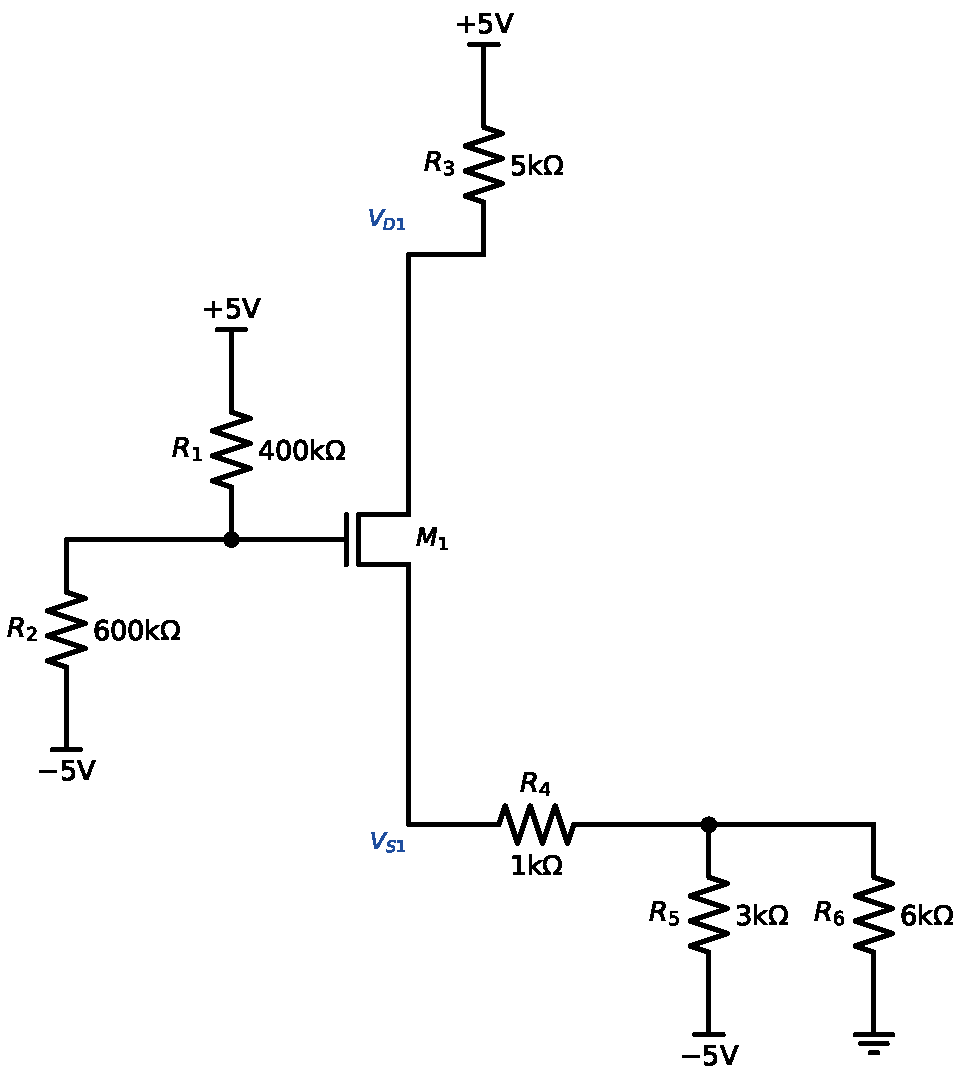
\includegraphics[width=\linewidth,height=7cm,keepaspectratio]{p01_circuit}\end{center}
\end{probbox}

\begin{probbox}{Problem 5F.2 \hfill Easy}
For the circuit below, find the DC drain current of every transistor, the voltages $V_{S1}$, $V_{D1}$ and the operating mode. Assume $k'_p\frac{W}{L} = 850\,\mu \mathrm{A/V^2}$, $V_{tp} = -1.3$\,V. Hint: plain node-by-node KCL is long here; look for a faster way.
\begin{center}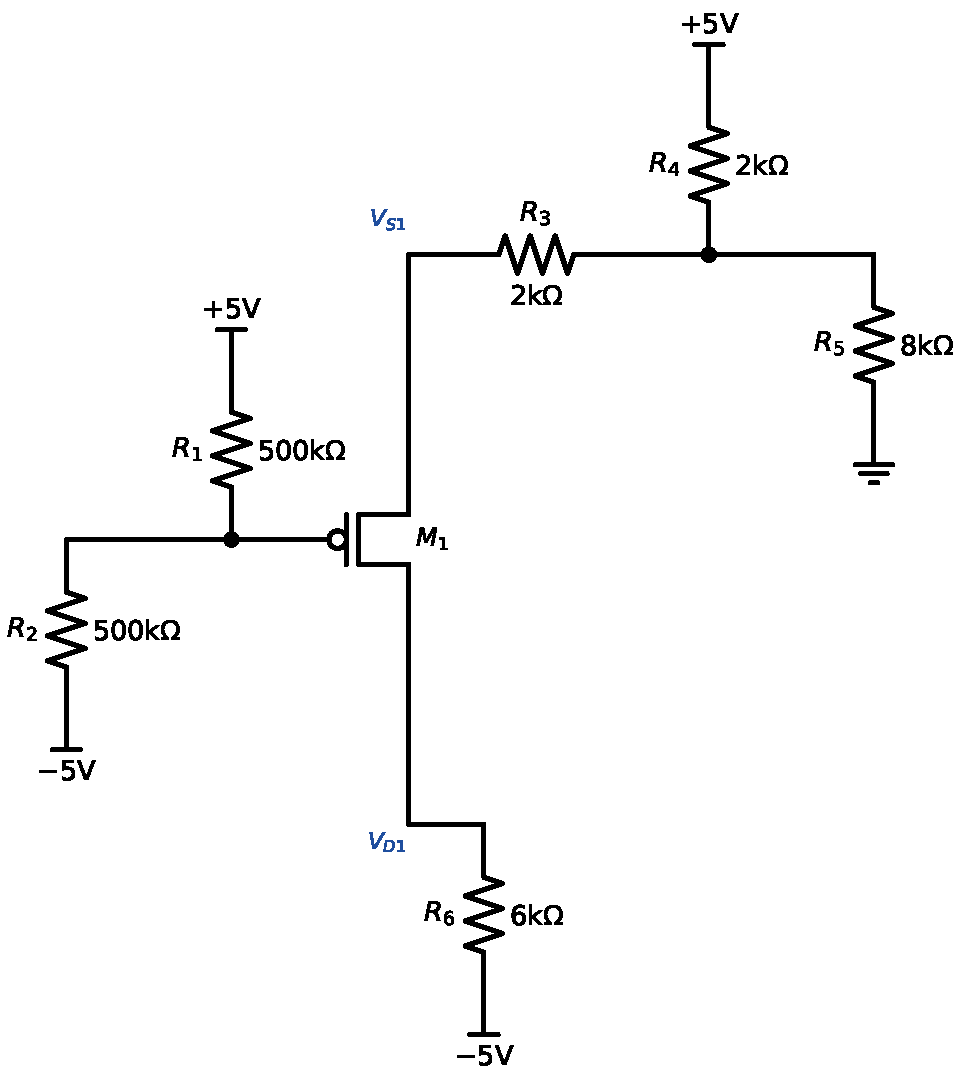
\includegraphics[width=\linewidth,height=7cm,keepaspectratio]{p02_circuit}\end{center}
\end{probbox}

\begin{probbox}{Problem 5F.3 \hfill Easy}
For the circuit below, find the DC drain current of every transistor, the voltages $V_{S1}$, $V_{D1}$ and the operating mode. Assume $k'_n\frac{W}{L} = 1.1\,\mathrm{m}\mathrm{A/V^2}$, $V_{tn} = 1.4$\,V. Hint: plain node-by-node KCL is long here; look for a faster way.
\begin{center}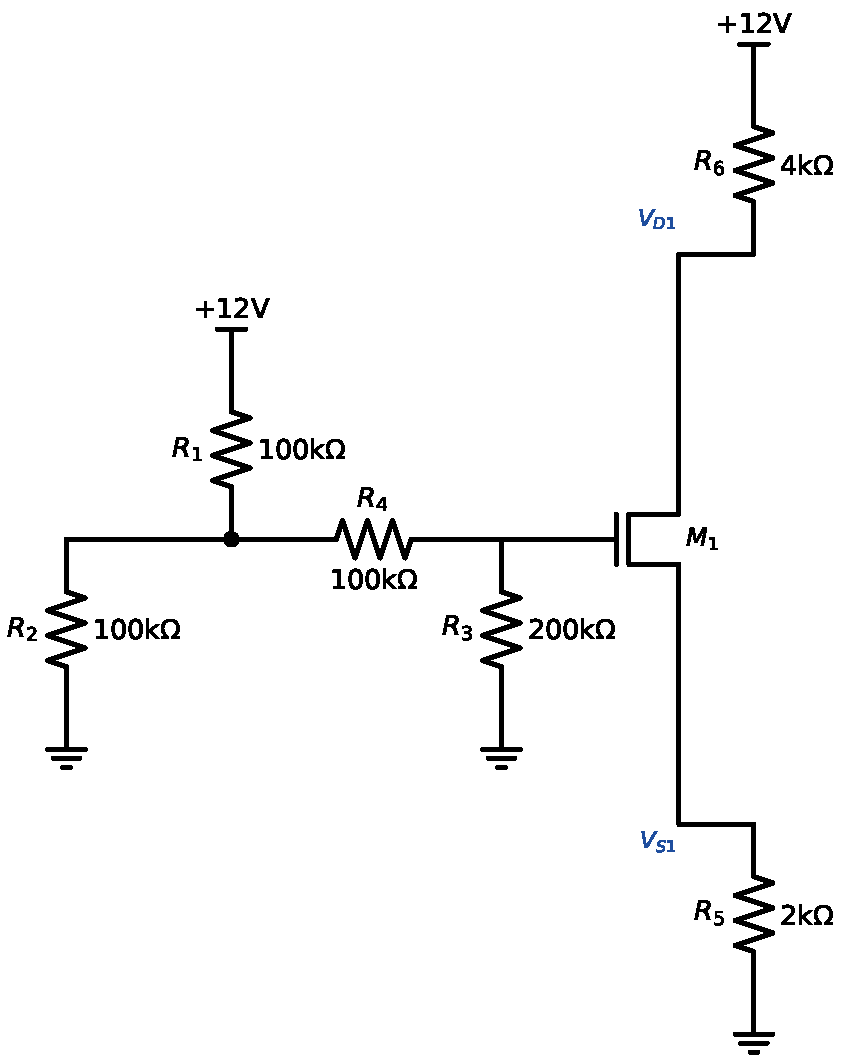
\includegraphics[width=\linewidth,height=7cm,keepaspectratio]{p03_circuit}\end{center}
\end{probbox}

\begin{probbox}{Problem 5F.4 \hfill Easy}
For the circuit below, find the DC drain current of every transistor, the voltages $V_{S1}$, $V_{D1}$ and the operating mode. Assume $k'_n\frac{W}{L} = 1.1\,\mathrm{m}\mathrm{A/V^2}$, $V_{tn} = 1.4$\,V. Hint: plain node-by-node KCL is long here; look for a faster way.
\begin{center}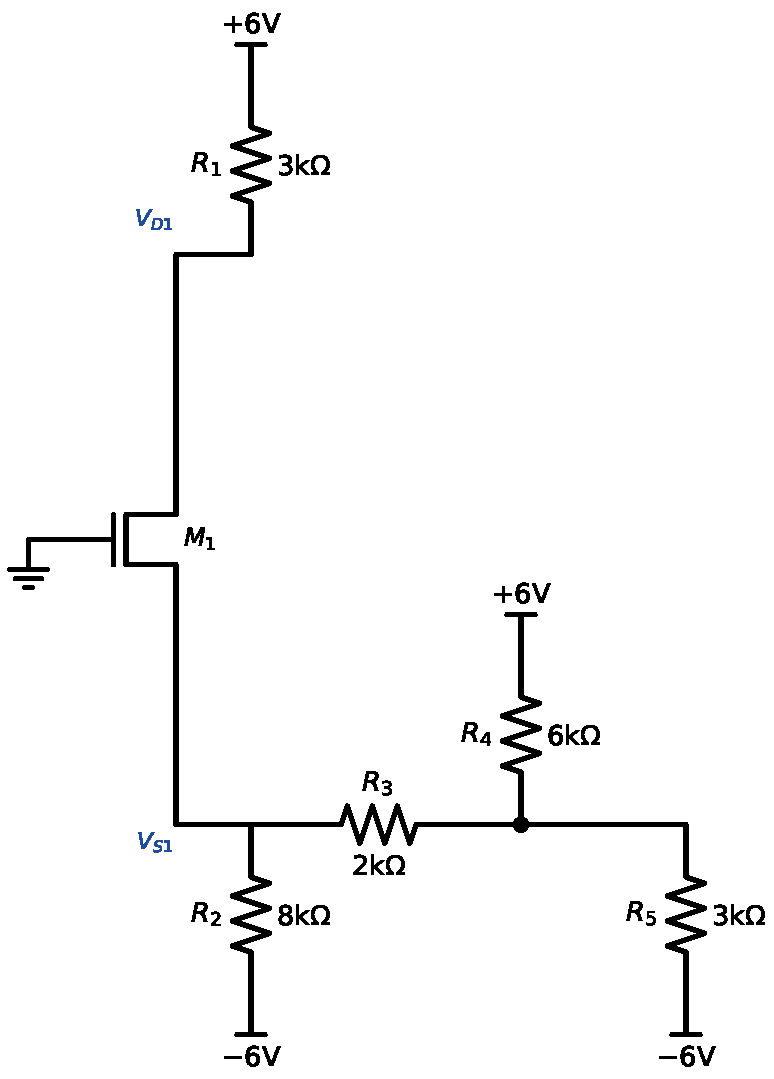
\includegraphics[width=\linewidth,height=7cm,keepaspectratio]{p04_circuit}\end{center}
\end{probbox}

\begin{probbox}{Problem 5F.5 \hfill Easy}
For the amplifier below, find the small-signal transfer function $H(s)=\dfrac{V_o(s)}{V_i(s)}$ and sketch its magnitude Bode plot. Also find the steady-state output $V_o(t)$ for $V_i(t) = 0.01\sin\left(2\pi\cdot 1000\,t\right)$. Assume $k'_n\frac{W}{L} = 1.1\,\mathrm{m}\mathrm{A/V^2}$, $V_{tn} = 1.4$\,V, $r_o = \infty$; the DC drain currents are $I_{D1} = 429\,\mu \mathrm{A}$. Hint: look for a faster way than writing KCL at every node.
\begin{center}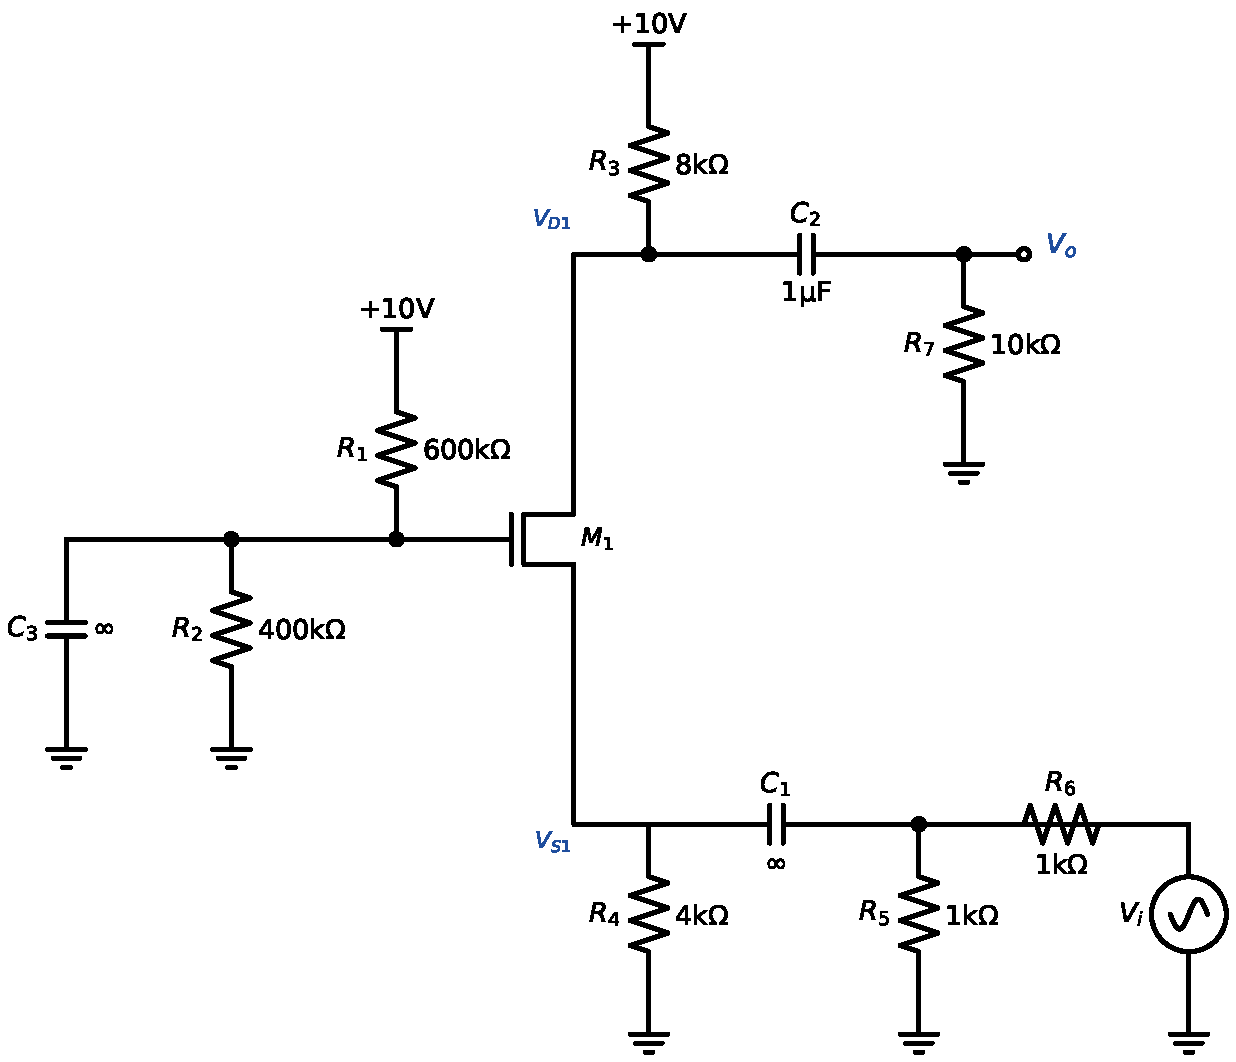
\includegraphics[width=\linewidth,height=7cm,keepaspectratio]{p05_circuit}\end{center}
\end{probbox}

\begin{probbox}{Problem 5F.6 \hfill Easy}
For the amplifier below, find the small-signal transfer function $H(s)=\dfrac{V_o(s)}{V_i(s)}$ and sketch its magnitude Bode plot. Also find the steady-state output $V_o(t)$ for $V_i(t) = 0.02\sin\left(2\pi\cdot 20\,t\right)$. Assume $k'_n\frac{W}{L} = 1.1\,\mathrm{m}\mathrm{A/V^2}$, $V_{tn} = 1.4$\,V, $r_o = \infty$; the DC drain currents are $I_{D1} = 726\,\mu \mathrm{A}$. Hint: look for a faster way than writing KCL at every node.
\begin{center}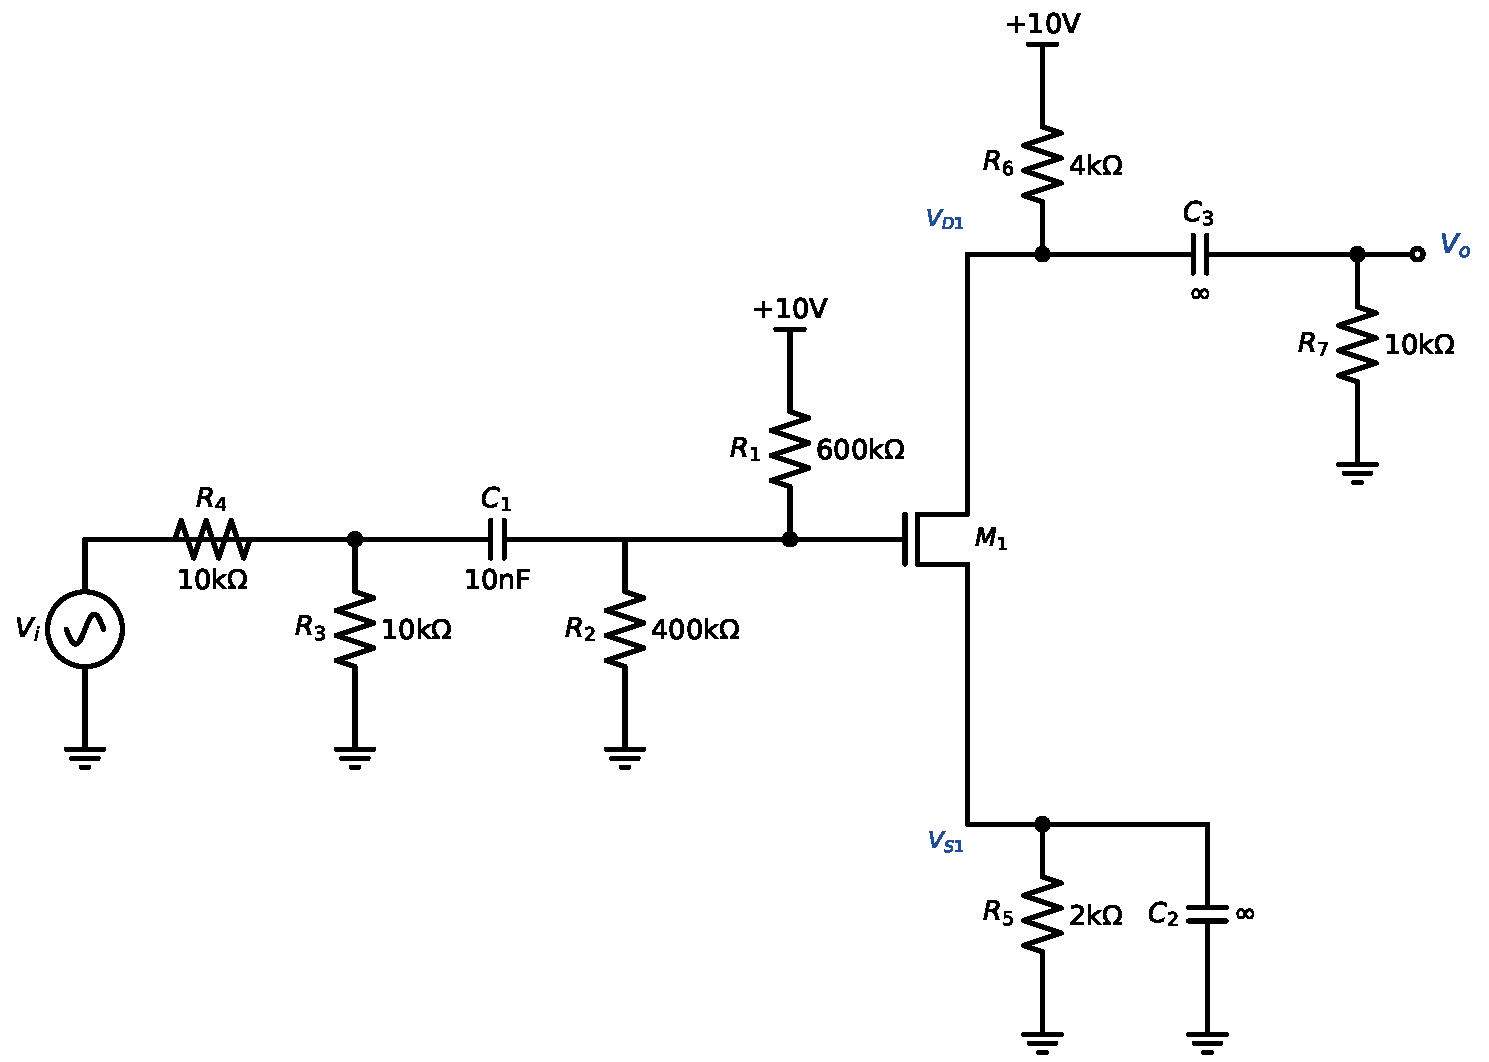
\includegraphics[width=\linewidth,height=7cm,keepaspectratio]{p06_circuit}\end{center}
\end{probbox}

\subsection*{Medium problems}
\begin{probbox}{Problem 5F.7 \hfill Medium}
For the circuit below, find the DC drain current of every transistor, the voltages $V_{S1}$, $V_{D1}$ and the operating mode. Assume $k'_n\frac{W}{L} = 1.1\,\mathrm{m}\mathrm{A/V^2}$, $V_{tn} = 1.4$\,V. Hint: plain node-by-node KCL is long here; look for a faster way.
\begin{center}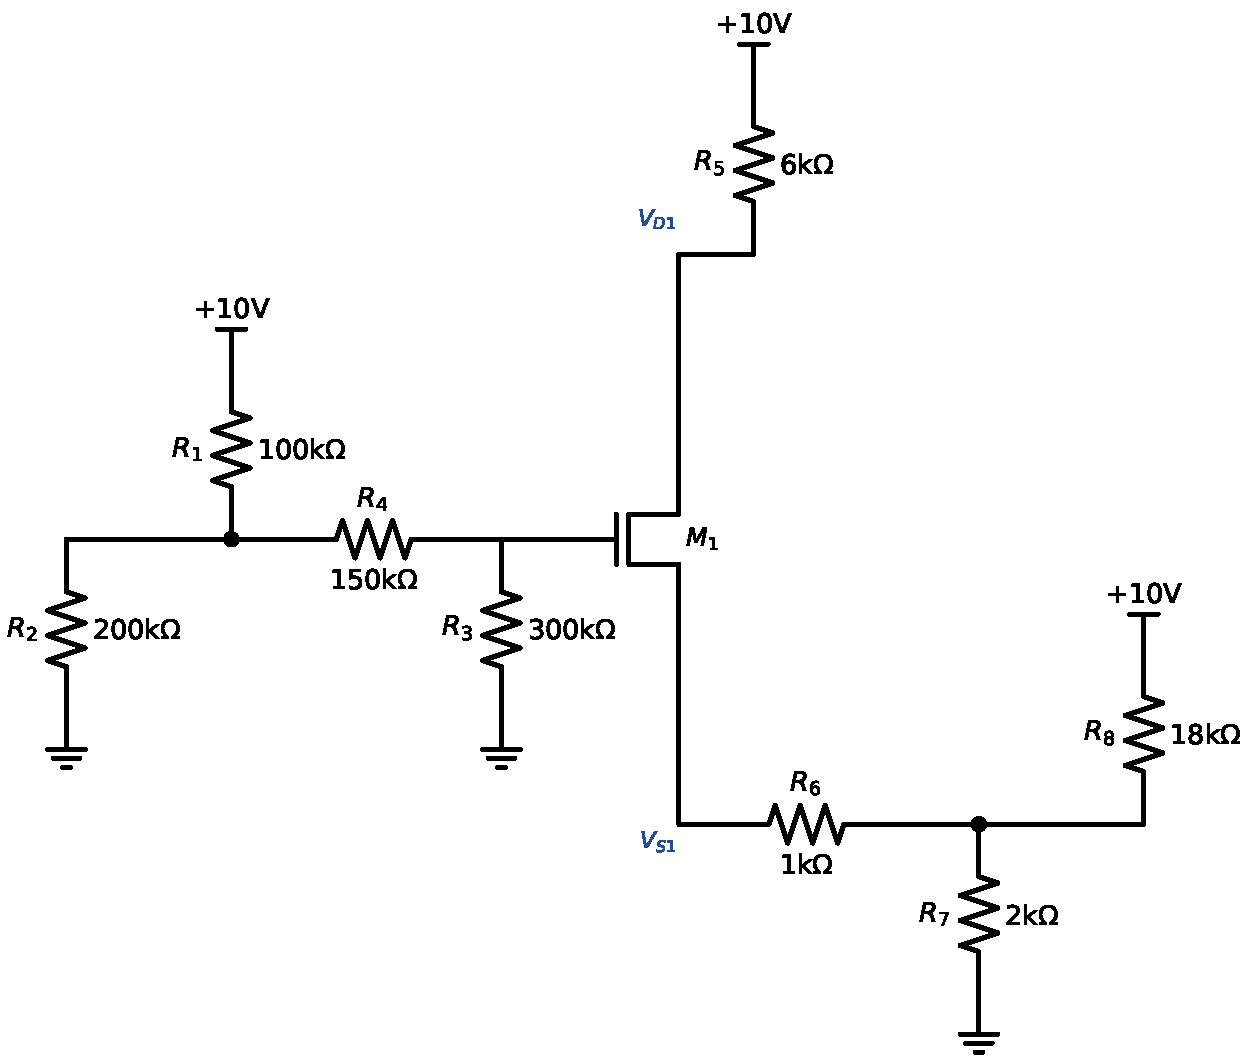
\includegraphics[width=\linewidth,height=7cm,keepaspectratio]{p07_circuit}\end{center}
\end{probbox}

\begin{probbox}{Problem 5F.8 \hfill Medium}
For the circuit below, find the DC drain current of every transistor, the voltages $V_{S1}$, $V_{D1}$ and the operating mode. Assume $k'_p\frac{W}{L} = 850\,\mu \mathrm{A/V^2}$, $V_{tp} = -1.3$\,V. Hint: plain node-by-node KCL is long here; look for a faster way.
\begin{center}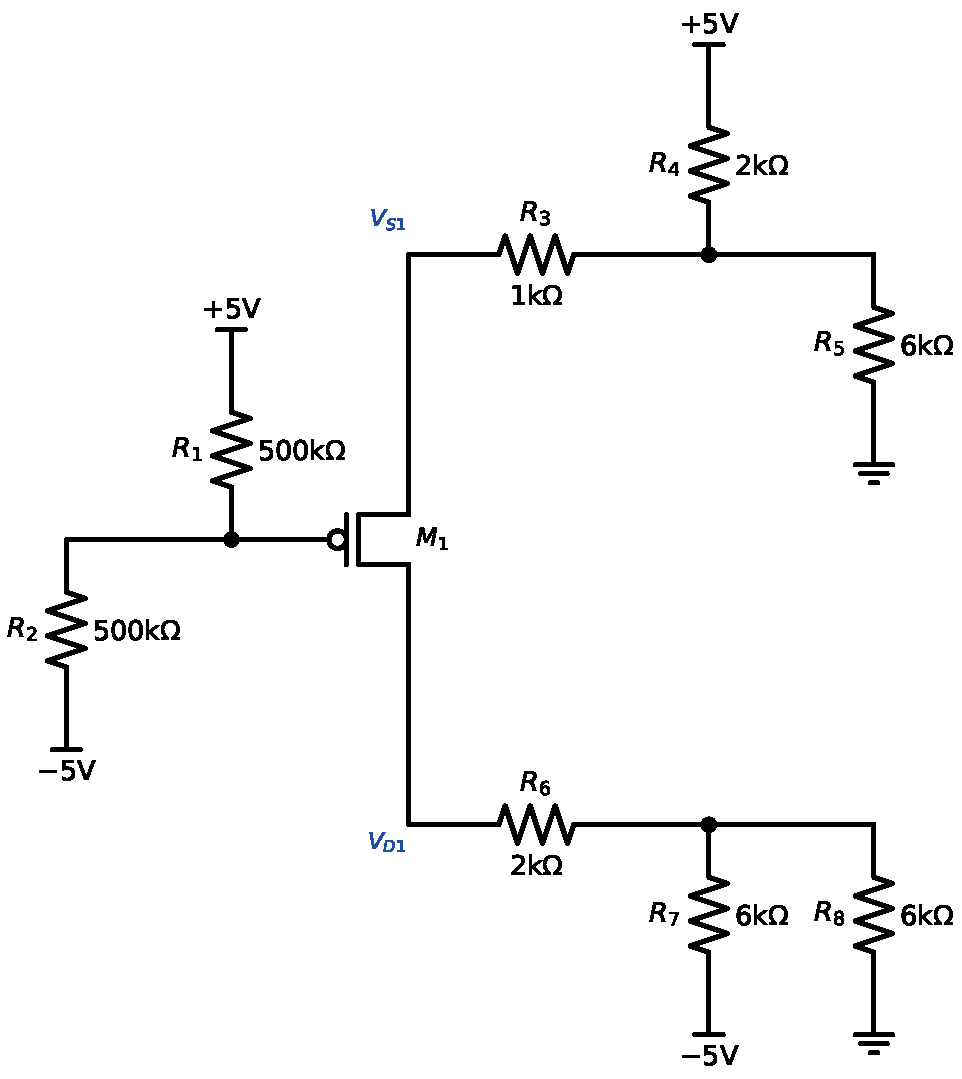
\includegraphics[width=\linewidth,height=7cm,keepaspectratio]{p08_circuit}\end{center}
\end{probbox}

\begin{probbox}{Problem 5F.9 \hfill Medium}
For the circuit below, find the DC drain current of every transistor, the voltages $V_{S1}$, $V_{D1}$ and the operating mode. Assume $k'_n\frac{W}{L} = 1.1\,\mathrm{m}\mathrm{A/V^2}$, $V_{tn} = 1.4$\,V. Hint: plain node-by-node KCL is long here; look for a faster way.
\begin{center}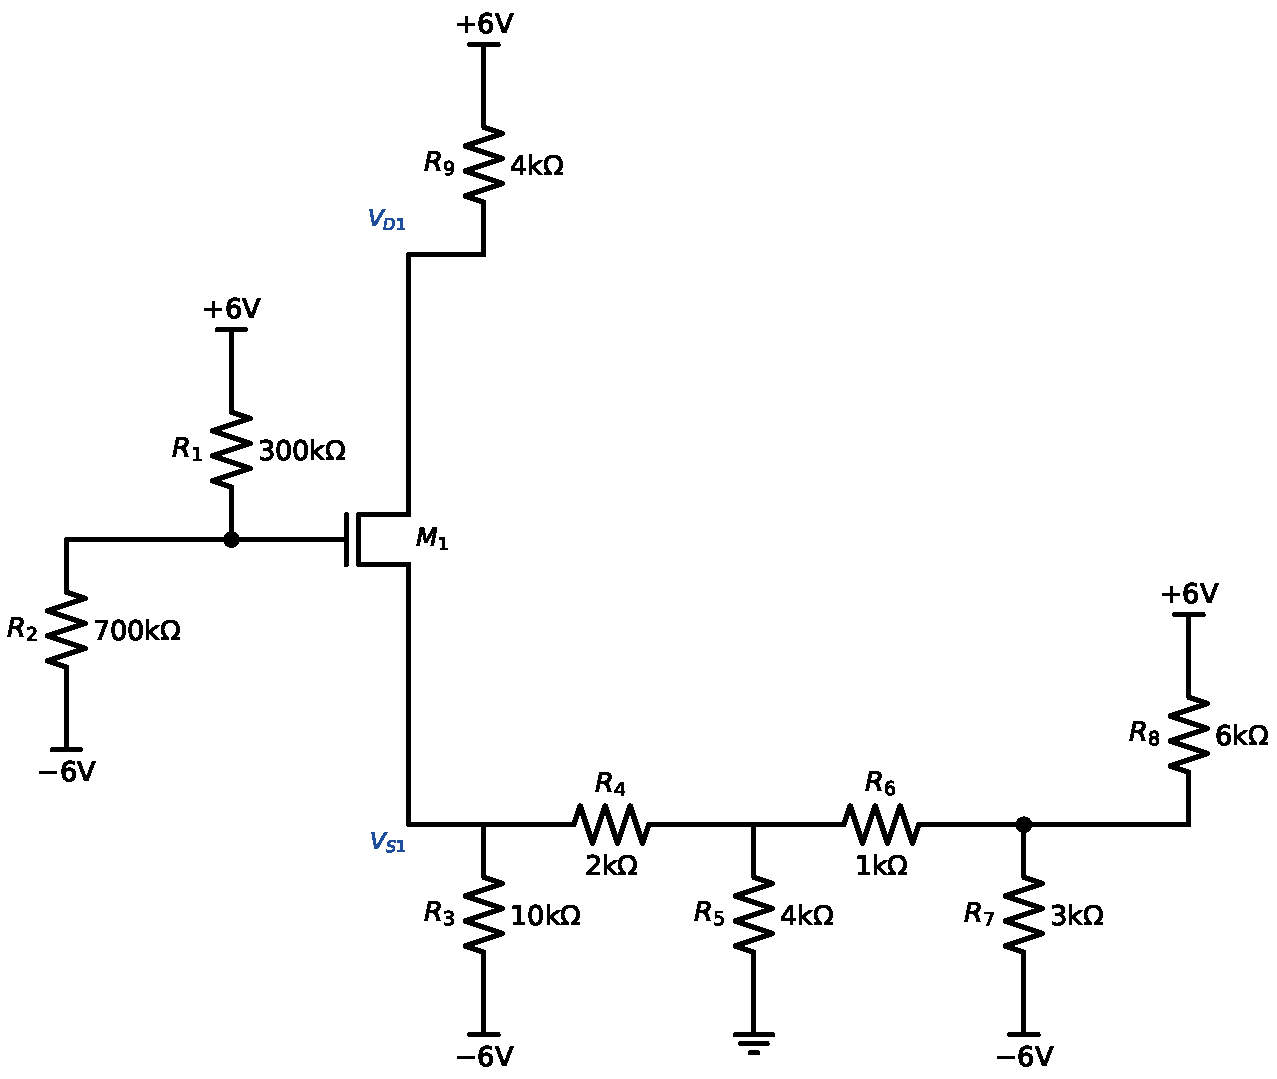
\includegraphics[width=\linewidth,height=7cm,keepaspectratio]{p09_circuit}\end{center}
\end{probbox}

\begin{probbox}{Problem 5F.10 \hfill Medium}
For the amplifier below, find the small-signal transfer function $H(s)=\dfrac{V_o(s)}{V_i(s)}$ and sketch its magnitude Bode plot. Also find the steady-state output $V_o(t)$ for $V_i(t) = 0.01\sin\left(2\pi\cdot 1000\,t\right)$. Assume $k'_n\frac{W}{L} = 1.1\,\mathrm{m}\mathrm{A/V^2}$, $V_{tn} = 1.4$\,V, $r_o = \infty$; the DC drain currents are $I_{D1} = 359\,\mu \mathrm{A}$. Hint: look for a faster way than writing KCL at every node.
\begin{center}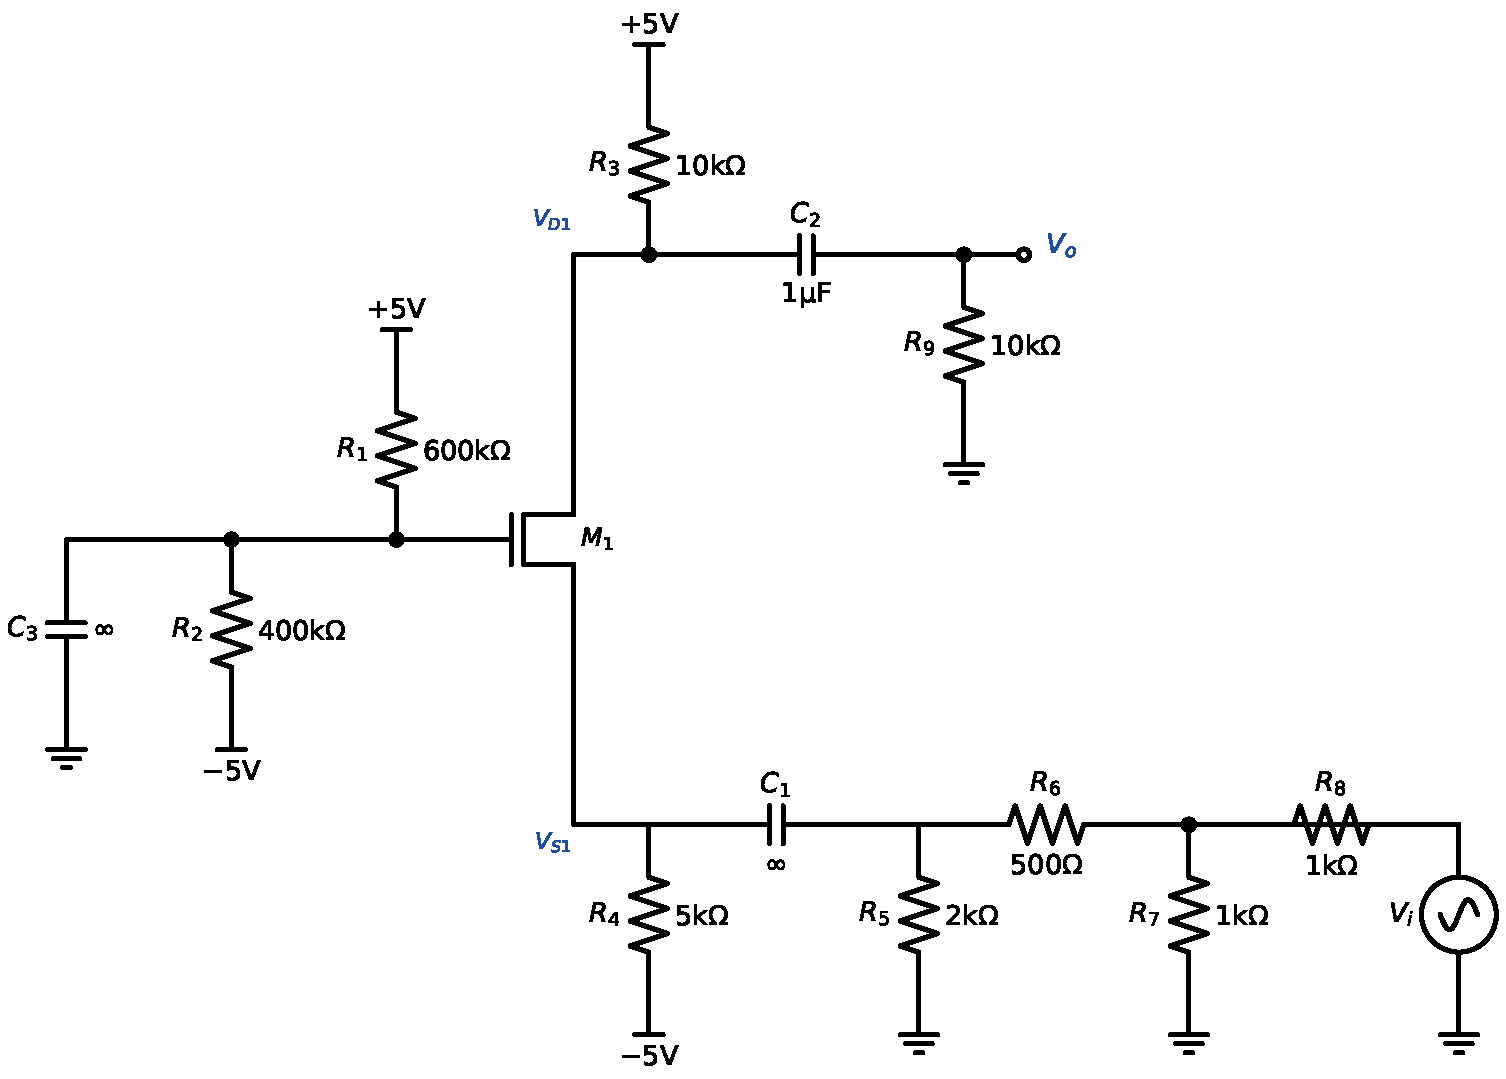
\includegraphics[width=\linewidth,height=7cm,keepaspectratio]{p10_circuit}\end{center}
\end{probbox}

\begin{probbox}{Problem 5F.11 \hfill Medium}
For the amplifier below, find the small-signal transfer function $H(s)=\dfrac{V_o(s)}{V_i(s)}$ and sketch its magnitude Bode plot. Also find the steady-state output $V_o(t)$ for $V_i(t) = 0.01\sin\left(2\pi\cdot 100\,t\right)$. Assume $k'_n\frac{W}{L} = 1.1\,\mathrm{m}\mathrm{A/V^2}$, $V_{tn} = 1.4$\,V, $r_o = \infty$; the DC drain currents are $I_{D1} = 423\,\mu \mathrm{A}$. Hint: look for a faster way than writing KCL at every node.
\begin{center}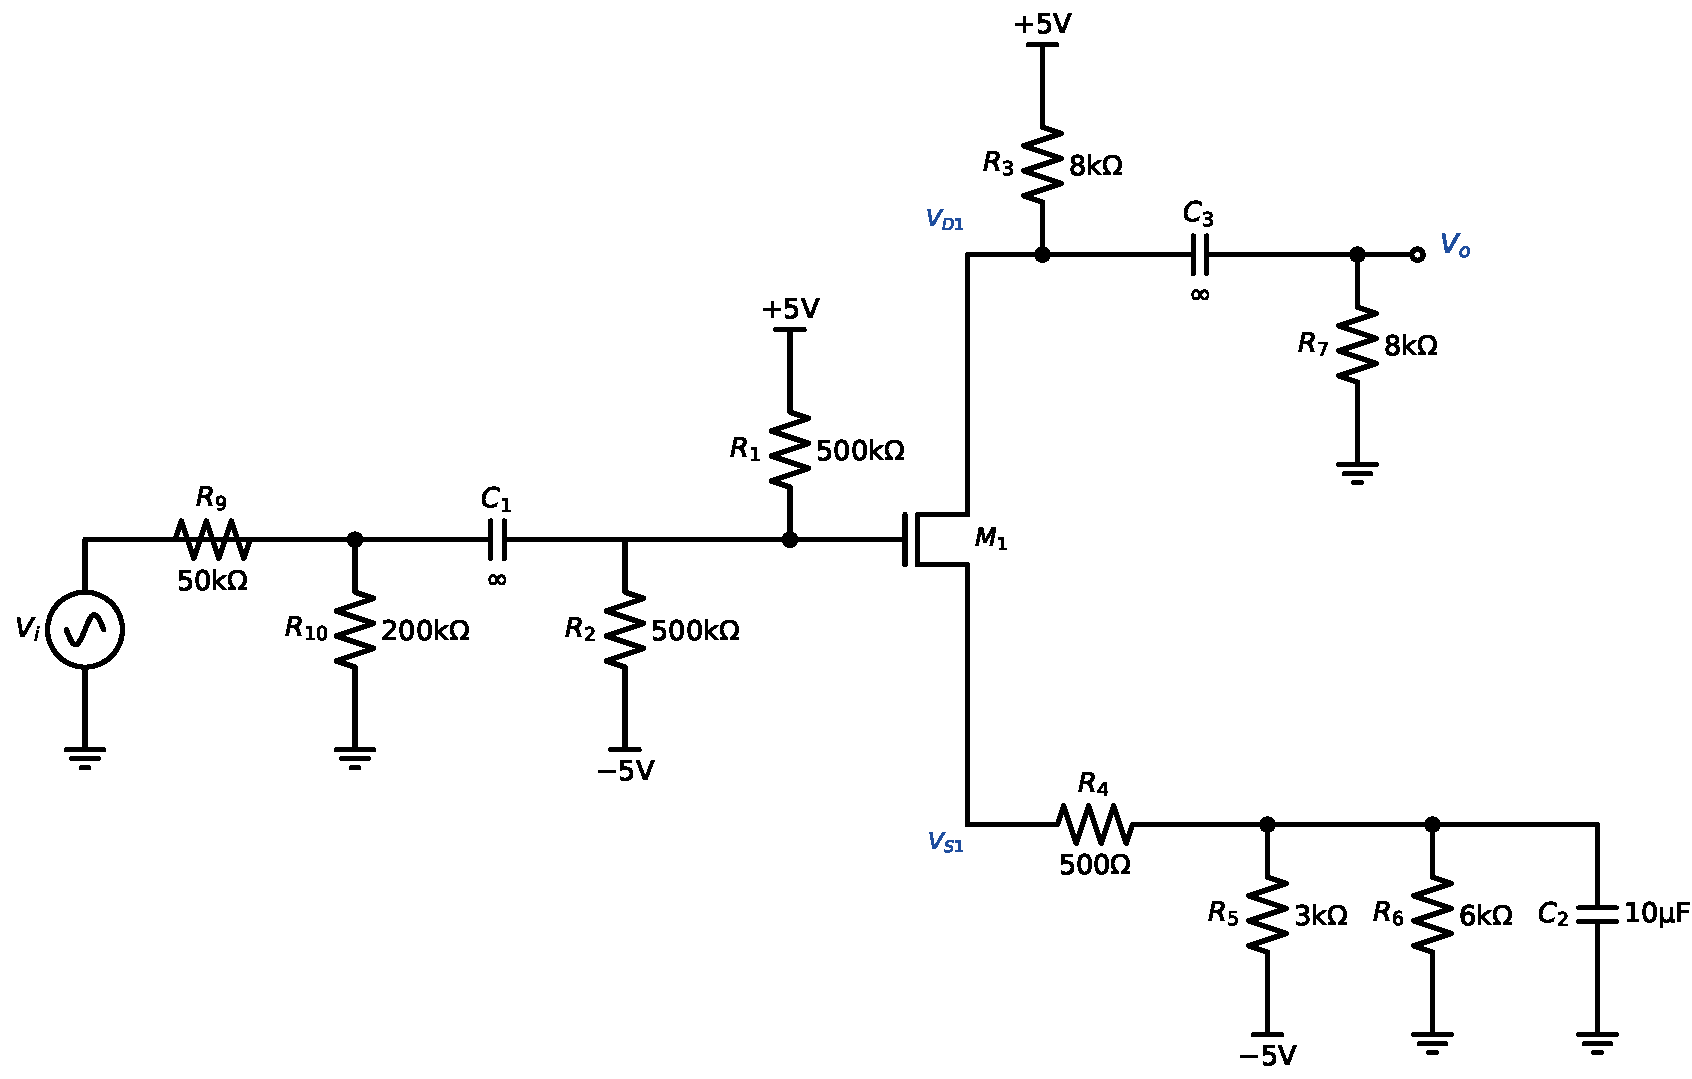
\includegraphics[width=\linewidth,height=7cm,keepaspectratio]{p11_circuit}\end{center}
\end{probbox}

\begin{probbox}{Problem 5F.12 \hfill Medium}
For the amplifier below, find the small-signal transfer function $H(s)=\dfrac{V_o(s)}{V_i(s)}$ and sketch its magnitude Bode plot. Also find the steady-state output $V_o(t)$ for $V_i(t) = 0.5\sin\left(2\pi\cdot 50\,t\right)$. Assume $k'_n\frac{W}{L} = 1.1\,\mathrm{m}\mathrm{A/V^2}$, $V_{tn} = 1.4$\,V, $r_o = \infty$; the DC drain currents are $I_{D1} = 1.37\,\mathrm{m}\mathrm{A}$. Hint: look for a faster way than writing KCL at every node.
\begin{center}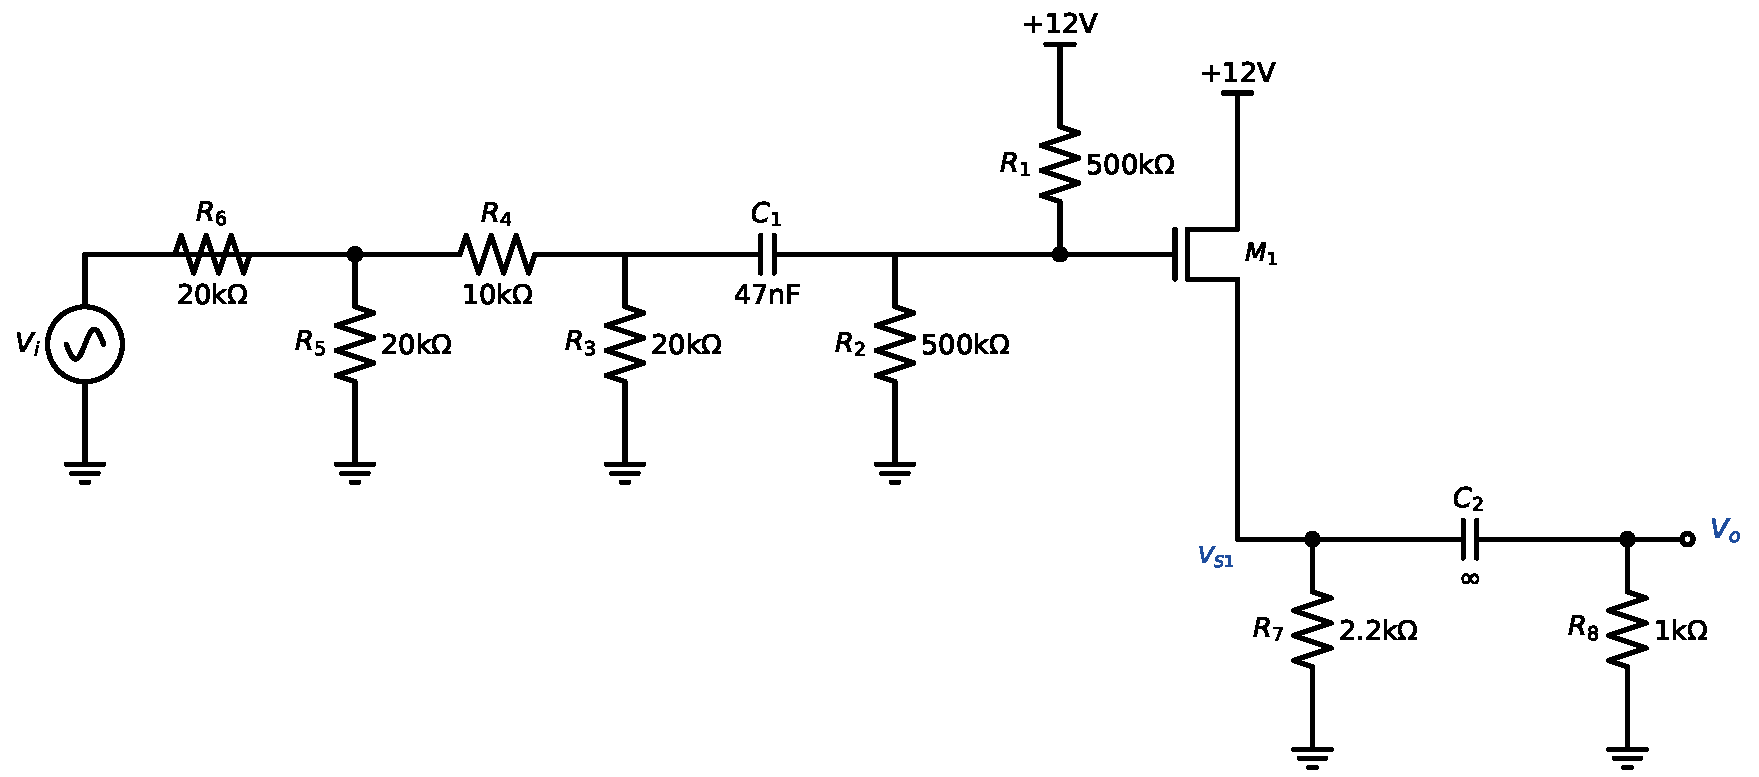
\includegraphics[width=\linewidth,height=7cm,keepaspectratio]{p12_circuit}\end{center}
\end{probbox}

\subsection*{Hard problems}
\begin{probbox}{Problem 5F.13 \hfill Hard}
For the circuit below, find the DC drain current of every transistor, the voltages $V_{S1}$, $V_{D1}$, $V_{S2}$, $V_{D2}$ and the operating mode. Assume $k'_n\frac{W}{L} = 1.1\,\mathrm{m}\mathrm{A/V^2}$, $V_{tn} = 1.4$\,V, $k'_p\frac{W}{L} = 850\,\mu \mathrm{A/V^2}$, $V_{tp} = -1.3$\,V. Hint: plain node-by-node KCL is long here; look for a faster way.
\begin{center}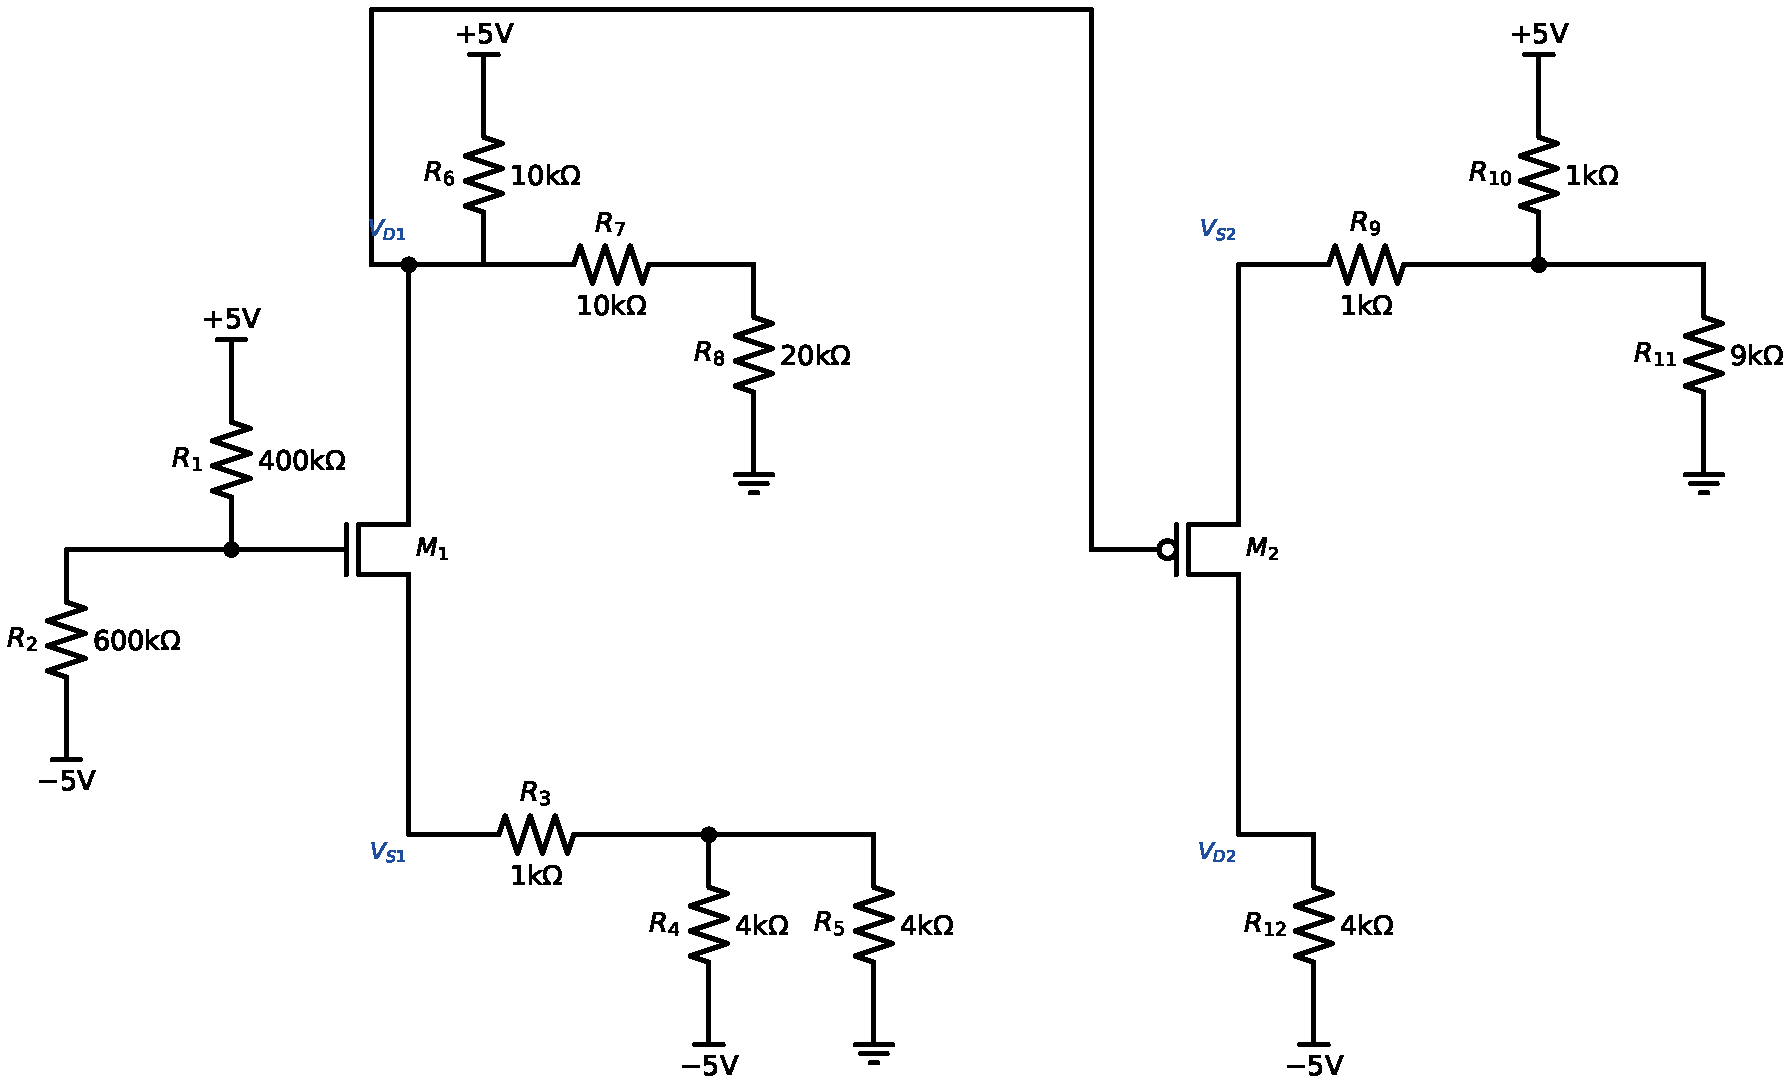
\includegraphics[width=\linewidth,height=7cm,keepaspectratio]{p13_circuit}\end{center}
\end{probbox}

\begin{probbox}{Problem 5F.14 \hfill Hard}
For the circuit below, find the DC drain current of every transistor, the voltages $V_{S1}$, $V_{D1}$ and the operating mode. Assume $k'_n\frac{W}{L} = 1.1\,\mathrm{m}\mathrm{A/V^2}$, $V_{tn} = 1.4$\,V. Hint: plain node-by-node KCL is long here; look for a faster way.
\begin{center}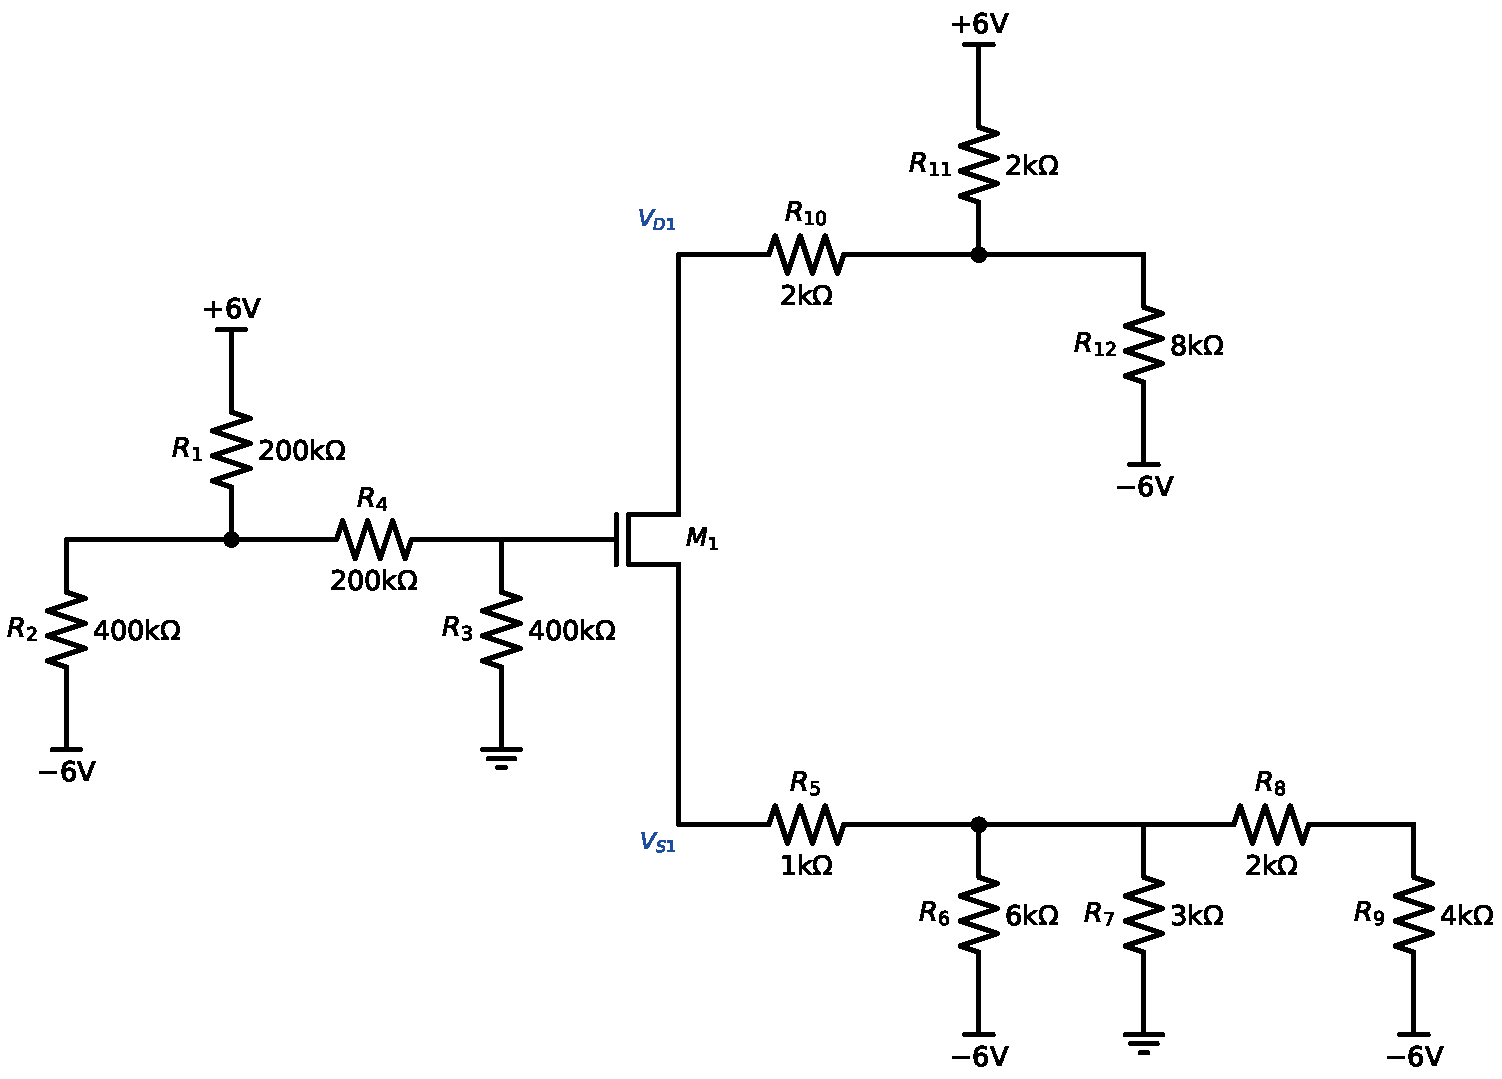
\includegraphics[width=\linewidth,height=7cm,keepaspectratio]{p14_circuit}\end{center}
\end{probbox}

\begin{probbox}{Problem 5F.15 \hfill Hard}
For the circuit below, find the DC drain current of every transistor, the voltages $V_{S1}$, $V_{D1}$, $V_{S2}$, $V_{D2}$ and the operating mode. Assume $k'_n\frac{W}{L} = 1.1\,\mathrm{m}\mathrm{A/V^2}$, $V_{tn} = 1.4$\,V, $k'_p\frac{W}{L} = 850\,\mu \mathrm{A/V^2}$, $V_{tp} = -1.3$\,V. Hint: plain node-by-node KCL is long here; look for a faster way.
\begin{center}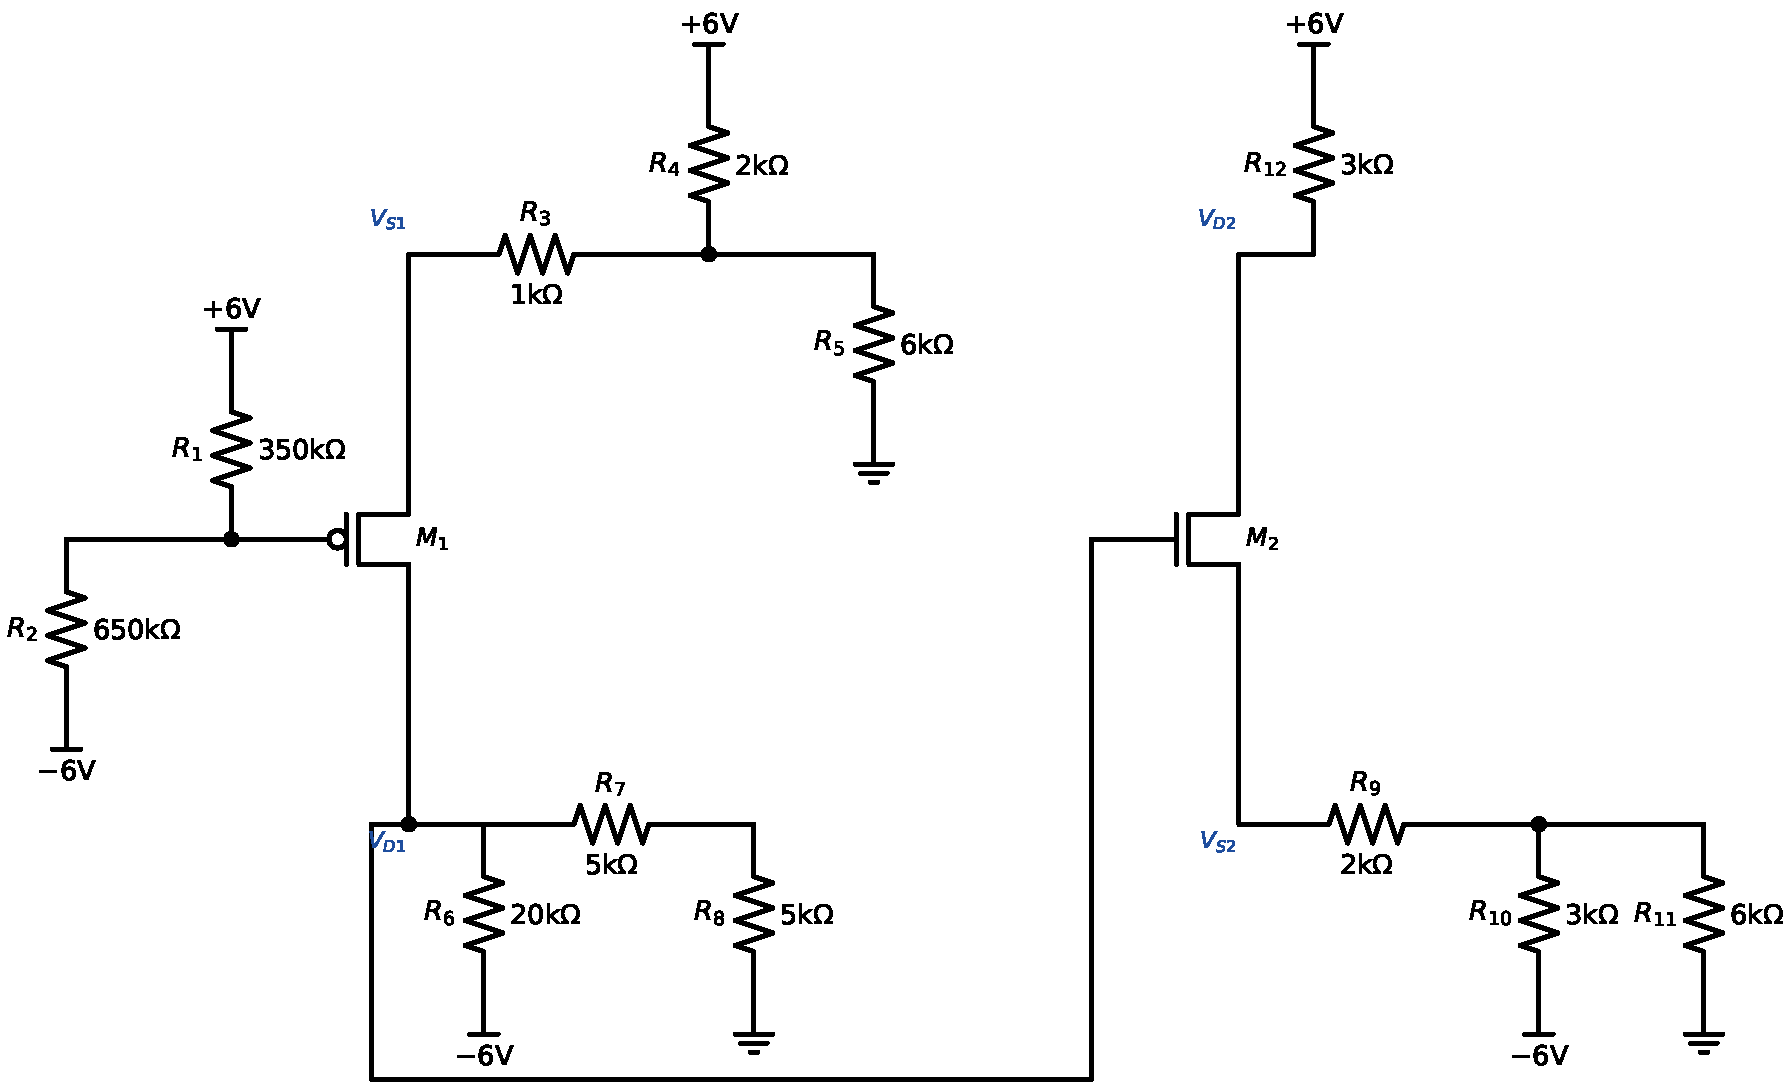
\includegraphics[width=\linewidth,height=7cm,keepaspectratio]{p15_circuit}\end{center}
\end{probbox}

\begin{probbox}{Problem 5F.16 \hfill Hard}
For the amplifier below, find the small-signal transfer function $H(s)=\dfrac{V_o(s)}{V_i(s)}$ and sketch its magnitude Bode plot. Also find the steady-state output $V_o(t)$ for $V_i(t) = 0.01\sin\left(2\pi\cdot 1000\,t\right)$. Assume $k'_n\frac{W}{L} = 1.1\,\mathrm{m}\mathrm{A/V^2}$, $V_{tn} = 1.4$\,V, $r_o = \infty$; the DC drain currents are $I_{D1} = 726\,\mu \mathrm{A}$. Hint: look for a faster way than writing KCL at every node.
\begin{center}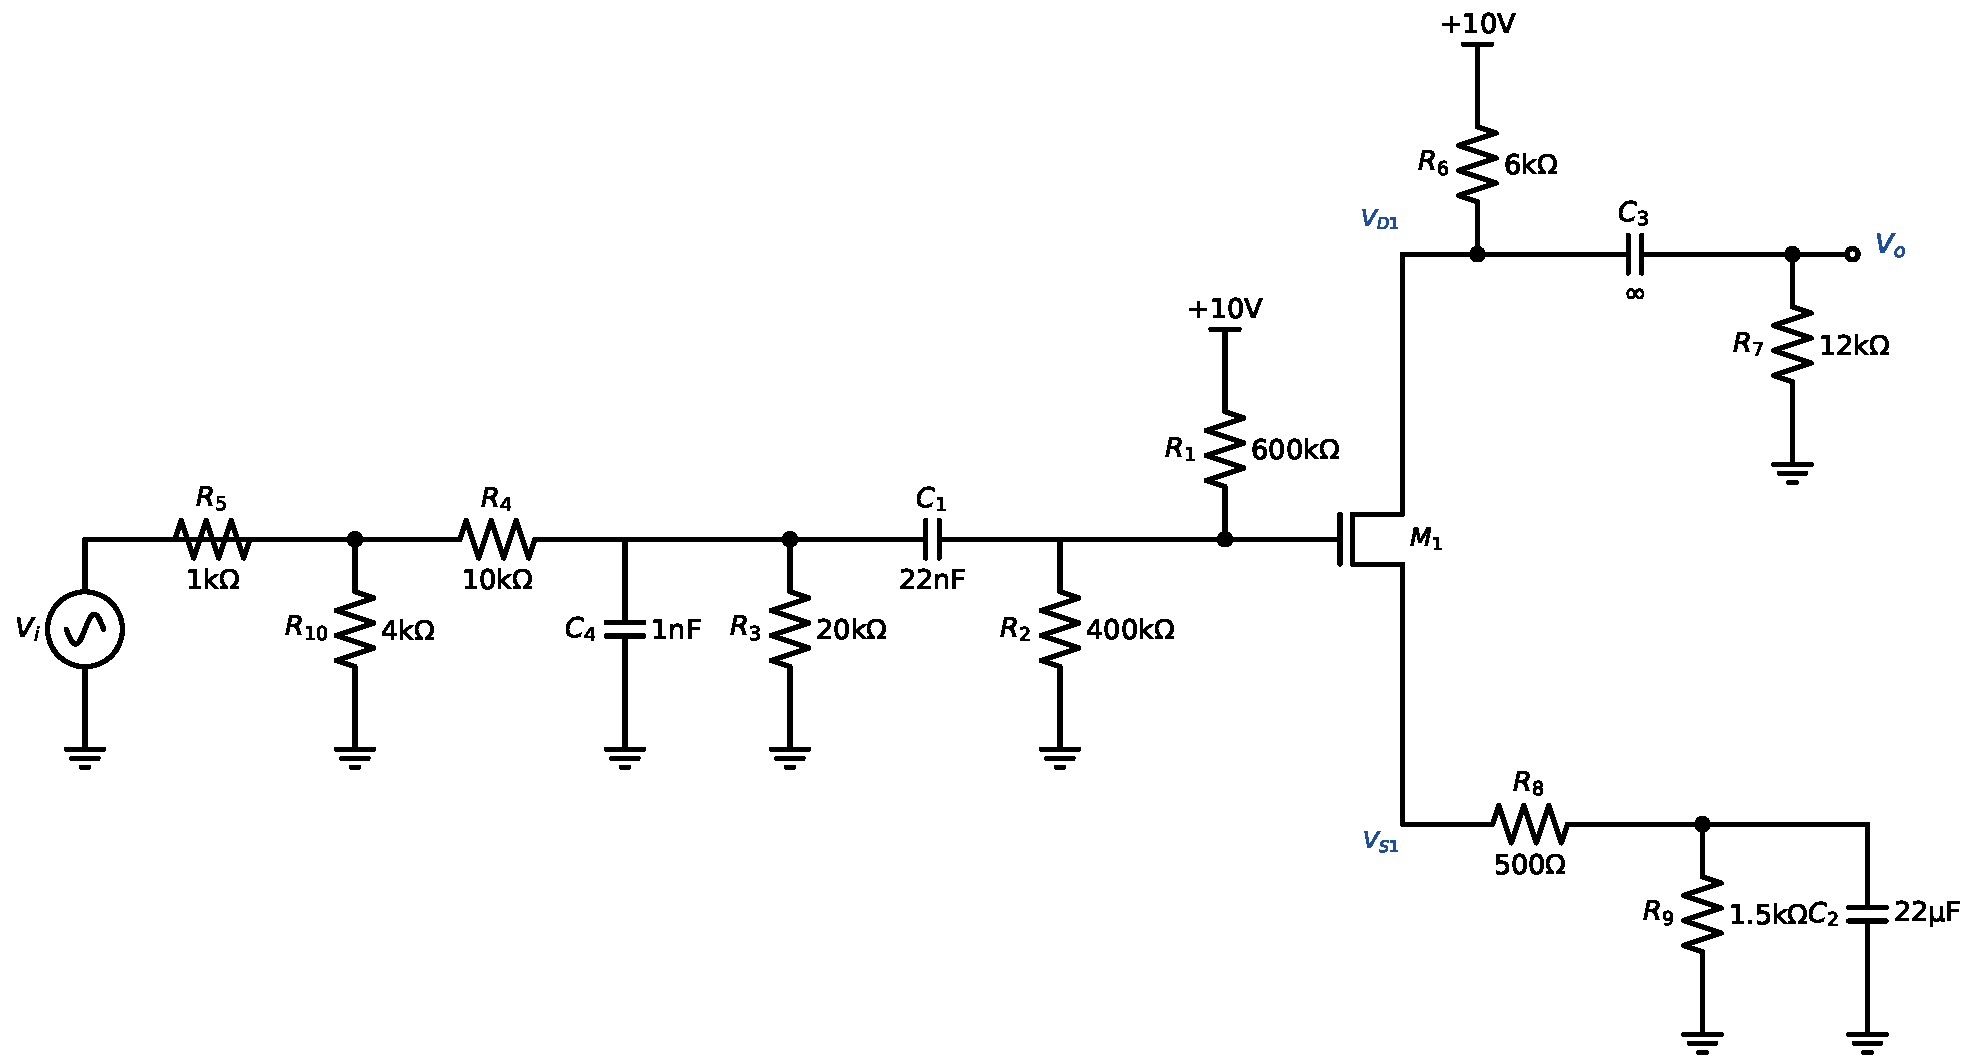
\includegraphics[width=\linewidth,height=7cm,keepaspectratio]{p16_circuit}\end{center}
\end{probbox}

\begin{probbox}{Problem 5F.17 \hfill Hard}
For the amplifier below, find the small-signal transfer function $H(s)=\dfrac{V_o(s)}{V_i(s)}$ and sketch its magnitude Bode plot. Also find the steady-state output $V_o(t)$ for $V_i(t) = 0.01\sin\left(2\pi\cdot 500\,t\right)$. Assume $k'_n\frac{W}{L} = 1.1\,\mathrm{m}\mathrm{A/V^2}$, $V_{tn} = 1.4$\,V, $r_o = \infty$; the DC drain currents are $I_{D1} = 429\,\mu \mathrm{A}$. Hint: look for a faster way than writing KCL at every node.
\begin{center}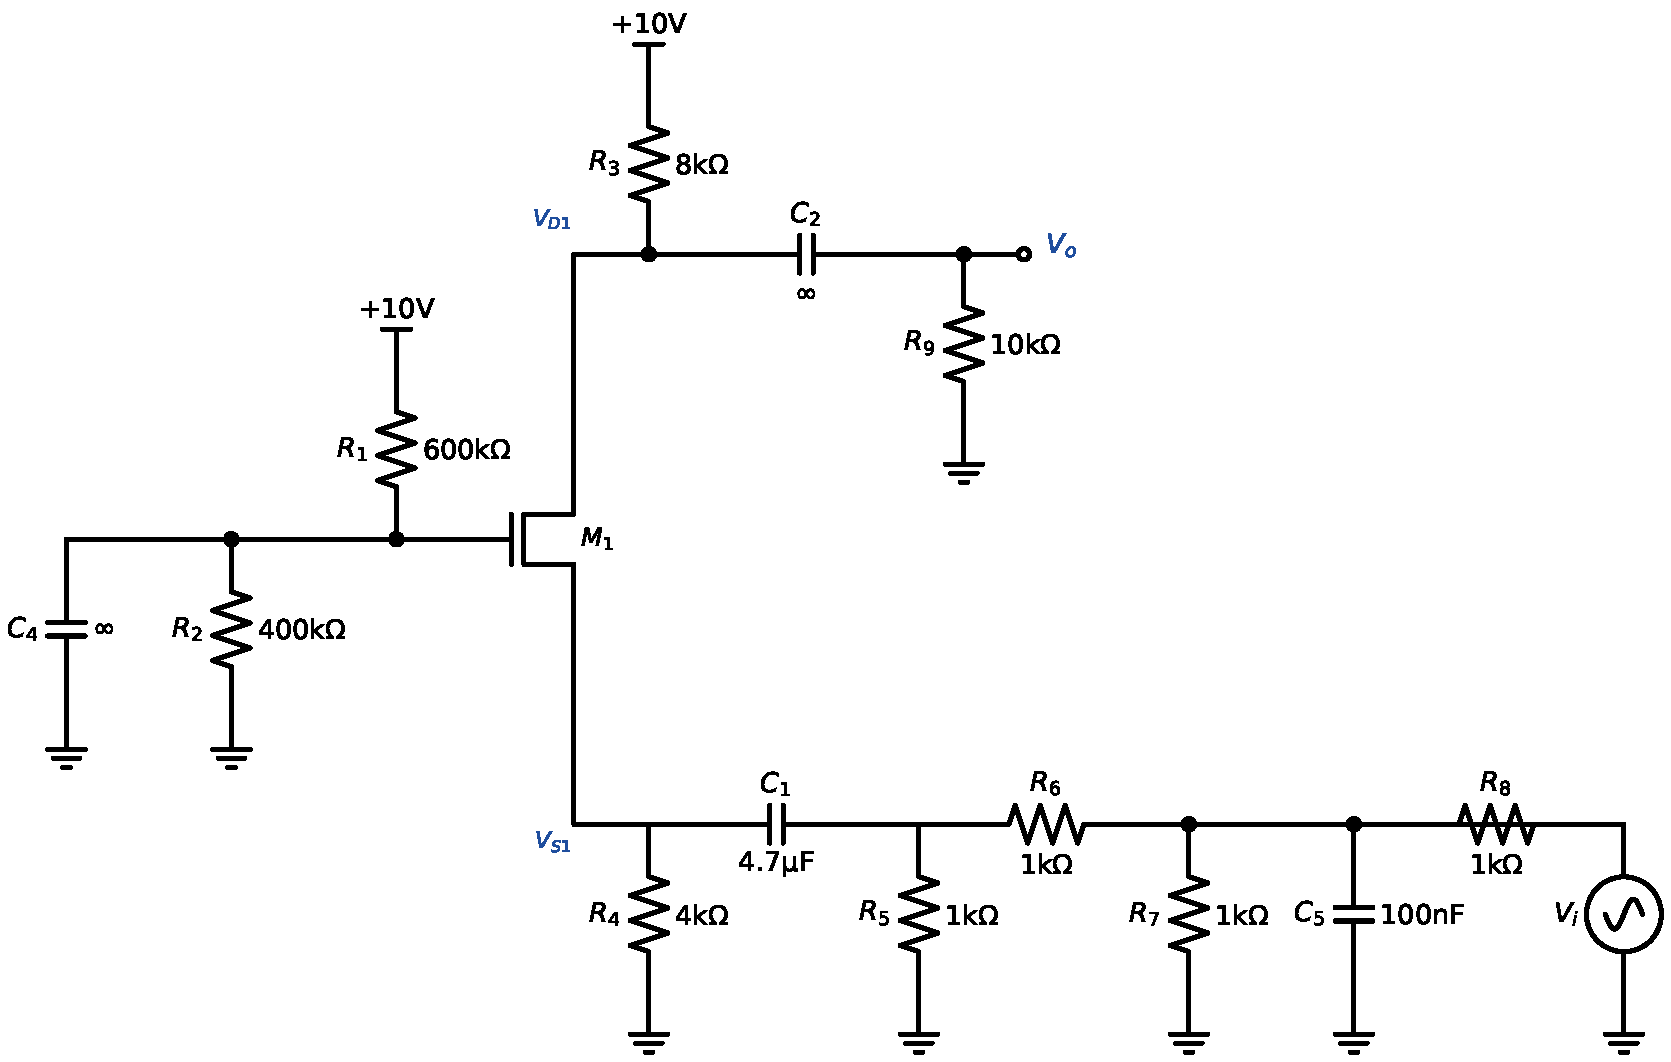
\includegraphics[width=\linewidth,height=7cm,keepaspectratio]{p17_circuit}\end{center}
\end{probbox}

\begin{probbox}{Problem 5F.18 \hfill Hard}
For the amplifier below, find the small-signal transfer function $H(s)=\dfrac{V_o(s)}{V_i(s)}$ and sketch its magnitude Bode plot. Also find the steady-state output $V_o(t)$ for $V_i(t) = 0.01\sin\left(2\pi\cdot 100\,t\right)$. Assume $k'_n\frac{W}{L} = 1.1\,\mathrm{m}\mathrm{A/V^2}$, $V_{tn} = 1.4$\,V, $r_o = \infty$; the DC drain currents are $I_{D1} = 726\,\mu \mathrm{A}$, $I_{D2} = 1.17\,\mathrm{m}\mathrm{A}$. Hint: look for a faster way than writing KCL at every node.
\begin{center}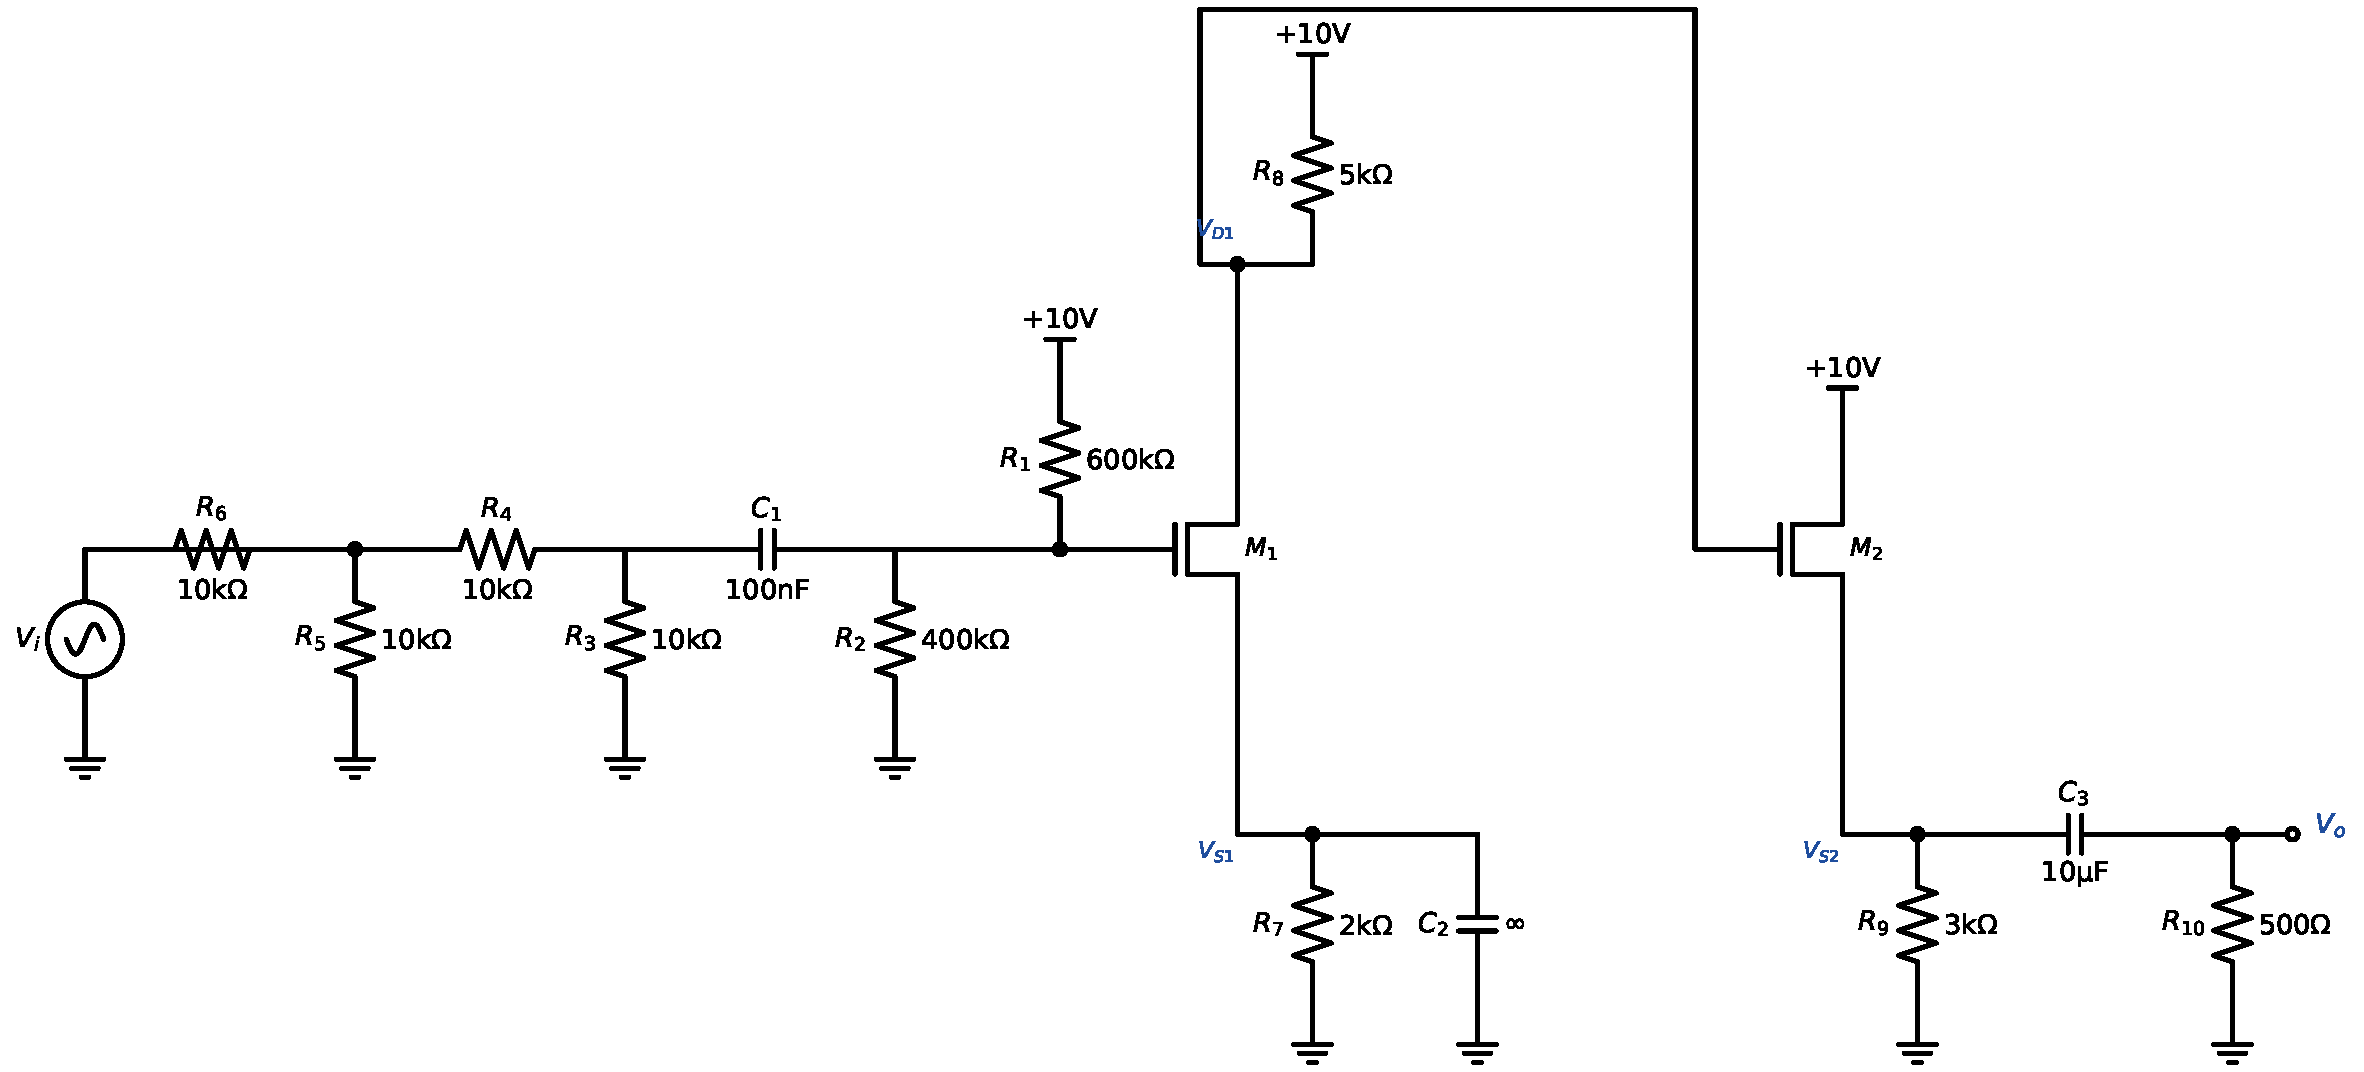
\includegraphics[width=\linewidth,height=7cm,keepaspectratio]{p18_circuit}\end{center}
\end{probbox}

\newpage
\section*{Solutions}
Every solution follows the steps of the Lecture-5 pipeline card.
\subsection*{Solution 5F.1 \hfill Easy}
\begin{center}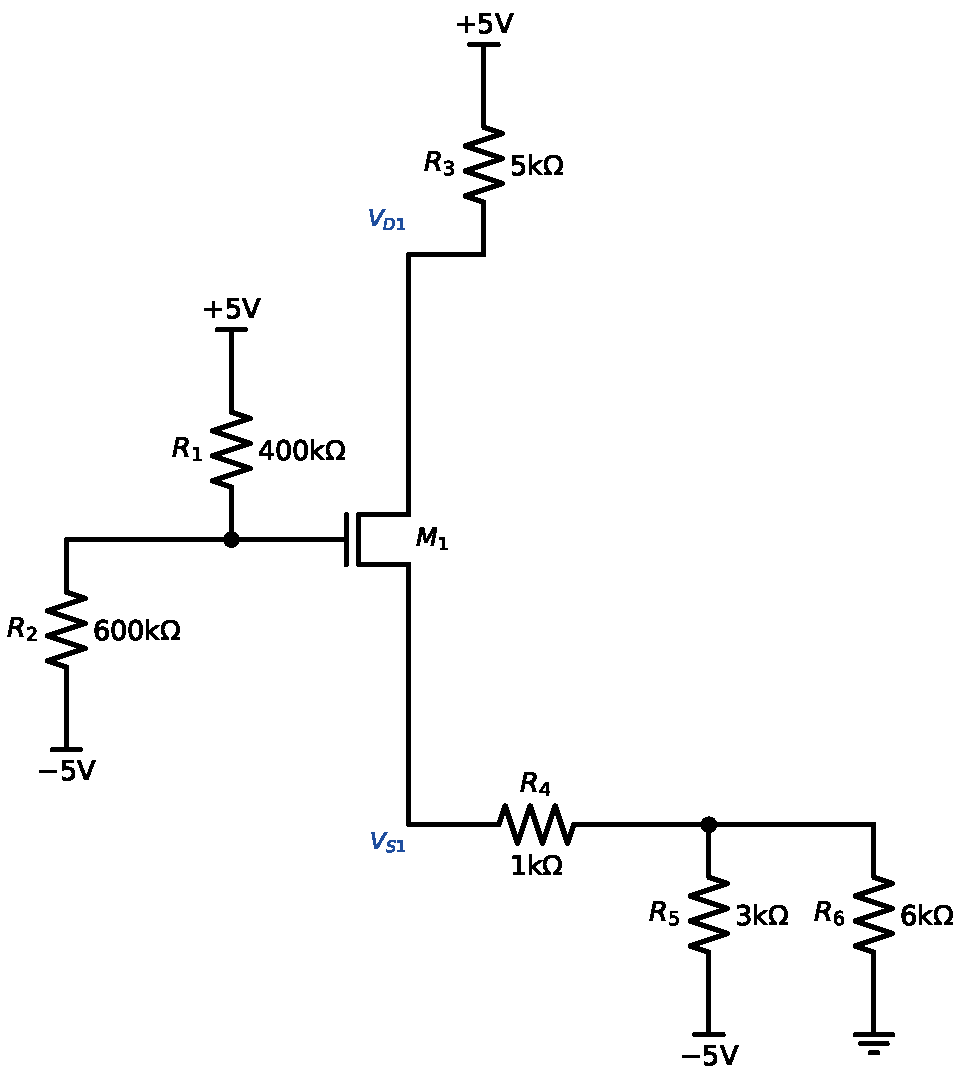
\includegraphics[width=0.9\linewidth,height=6cm,keepaspectratio]{p01_circuit}\end{center}
\solstep{1}{Why Thevenin}Plain KCL would need all 4 unknown node voltages at once, and the transistor equation is quadratic, so the elimination by hand is long. But each transistor touches every resistor network at a single terminal, and the gate draws no current. So every network can be replaced by its Thevenin pair $(V_{th}, R_{th})$ (tool T5), computed with the transistor removed --- 3 small networks, each a chain of dividers. What is left is one loop per transistor with a single quadratic.
\solstep{2}{Transistor $M_{1}$}\emph{Gate network} (seen from the gate of $M_{1}$, transistor removed). At $V_{G1}$ combine in parallel $R_{1}$ to $5$, $R_{2}$ to $(-5)$ (Millman): \[V_{th} = \frac{\sum V_k/R_k}{\sum 1/R_k} = 1\,\mathrm{V},\qquad R_{th} = 400\,\mathrm{k}\Omega \| 600\,\mathrm{k}\Omega = 240\,\mathrm{k}\Omega\] No current flows into the gate, so only $V_{th}$ matters: $V_{G1} = V_{th,G1} = 1\,\mathrm{V}$.

\emph{Source network} (seen from the source of $M_{1}$). At $V_{x1}$ combine in parallel $R_{5}$ to $(-5)$, $R_{6}$ to $0$ (Millman): \[V_{th} = \frac{\sum V_k/R_k}{\sum 1/R_k} = -3.333\,\mathrm{V},\qquad R_{th} = 3\,\mathrm{k}\Omega \| 6\,\mathrm{k}\Omega = 2\,\mathrm{k}\Omega\] Through $R_{4}$ in series: $R_{th}$ grows by $R_{4}$: $(V_{th}, R_{th}) = (-3.333\,\mathrm{V},\ 3\,\mathrm{k}\Omega)$.

\emph{Drain network} (seen from the drain of $M_{1}$). Start at $V_{D1}$: only $R_{3}$ to $5$, i.e. $(V_{th}, R_{th}) = (5\,\mathrm{V},\ 5\,\mathrm{k}\Omega)$.

With the networks replaced, $M_{1}$ sees one loop: gate at $1\,\mathrm{V}$, source through $R_{th,S1} = 3\,\mathrm{k}\Omega$ to $V_{th,S1} = -3.33\,\mathrm{V}$. KVL (assume $M_{1}$ active):\[V_{G1} - V_{th,S1} = 4.333 = V_{GS1} + R_{th,S1}I_{D1},\qquad I_{D1} = \frac{1.1\,\mathrm{m}}{2}(V_{GS1} - 1.4)^2\]\[1.65V_{GS1}^2 - 3.62V_{GS1} - 1.099 = 0 \;\Rightarrow\; V_{GS1} = -0.2704\ \text{or}\ 2.464\,\mathrm{V}\]The root $-0.27$\,V is below $|V_t| = 1.4$\,V (the transistor would be off), so $V_{GS1} = 2.464$\,V. So $I_{D1} = 623\,\mu \mathrm{A}$.

Terminal voltages: $V_{S1} = V_{G1} - V_{GS1} = -1.46\,\mathrm{V}$, $V_{D1} = V_{th,D1} - R_{th,D1}I_{D1} = 5 - 5\,\mathrm{k}\times623\,\mu \mathrm{A} = 1.88\,\mathrm{V}$.

Check: $V_{DS1} = 3.349$\,V $\ge V_{ov1} = 1.06$\,V: $M_{1}$ is active \checkmark
\solstep{3}{Equivalent circuit}With every network replaced by its Thevenin pair the circuit is just this (the solution above is the analysis of this circuit):\begin{center}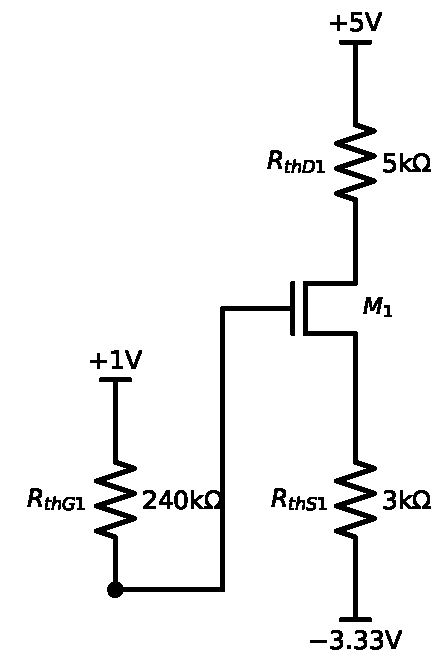
\includegraphics[width=0.6\linewidth,height=5cm,keepaspectratio]{p01_equivalent}\end{center}

A full nodal solve of the original circuit (all 4 node voltages) gives the same currents.
\begin{ansbox}
$I_{D1} = 623\,\mu \mathrm{A}$, $V_{S1} = -1.46\,\mathrm{V}$, $V_{D1} = 1.88\,\mathrm{V}$\\[2pt] all transistors active.
\end{ansbox}

\newpage
\subsection*{Solution 5F.2 \hfill Easy}
\begin{center}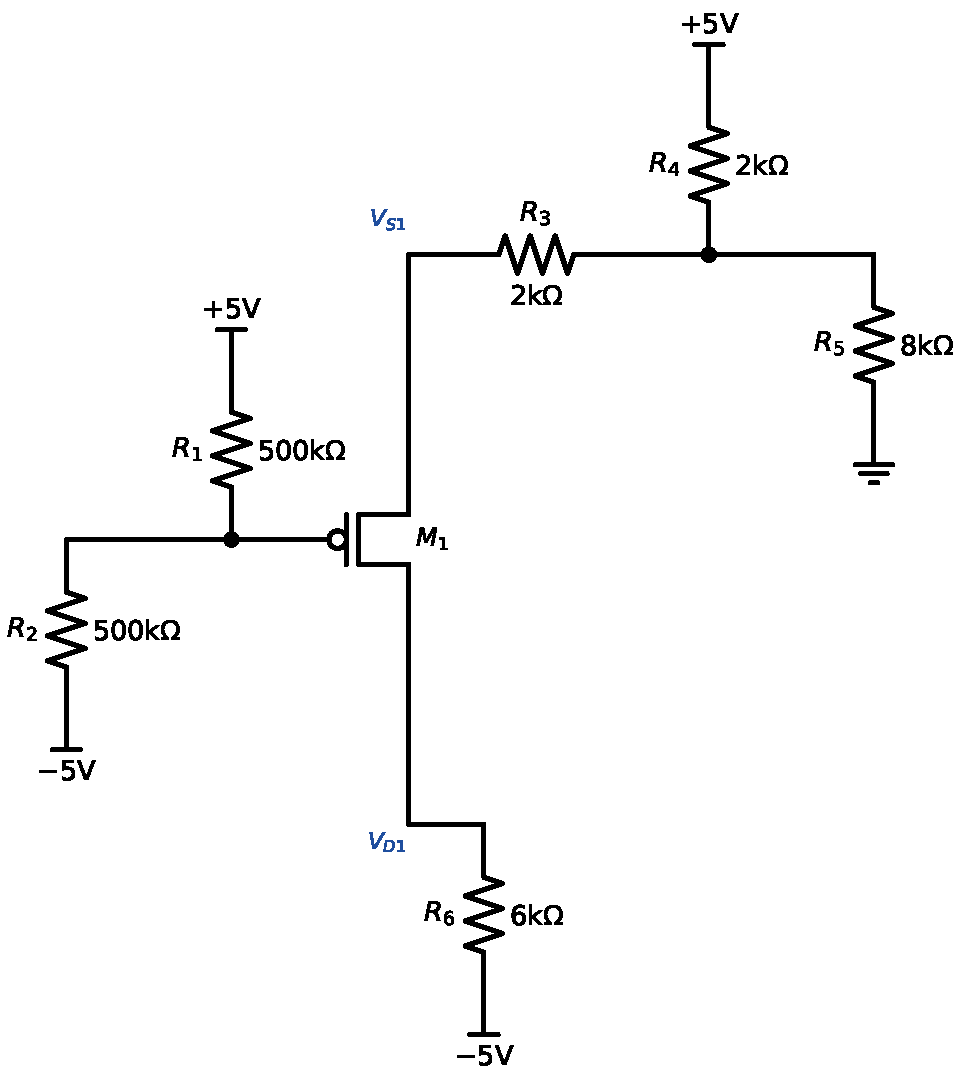
\includegraphics[width=0.9\linewidth,height=6cm,keepaspectratio]{p02_circuit}\end{center}
\solstep{1}{Why Thevenin}Plain KCL would need all 4 unknown node voltages at once, and the transistor equation is quadratic, so the elimination by hand is long. But each transistor touches every resistor network at a single terminal, and the gate draws no current. So every network can be replaced by its Thevenin pair $(V_{th}, R_{th})$ (tool T5), computed with the transistor removed --- 3 small networks, each a chain of dividers. What is left is one loop per transistor with a single quadratic.
\solstep{2}{Transistor $M_{1}$}\emph{Gate network} (seen from the gate of $M_{1}$, transistor removed). At $V_{G1}$ combine in parallel $R_{1}$ to $5$, $R_{2}$ to $(-5)$ (Millman): \[V_{th} = \frac{\sum V_k/R_k}{\sum 1/R_k} = 0\,\mathrm{V},\qquad R_{th} = 500\,\mathrm{k}\Omega \| 500\,\mathrm{k}\Omega = 250\,\mathrm{k}\Omega\] No current flows into the gate, so only $V_{th}$ matters: $V_{G1} = V_{th,G1} = 0\,\mathrm{V}$.

\emph{Source network} (seen from the source of $M_{1}$). At $V_{x1}$ combine in parallel $R_{4}$ to $5$, $R_{5}$ to $0$ (Millman): \[V_{th} = \frac{\sum V_k/R_k}{\sum 1/R_k} = 4\,\mathrm{V},\qquad R_{th} = 2\,\mathrm{k}\Omega \| 8\,\mathrm{k}\Omega = 1.6\,\mathrm{k}\Omega\] Through $R_{3}$ in series: $R_{th}$ grows by $R_{3}$: $(V_{th}, R_{th}) = (4\,\mathrm{V},\ 3.6\,\mathrm{k}\Omega)$.

\emph{Drain network} (seen from the drain of $M_{1}$). Start at $V_{D1}$: only $R_{6}$ to $(-5)$, i.e. $(V_{th}, R_{th}) = (-5\,\mathrm{V},\ 6\,\mathrm{k}\Omega)$.

With the networks replaced, $M_{1}$ sees one loop: gate at $0\,\mathrm{V}$, source through $R_{th,S1} = 3.6\,\mathrm{k}\Omega$ to $V_{th,S1} = 4\,\mathrm{V}$. KVL (assume $M_{1}$ active):\[V_{th,S1} - V_{G1} = 4 = V_{SG1} + R_{th,S1}I_{D1},\qquad I_{D1} = \frac{850\,\mu }{2}(V_{SG1} - 1.3)^2\]\[1.53V_{SG1}^2 - 2.978V_{SG1} - 1.414 = 0 \;\Rightarrow\; V_{SG1} = -0.3948\ \text{or}\ 2.341\,\mathrm{V}\]The root $-0.395$\,V is below $|V_t| = 1.3$\,V (the transistor would be off), so $V_{SG1} = 2.341$\,V. So $I_{D1} = 461\,\mu \mathrm{A}$.

Terminal voltages: $V_{S1} = V_{G1} + V_{SG1} = 2.34\,\mathrm{V}$, $V_{D1} = V_{th,D1} + R_{th,D1}I_{D1} = -5 + 6\,\mathrm{k}\times461\,\mu \mathrm{A} = -2.24\,\mathrm{V}$.

Check: $V_{SD1} = 4.577$\,V $\ge V_{ov1} = 1.04$\,V: $M_{1}$ is active \checkmark
\solstep{3}{Equivalent circuit}With every network replaced by its Thevenin pair the circuit is just this (the solution above is the analysis of this circuit):\begin{center}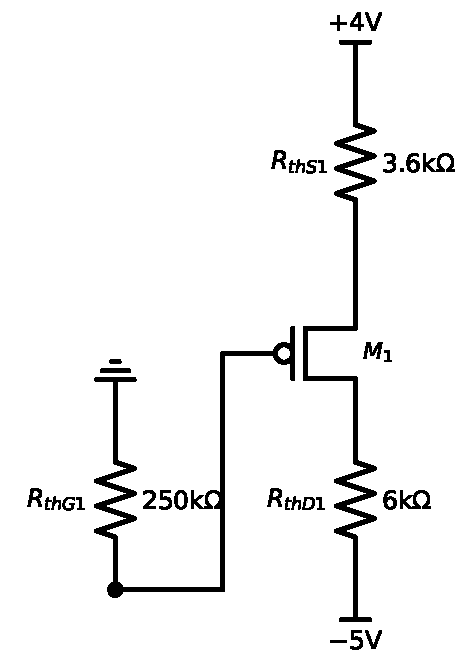
\includegraphics[width=0.6\linewidth,height=5cm,keepaspectratio]{p02_equivalent}\end{center}

A full nodal solve of the original circuit (all 4 node voltages) gives the same currents.
\begin{ansbox}
$I_{D1} = 461\,\mu \mathrm{A}$, $V_{S1} = 2.34\,\mathrm{V}$, $V_{D1} = -2.24\,\mathrm{V}$\\[2pt] all transistors active.
\end{ansbox}

\newpage
\subsection*{Solution 5F.3 \hfill Easy}
\begin{center}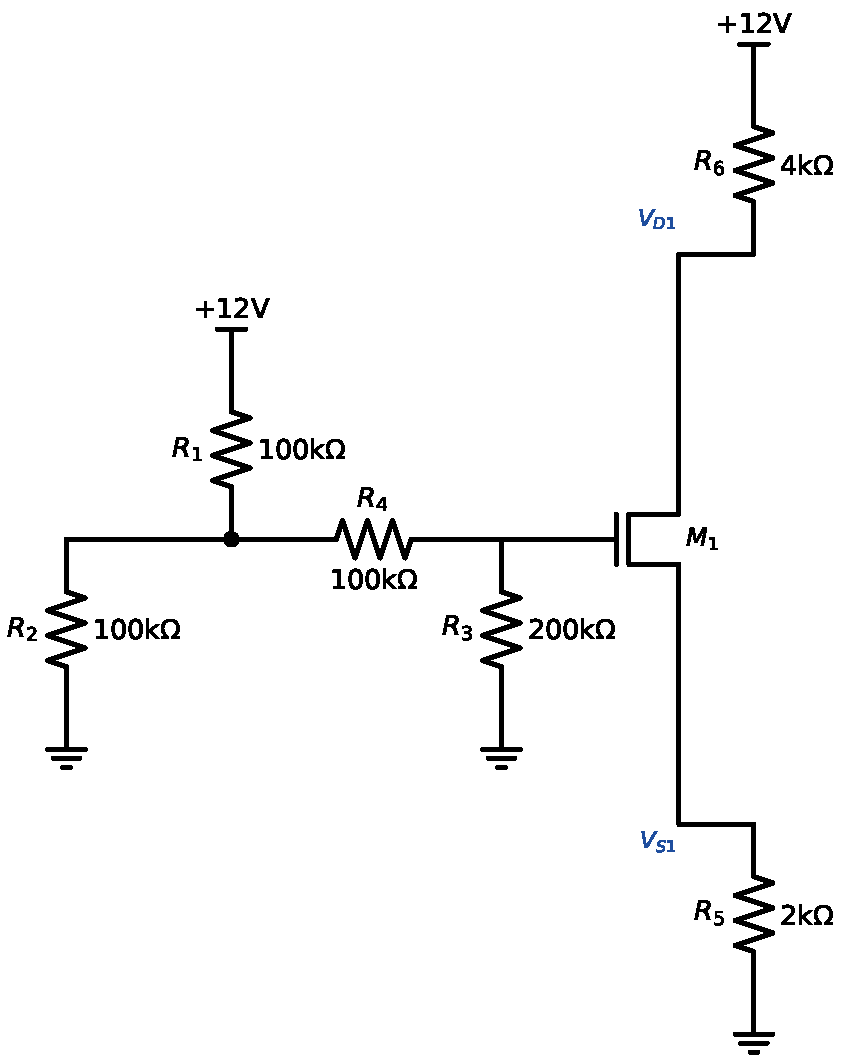
\includegraphics[width=0.9\linewidth,height=6cm,keepaspectratio]{p03_circuit}\end{center}
\solstep{1}{Why Thevenin}Plain KCL would need all 4 unknown node voltages at once, and the transistor equation is quadratic, so the elimination by hand is long. But each transistor touches every resistor network at a single terminal, and the gate draws no current. So every network can be replaced by its Thevenin pair $(V_{th}, R_{th})$ (tool T5), computed with the transistor removed --- 3 small networks, each a chain of dividers. What is left is one loop per transistor with a single quadratic.
\solstep{2}{Transistor $M_{1}$}\emph{Gate network} (seen from the gate of $M_{1}$, transistor removed). At $V_{x1}$ combine in parallel $R_{1}$ to $12$, $R_{2}$ to $0$ (Millman): \[V_{th} = \frac{\sum V_k/R_k}{\sum 1/R_k} = 6\,\mathrm{V},\qquad R_{th} = 100\,\mathrm{k}\Omega \| 100\,\mathrm{k}\Omega = 50\,\mathrm{k}\Omega\] Through $R_{4}$ in series: $R_{th}$ grows by $R_{4}$: $(V_{th}, R_{th}) = (6\,\mathrm{V},\ 150\,\mathrm{k}\Omega)$. At $V_{G1}$ combine in parallel the part already reduced, $R_{3}$ to $0$ (Millman): \[V_{th} = \frac{\sum V_k/R_k}{\sum 1/R_k} = 3.429\,\mathrm{V},\qquad R_{th} = 150\,\mathrm{k}\Omega \| 200\,\mathrm{k}\Omega = 85.7\,\mathrm{k}\Omega\] No current flows into the gate, so only $V_{th}$ matters: $V_{G1} = V_{th,G1} = 3.43\,\mathrm{V}$.

\emph{Source network} (seen from the source of $M_{1}$). Start at $V_{S1}$: only $R_{5}$ to $0$, i.e. $(V_{th}, R_{th}) = (0\,\mathrm{V},\ 2\,\mathrm{k}\Omega)$.

\emph{Drain network} (seen from the drain of $M_{1}$). Start at $V_{D1}$: only $R_{6}$ to $12$, i.e. $(V_{th}, R_{th}) = (12\,\mathrm{V},\ 4\,\mathrm{k}\Omega)$.

With the networks replaced, $M_{1}$ sees one loop: gate at $3.43\,\mathrm{V}$, source through $R_{th,S1} = 2\,\mathrm{k}\Omega$ to $V_{th,S1} = 0\,\mathrm{V}$. KVL (assume $M_{1}$ active):\[V_{G1} - V_{th,S1} = 3.429 = V_{GS1} + R_{th,S1}I_{D1},\qquad I_{D1} = \frac{1.1\,\mathrm{m}}{2}(V_{GS1} - 1.4)^2\]\[1.1V_{GS1}^2 - 2.08V_{GS1} - 1.273 = 0 \;\Rightarrow\; V_{GS1} = -0.4866\ \text{or}\ 2.378\,\mathrm{V}\]The root $-0.487$\,V is below $|V_t| = 1.4$\,V (the transistor would be off), so $V_{GS1} = 2.378$\,V. So $I_{D1} = 526\,\mu \mathrm{A}$.

Terminal voltages: $V_{S1} = V_{G1} - V_{GS1} = 1.05\,\mathrm{V}$, $V_{D1} = V_{th,D1} - R_{th,D1}I_{D1} = 12 - 4\,\mathrm{k}\times526\,\mu \mathrm{A} = 9.9\,\mathrm{V}$.

Check: $V_{DS1} = 8.847$\,V $\ge V_{ov1} = 0.978$\,V: $M_{1}$ is active \checkmark
\solstep{3}{Equivalent circuit}With every network replaced by its Thevenin pair the circuit is just this (the solution above is the analysis of this circuit):\begin{center}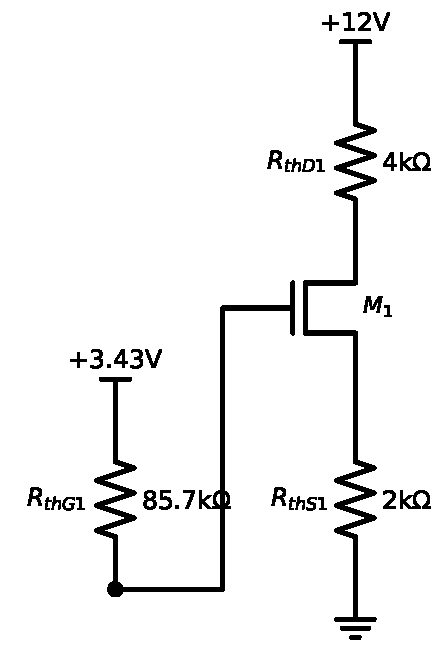
\includegraphics[width=0.6\linewidth,height=5cm,keepaspectratio]{p03_equivalent}\end{center}

A full nodal solve of the original circuit (all 4 node voltages) gives the same currents.
\begin{ansbox}
$I_{D1} = 526\,\mu \mathrm{A}$, $V_{S1} = 1.05\,\mathrm{V}$, $V_{D1} = 9.9\,\mathrm{V}$\\[2pt] all transistors active.
\end{ansbox}

\newpage
\subsection*{Solution 5F.4 \hfill Easy}
\begin{center}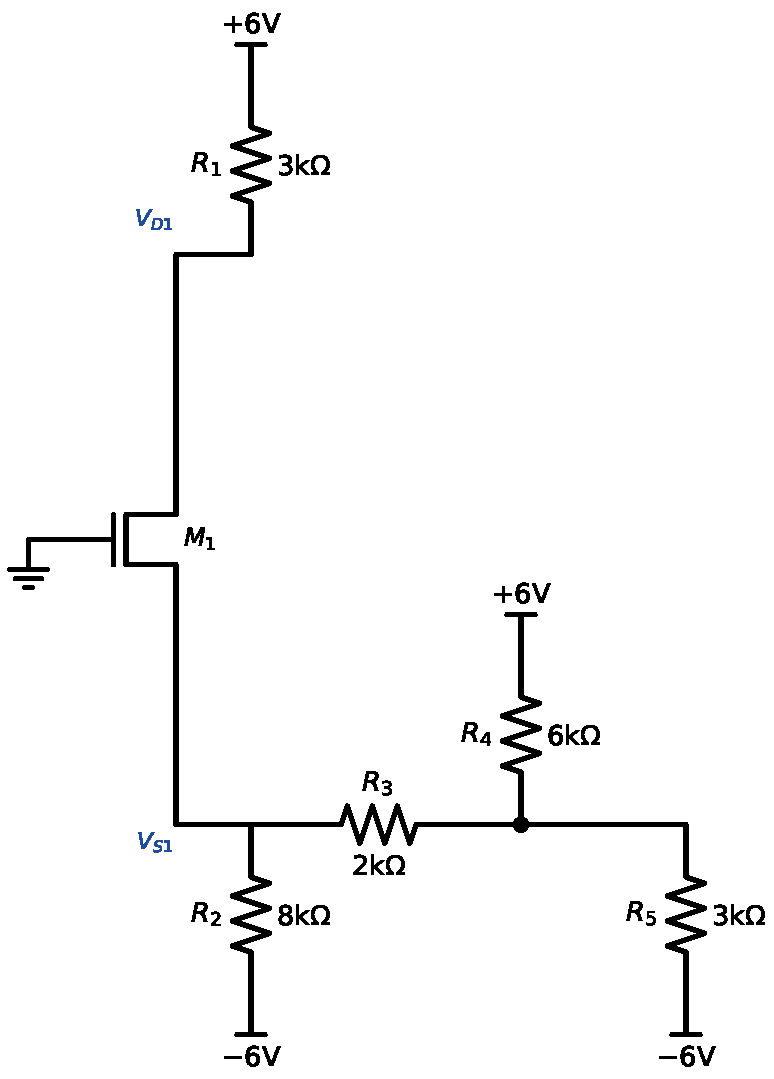
\includegraphics[width=0.9\linewidth,height=6cm,keepaspectratio]{p04_circuit}\end{center}
\solstep{1}{Why Thevenin}Plain KCL would need all 3 unknown node voltages at once, and the transistor equation is quadratic, so the elimination by hand is long. But each transistor touches every resistor network at a single terminal, and the gate draws no current. So every network can be replaced by its Thevenin pair $(V_{th}, R_{th})$ (tool T5), computed with the transistor removed --- 2 small networks, each a chain of dividers. What is left is one loop per transistor with a single quadratic.
\solstep{2}{Transistor $M_{1}$}\emph{Source network} (seen from the source of $M_{1}$). At $V_{x1}$ combine in parallel $R_{4}$ to $6$, $R_{5}$ to $(-6)$ (Millman): \[V_{th} = \frac{\sum V_k/R_k}{\sum 1/R_k} = -2\,\mathrm{V},\qquad R_{th} = 6\,\mathrm{k}\Omega \| 3\,\mathrm{k}\Omega = 2\,\mathrm{k}\Omega\] Through $R_{3}$ in series: $R_{th}$ grows by $R_{3}$: $(V_{th}, R_{th}) = (-2\,\mathrm{V},\ 4\,\mathrm{k}\Omega)$. At $V_{S1}$ combine in parallel the part already reduced, $R_{2}$ to $(-6)$ (Millman): \[V_{th} = \frac{\sum V_k/R_k}{\sum 1/R_k} = -3.333\,\mathrm{V},\qquad R_{th} = 4\,\mathrm{k}\Omega \| 8\,\mathrm{k}\Omega = 2.67\,\mathrm{k}\Omega\]

\emph{Drain network} (seen from the drain of $M_{1}$). Start at $V_{D1}$: only $R_{1}$ to $6$, i.e. $(V_{th}, R_{th}) = (6\,\mathrm{V},\ 3\,\mathrm{k}\Omega)$.

With the networks replaced, $M_{1}$ sees one loop: gate at $0\,\mathrm{V}$, source through $R_{th,S1} = 2.67\,\mathrm{k}\Omega$ to $V_{th,S1} = -3.33\,\mathrm{V}$. KVL (assume $M_{1}$ active):\[V_{G1} - V_{th,S1} = 3.333 = V_{GS1} + R_{th,S1}I_{D1},\qquad I_{D1} = \frac{1.1\,\mathrm{m}}{2}(V_{GS1} - 1.4)^2\]\[1.467V_{GS1}^2 - 3.107V_{GS1} - 0.4587 = 0 \;\Rightarrow\; V_{GS1} = -0.1386\ \text{or}\ 2.257\,\mathrm{V}\]The root $-0.139$\,V is below $|V_t| = 1.4$\,V (the transistor would be off), so $V_{GS1} = 2.257$\,V. So $I_{D1} = 404\,\mu \mathrm{A}$.

Terminal voltages: $V_{S1} = 0 - V_{GS1} = -2.26\,\mathrm{V}$, $V_{D1} = V_{th,D1} - R_{th,D1}I_{D1} = 6 - 3\,\mathrm{k}\times404\,\mu \mathrm{A} = 4.79\,\mathrm{V}$.

Check: $V_{DS1} = 7.046$\,V $\ge V_{ov1} = 0.857$\,V: $M_{1}$ is active \checkmark
\solstep{3}{Equivalent circuit}With every network replaced by its Thevenin pair the circuit is just this (the solution above is the analysis of this circuit):\begin{center}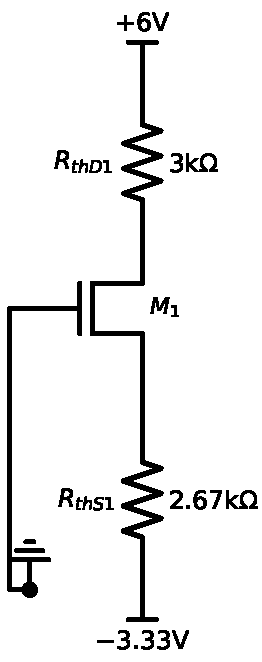
\includegraphics[width=0.6\linewidth,height=5cm,keepaspectratio]{p04_equivalent}\end{center}

A full nodal solve of the original circuit (all 3 node voltages) gives the same currents.
\begin{ansbox}
$I_{D1} = 404\,\mu \mathrm{A}$, $V_{S1} = -2.26\,\mathrm{V}$, $V_{D1} = 4.79\,\mathrm{V}$\\[2pt] all transistors active.
\end{ansbox}

\newpage
\subsection*{Solution 5F.5 \hfill Easy}
\begin{center}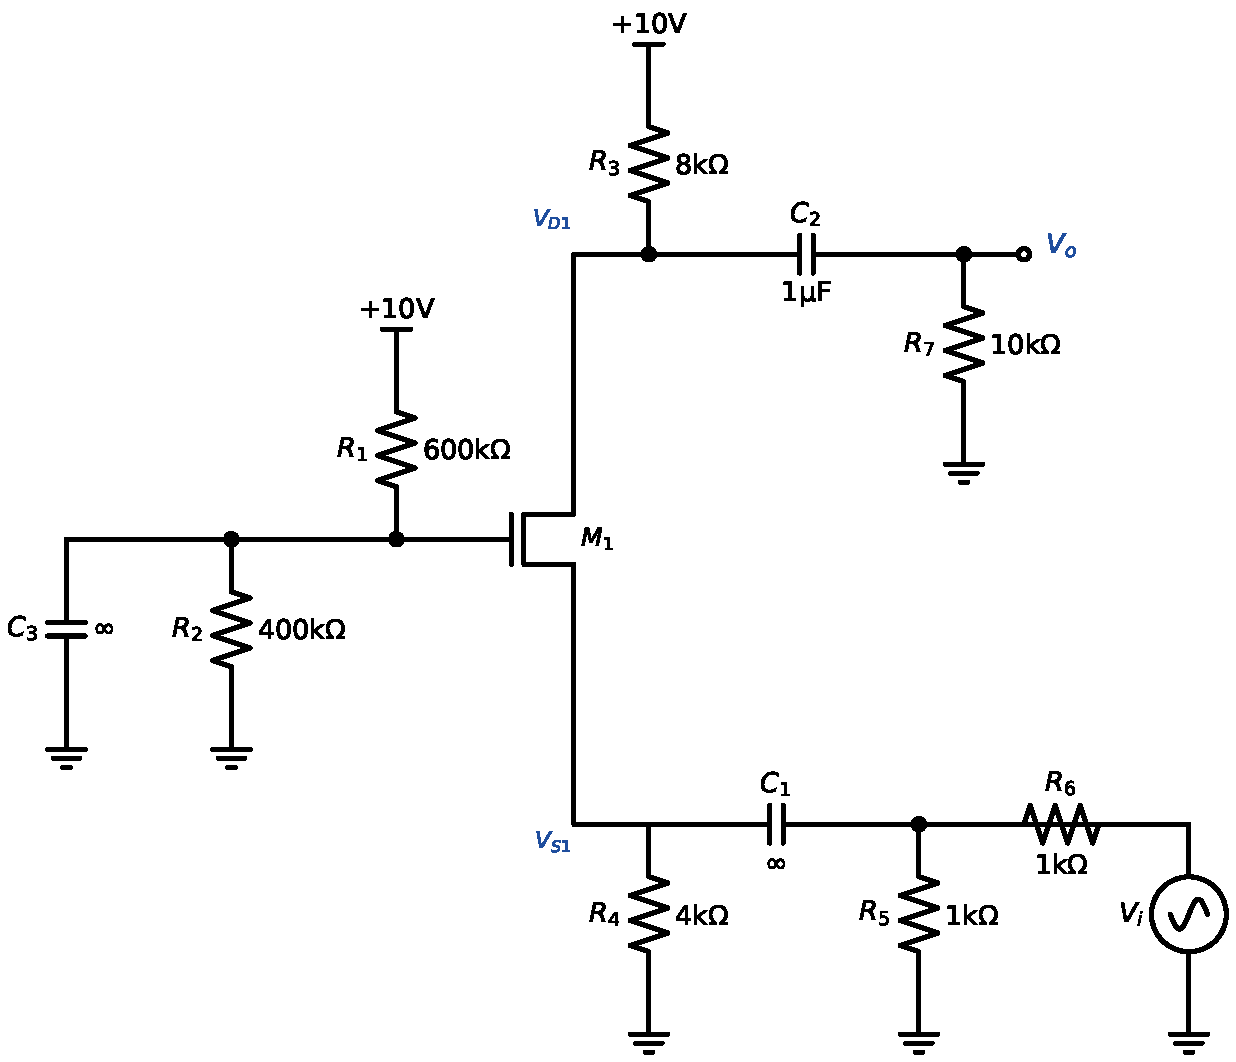
\includegraphics[width=0.9\linewidth,height=6cm,keepaspectratio]{p05_circuit}\end{center}
\solstep{1}{DC currents and transconductances}The DC drain currents are given: $I_{D1} = 429\,\mu \mathrm{A}$. For AC every supply is ground and every ``$\infty$'' capacitor is a short. Transconductances (tool T4):\begin{align*}
g_{m1} &= k_{1}V_{ov1} = \sqrt{2k_{1}I_{D1}} = \sqrt{2\cdot1.1\,\mathrm{m}\mathrm{A/V^2}\cdot429\,\mu \mathrm{A}} = 972\,\mu \mathrm{A/V},\qquad \frac{1}{g_{m1}} = 1.03\,\mathrm{k}\Omega\quad(V_{ov1} = 0.883\,\mathrm{V})
\end{align*}

\solstep{2}{Thevenin equivalent of the input network}Between $v_i$ and the source of $M_{1}$ there is a whole network (with KCL: one equation per node, in $s$). The transistor touches it only at its source, so replace it by its Thevenin pair $(V_{th}(s), Z_{th}(s))$ seen from there (tool T5), marching from the far end: At $V_{x1}$ combine in parallel $R_{5}$ to $0$, $R_{6}$ to $v_i$ (Millman): \[V_{th} = \frac{\sum V_k/Z_k}{\sum 1/Z_k} = 0.5\,v_i,\qquad Z_{th} = 1\,\mathrm{k}\Omega \| 1\,\mathrm{k}\Omega = 500\,\Omega\] $C_{1}$ is a short ($\infty$ capacitor): the pair is unchanged. At $V_{S1}$ combine in parallel the part already reduced, $R_{4}$ to $0$ (Millman): \[V_{th} = \frac{\sum V_k/Z_k}{\sum 1/Z_k} = 0.444\,v_i,\qquad Z_{th} = 500\,\Omega \| 4\,\mathrm{k}\Omega = 444\,\Omega\] The source of the common-gate stage presents $1/g_{m1} = 1.03\,\mathrm{k}\Omega$ to this Thevenin source, a voltage divider: \[\frac{v_{s1}}{v_i} = \frac{V_{th}}{v_i}\cdot\frac{1/g_{m1}}{Z_{th} + 1/g_{m1}} = 0.31\]
\solstep{3}{Rest of the signal path}Input resistance of every stage, from the last back to the first (each one loads the stage before it):\begin{align*}
R_{i1} &= Z_{source,1} = \frac{1}{g_{m1}} = 1.03\,\mathrm{k}\Omega\quad\text{(common gate)}
\end{align*}
Multiply the node-to-node gains along the signal path (tool T4):\[
H(s) = \frac{v_{d1}}{v_{s1}}\cdot\frac{v_o}{v_{d1}}
\]
\begin{align*}
\frac{v_{d1}}{v_{s1}} &= \frac{Z_{D1}}{1/g_{m1}},\quad Z_{D1} = R_{3} \parallel \left(\frac{1}{sC_{2}} + R_{7}\right)\ \Rightarrow\ \dfrac{4.32\,s + 432}{s + 55.6} \\
\frac{v_o}{v_{d1}} &= \frac{R_{7}}{\frac{1}{sC_{2}} + R_{7}} = \dfrac{s}{s + 100}
\end{align*}

\solstep{4}{Transfer function}Multiply and simplify:\[
H(s) = \dfrac{1.34\,s}{s + 55.6}
\]

\solstep{5}{Standard (Bode-ready) form}Find the roots. Every root $s=-p$ of the denominator is a \emph{pole}, every root $s=-z$ of the numerator is a \emph{zero}; $|p|$ and $|z|$ are the corner frequencies (rad/s).
\begin{itemize}[leftmargin=*,itemsep=2pt]
\item Numerator: it has the factor $s$ $\Rightarrow$ 1 zero at $s=0$.
\item Denominator: $s + 55.6$; $s + 55.6 = 0 \Rightarrow s = -55.6$.
\end{itemize}

Factored form (leading coefficient in front):
\[
H(s) = 1.34\,\dfrac{s}{(s+55.6)}
\]

Bode-ready form: rewrite every $(s+p) = p\left(1+\frac{s}{p}\right)$ and $(s+z) = z\left(1+\frac{s}{z}\right)$, and collect all constants into $K$. Each $s$ in the numerator is paired with one of the \emph{lowest} poles as $\frac{s}{s+p}$ (that factor is $\approx 1$ above $p$). Then every factor except $K$ is $\approx 1$ inside the pass-band:
\[
H(s) = 1.34\,\dfrac{s}{s+2\pi\cdot 8.84},\qquad K = 1.34
\]

\begin{center}\renewcommand{\arraystretch}{1.35}
\begin{tabular}{cccc}
\toprule
type & $\omega_c$ (rad/s) & $f_c=\omega_c/2\pi$ & slope change \\
\midrule
pole & $55.6$ & 8.84 Hz & $-20$ dB/dec \\
\bottomrule
\end{tabular}\end{center}

\solstep{6}{Magnitude Bode plot}Below every corner $|H(s)|\approx 0.0241\,s$, so the plot starts with a slope of $+20$\,dB/dec. Then, moving right, each pole bends the line down by 20\,dB/dec and each zero bends it up by 20\,dB/dec (tool T6):
\begin{center}\renewcommand{\arraystretch}{1.35}
\begin{tabular}{lcl}
\toprule
frequency range & slope & asymptote level \\
\midrule
$f<$ 8.84 Hz & $+20$ dB/dec & 2.55 dB at end \\
$f>$ 8.84 Hz & $0$ dB/dec (flat) & 2.55 dB at start \\
\bottomrule
\end{tabular}\end{center}

The flat (pass-band) level is $20\log_{10}|K| = 20\log_{10}1.34 = 2.55$\,dB.
\begin{center}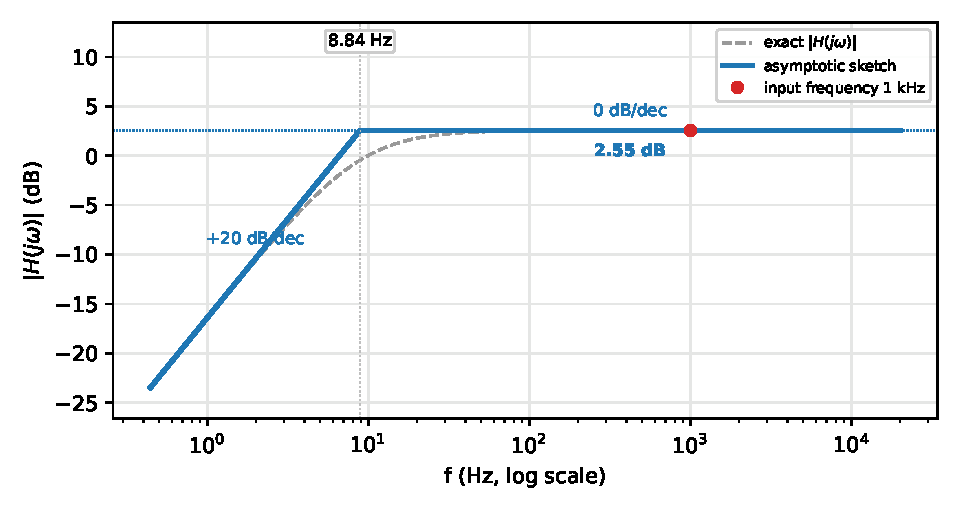
\includegraphics[width=0.78\linewidth,height=6.5cm,keepaspectratio]{p05_bode}\end{center}

{\small Blue: the straight-line sketch you are expected to draw. Dashed grey: the exact curve (about 3\,dB below the corner of an isolated pole). Red dot: the input frequency of Step 7.}
\solstep{7}{Steady-state output}The input is $V_i(t) = 0.01\sin\left(2\pi\cdot 1000\,t\right)$, so $\omega_{in} = 2\pi\cdot 1000 = 6280$\,rad/s. Put $s=j\omega_{in}$ in each factor (tool T5): magnitudes multiply, angles add.
{\small Rules: $\left|\frac{s}{s+p}\right| = \frac{\omega}{\sqrt{\omega^2+p^2}}$, $\angle = \frac{\pi}{2}-\tan^{-1}\frac{\omega}{p}$;\quad $\left|\frac{1}{1+s/p}\right| = \frac{1}{\sqrt{1+(\omega/p)^2}}$, $\angle = -\tan^{-1}\frac{\omega}{p}$;\quad $\left|1+\frac{s}{z}\right| = \sqrt{1+(\omega/z)^2}$, $\angle = \tan^{-1}\frac{\omega}{z}$;\quad a negative $K$ adds $-\pi$.}
\begin{center}\renewcommand{\arraystretch}{1.35}
\begin{tabular}{ccc}
\toprule
factor & magnitude & angle (rad) \\
\midrule
$1.34$ & $1.34$ & $0$ \\
$\rule[-1.1em]{0pt}{2.8em}\dfrac{s}{s+2\pi\cdot 8.84}$ & $1$ & $0.00884$ \\
\textbf{total} & $\mathbf{1.34}$ (product) & $\mathbf{0.00884}$ (sum) \\
\bottomrule
\end{tabular}\end{center}

\begin{align*}
|H(j\omega_{in})| &= 1.34, \qquad \angle H(j\omega_{in}) = 0.00884\ \mathrm{rad} \\
v_{o,ac}(t) &= 1.34\times 0.01\,\sin\left(2\pi\cdot 1000\,t + 0.00884\right) = 0.0134\,\sin\left(2\pi\cdot 1000\,t + 0.00884\right)
\end{align*}

\[
\boxed{V_o(t) = 0.0134\,\sin\left(2\pi\cdot 1000\,t + 0.00884\right)\ \mathrm{V}}
\]

\begin{ansbox}
$H(s) = 1.34\,\dfrac{s}{s+2\pi\cdot 8.84}$\quad (corners: 8.84 Hz)\\[4pt]
$V_o(t) = 0.0134\,\sin\left(2\pi\cdot 1000\,t + 0.00884\right)\ \mathrm{V}$
\end{ansbox}

\newpage
\subsection*{Solution 5F.6 \hfill Easy}
\begin{center}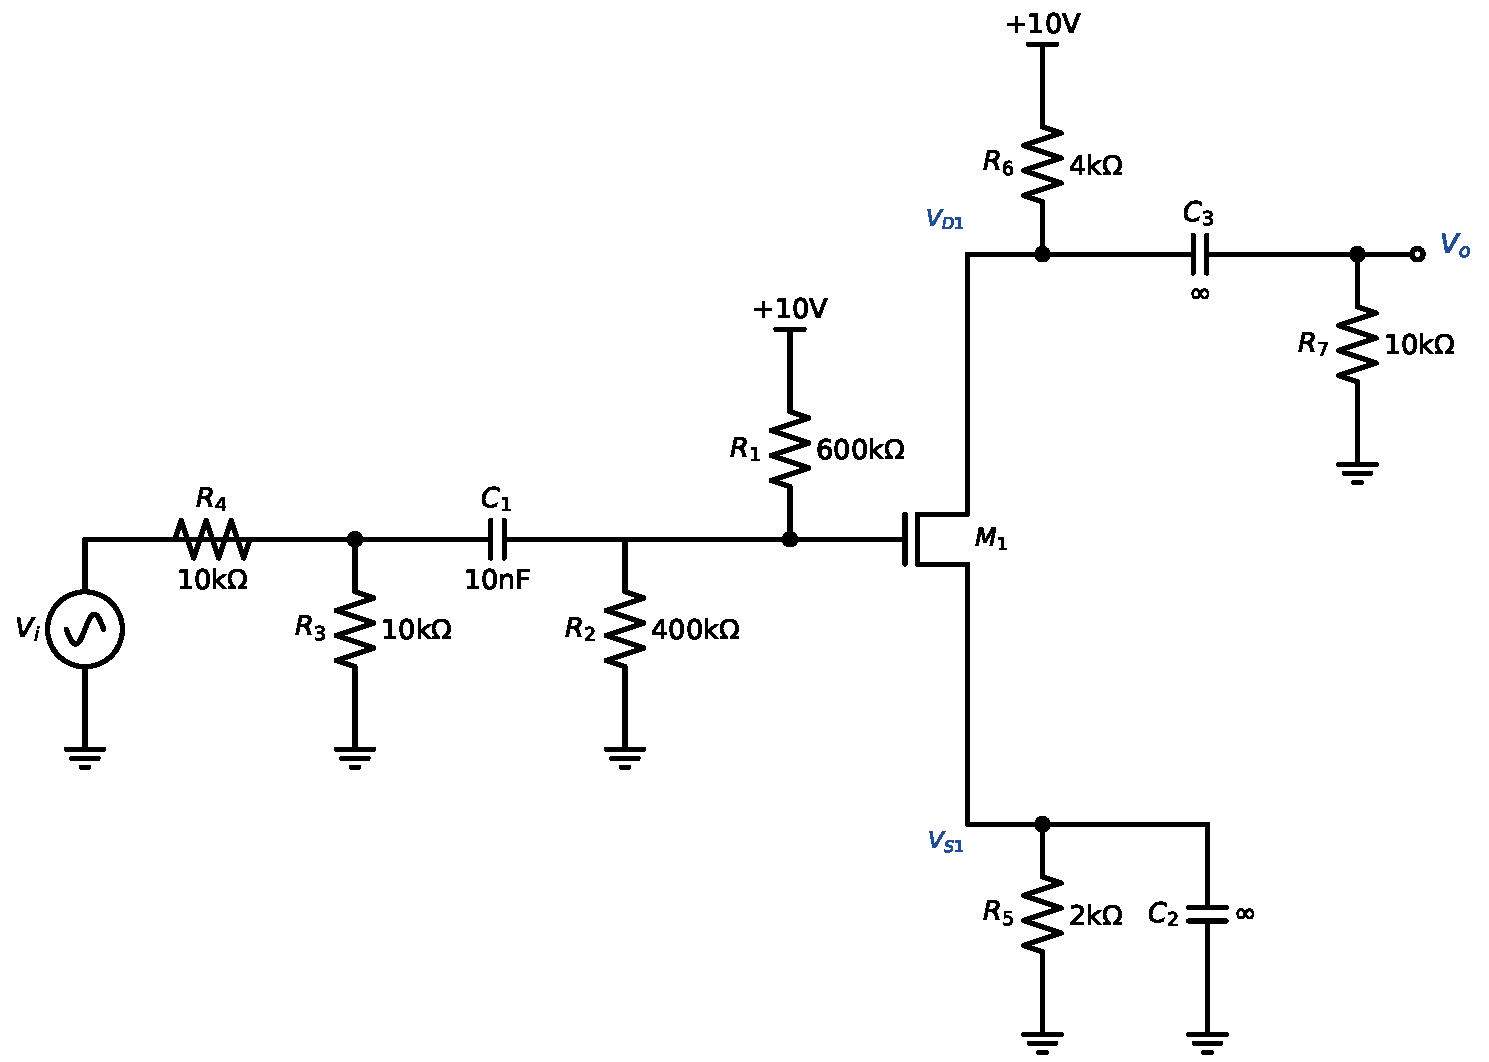
\includegraphics[width=0.9\linewidth,height=6cm,keepaspectratio]{p06_circuit}\end{center}
\solstep{1}{DC currents and transconductances}The DC drain currents are given: $I_{D1} = 726\,\mu \mathrm{A}$. For AC every supply is ground and every ``$\infty$'' capacitor is a short. Transconductances (tool T4):\begin{align*}
g_{m1} &= k_{1}V_{ov1} = \sqrt{2k_{1}I_{D1}} = \sqrt{2\cdot1.1\,\mathrm{m}\mathrm{A/V^2}\cdot726\,\mu \mathrm{A}} = 1.26\,\mathrm{m}\mathrm{A/V},\qquad \frac{1}{g_{m1}} = 791\,\Omega\quad(V_{ov1} = 1.15\,\mathrm{V})
\end{align*}

\solstep{2}{Thevenin equivalent of the input network}Between $v_i$ and the gate of $M_{1}$ there is a whole network (with KCL: one equation per node, in $s$). The transistor touches it only at its gate, so replace it by its Thevenin pair $(V_{th}(s), Z_{th}(s))$ seen from there (tool T5), marching from the far end: At $V_{x1}$ combine in parallel $R_{3}$ to $0$, $R_{4}$ to $v_i$ (Millman): \[V_{th} = \frac{\sum V_k/Z_k}{\sum 1/Z_k} = 0.5\,v_i,\qquad Z_{th} = 10\,\mathrm{k}\Omega \| 10\,\mathrm{k}\Omega = 5\,\mathrm{k}\Omega\] Through $C_{1}$ in series: $Z_{th}$ grows by $\frac{1}{sC_{1}}$: $(V_{th}, Z_{th}) = (0.5\,v_i,\ \dfrac{5000\,s + 10^{8}}{s})$. At $V_{G1}$ combine in parallel the part already reduced, $R_{1}$ to $0$, $R_{2}$ to $0$ (Millman): \[V_{th} = \frac{\sum V_k/Z_k}{\sum 1/Z_k} = \dfrac{0.49\,s}{s + 408}\,v_i,\qquad Z_{th} = \dfrac{5000\,s + 10^{8}}{s} \| 600\,\mathrm{k}\Omega \| 400\,\mathrm{k}\Omega = \dfrac{4900\,s + 9.8\times 10^{7}}{s + 408}\] No current flows into the gate, so $Z_{th}$ plays no role: \[\frac{v_{g1}}{v_i} = \frac{V_{th}}{v_i} = \dfrac{0.49\,s}{s + 408}\]
\solstep{3}{Rest of the signal path}Input resistance of every stage, from the last back to the first (each one loads the stage before it):\begin{align*}
R_{i1} &= Z_{gate,1} = \infty\quad\text{(input at the gate: it loads nothing)}
\end{align*}
Multiply the node-to-node gains along the signal path (tool T4):\[
H(s) = \frac{v_{d1}}{v_{g1}}
\]
\begin{align*}
\frac{v_{d1}}{v_{g1}} &= -\frac{Z_{D1}}{1/g_{m1} + Z_{S1}},\quad Z_{D1} = R_{6} \parallel R_{7},\ Z_{S1} = 0\ \Rightarrow\ -3.61
\end{align*}

\solstep{4}{Transfer function}Multiply and simplify:\[
H(s) = \dfrac{-1.77\,s}{s + 408}
\]

\solstep{5}{Standard (Bode-ready) form}Find the roots. Every root $s=-p$ of the denominator is a \emph{pole}, every root $s=-z$ of the numerator is a \emph{zero}; $|p|$ and $|z|$ are the corner frequencies (rad/s).
\begin{itemize}[leftmargin=*,itemsep=2pt]
\item Numerator: it has the factor $s$ $\Rightarrow$ 1 zero at $s=0$.
\item Denominator: $s + 408$; $s + 408 = 0 \Rightarrow s = -408$.
\end{itemize}

Factored form (leading coefficient in front):
\[
H(s) = -1.77\,\dfrac{s}{(s+408)}
\]

Bode-ready form: rewrite every $(s+p) = p\left(1+\frac{s}{p}\right)$ and $(s+z) = z\left(1+\frac{s}{z}\right)$, and collect all constants into $K$. Each $s$ in the numerator is paired with one of the \emph{lowest} poles as $\frac{s}{s+p}$ (that factor is $\approx 1$ above $p$). Then every factor except $K$ is $\approx 1$ inside the pass-band:
\[
H(s) = -1.77\,\dfrac{s}{s+2\pi\cdot 65},\qquad K = -1.77
\]

\begin{center}\renewcommand{\arraystretch}{1.35}
\begin{tabular}{cccc}
\toprule
type & $\omega_c$ (rad/s) & $f_c=\omega_c/2\pi$ & slope change \\
\midrule
pole & $408$ & 65 Hz & $-20$ dB/dec \\
\bottomrule
\end{tabular}\end{center}

\solstep{6}{Magnitude Bode plot}Below every corner $|H(s)|\approx 0.00433\,s$, so the plot starts with a slope of $+20$\,dB/dec. Then, moving right, each pole bends the line down by 20\,dB/dec and each zero bends it up by 20\,dB/dec (tool T6):
\begin{center}\renewcommand{\arraystretch}{1.35}
\begin{tabular}{lcl}
\toprule
frequency range & slope & asymptote level \\
\midrule
$f<$ 65 Hz & $+20$ dB/dec & 4.95 dB at end \\
$f>$ 65 Hz & $0$ dB/dec (flat) & 4.95 dB at start \\
\bottomrule
\end{tabular}\end{center}

The flat (pass-band) level is $20\log_{10}|K| = 20\log_{10}1.77 = 4.95$\,dB.
\begin{center}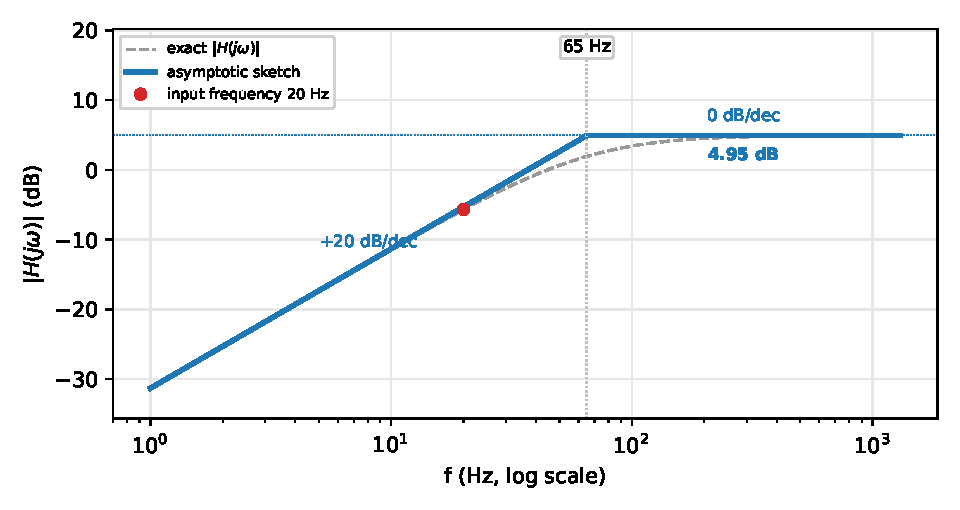
\includegraphics[width=0.78\linewidth,height=6.5cm,keepaspectratio]{p06_bode}\end{center}

{\small Blue: the straight-line sketch you are expected to draw. Dashed grey: the exact curve (about 3\,dB below the corner of an isolated pole). Red dot: the input frequency of Step 7.}
\solstep{7}{Steady-state output}The input is $V_i(t) = 0.02\sin\left(2\pi\cdot 20\,t\right)$, so $\omega_{in} = 2\pi\cdot 20 = 126$\,rad/s. Put $s=j\omega_{in}$ in each factor (tool T5): magnitudes multiply, angles add.
{\small Rules: $\left|\frac{s}{s+p}\right| = \frac{\omega}{\sqrt{\omega^2+p^2}}$, $\angle = \frac{\pi}{2}-\tan^{-1}\frac{\omega}{p}$;\quad $\left|\frac{1}{1+s/p}\right| = \frac{1}{\sqrt{1+(\omega/p)^2}}$, $\angle = -\tan^{-1}\frac{\omega}{p}$;\quad $\left|1+\frac{s}{z}\right| = \sqrt{1+(\omega/z)^2}$, $\angle = \tan^{-1}\frac{\omega}{z}$;\quad a negative $K$ adds $-\pi$.}
\begin{center}\renewcommand{\arraystretch}{1.35}
\begin{tabular}{ccc}
\toprule
factor & magnitude & angle (rad) \\
\midrule
$-1.77$ & $1.768$ & $-3.14$ \\
$\rule[-1.1em]{0pt}{2.8em}\dfrac{s}{s+2\pi\cdot 65}$ & $0.2942$ & $1.27$ \\
\textbf{total} & $\mathbf{0.5203}$ (product) & $\mathbf{-1.87}$ (sum) \\
\bottomrule
\end{tabular}\end{center}

\begin{align*}
|H(j\omega_{in})| &= 0.52, \qquad \angle H(j\omega_{in}) = -1.87\ \mathrm{rad} \\
v_{o,ac}(t) &= 0.52\times 0.02\,\sin\left(2\pi\cdot 20\,t - 1.87\right) = 0.0104\,\sin\left(2\pi\cdot 20\,t - 1.87\right)
\end{align*}

\[
\boxed{V_o(t) = 0.0104\,\sin\left(2\pi\cdot 20\,t - 1.87\right)\ \mathrm{V}}
\]

\begin{ansbox}
$H(s) = -1.77\,\dfrac{s}{s+2\pi\cdot 65}$\quad (corners: 65 Hz)\\[4pt]
$V_o(t) = 0.0104\,\sin\left(2\pi\cdot 20\,t - 1.87\right)\ \mathrm{V}$
\end{ansbox}

\newpage
\subsection*{Solution 5F.7 \hfill Medium}
\begin{center}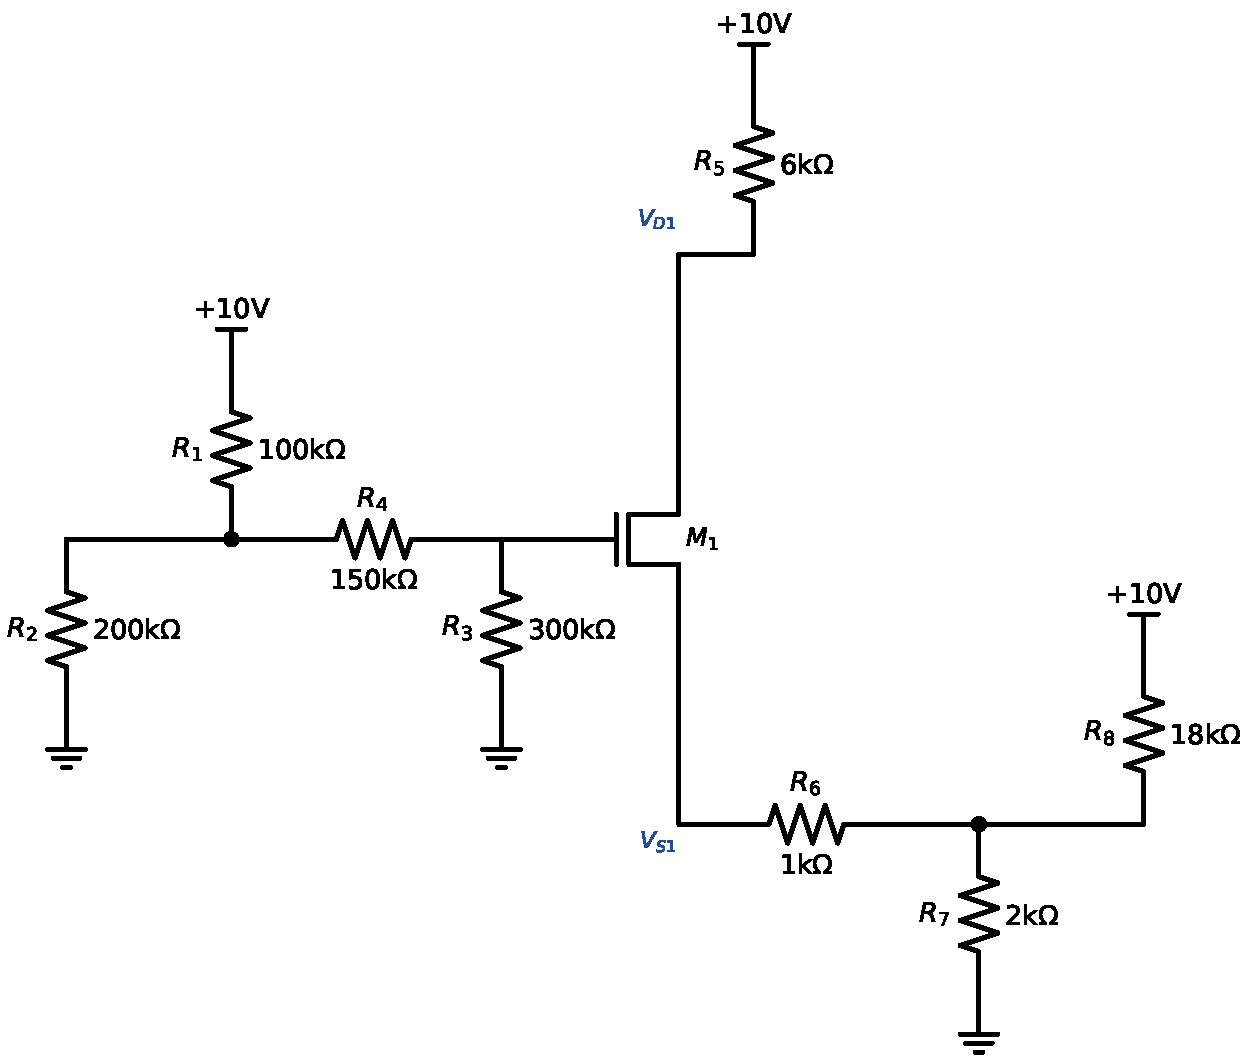
\includegraphics[width=0.9\linewidth,height=6cm,keepaspectratio]{p07_circuit}\end{center}
\solstep{1}{Why Thevenin}Plain KCL would need all 5 unknown node voltages at once, and the transistor equation is quadratic, so the elimination by hand is long. But each transistor touches every resistor network at a single terminal, and the gate draws no current. So every network can be replaced by its Thevenin pair $(V_{th}, R_{th})$ (tool T5), computed with the transistor removed --- 3 small networks, each a chain of dividers. What is left is one loop per transistor with a single quadratic.
\solstep{2}{Transistor $M_{1}$}\emph{Gate network} (seen from the gate of $M_{1}$, transistor removed). At $V_{x1}$ combine in parallel $R_{1}$ to $10$, $R_{2}$ to $0$ (Millman): \[V_{th} = \frac{\sum V_k/R_k}{\sum 1/R_k} = 6.667\,\mathrm{V},\qquad R_{th} = 100\,\mathrm{k}\Omega \| 200\,\mathrm{k}\Omega = 66.7\,\mathrm{k}\Omega\] Through $R_{4}$ in series: $R_{th}$ grows by $R_{4}$: $(V_{th}, R_{th}) = (6.667\,\mathrm{V},\ 217\,\mathrm{k}\Omega)$. At $V_{G1}$ combine in parallel the part already reduced, $R_{3}$ to $0$ (Millman): \[V_{th} = \frac{\sum V_k/R_k}{\sum 1/R_k} = 3.871\,\mathrm{V},\qquad R_{th} = 217\,\mathrm{k}\Omega \| 300\,\mathrm{k}\Omega = 126\,\mathrm{k}\Omega\] No current flows into the gate, so only $V_{th}$ matters: $V_{G1} = V_{th,G1} = 3.87\,\mathrm{V}$.

\emph{Source network} (seen from the source of $M_{1}$). At $V_{x2}$ combine in parallel $R_{7}$ to $0$, $R_{8}$ to $10$ (Millman): \[V_{th} = \frac{\sum V_k/R_k}{\sum 1/R_k} = 1\,\mathrm{V},\qquad R_{th} = 2\,\mathrm{k}\Omega \| 18\,\mathrm{k}\Omega = 1.8\,\mathrm{k}\Omega\] Through $R_{6}$ in series: $R_{th}$ grows by $R_{6}$: $(V_{th}, R_{th}) = (1\,\mathrm{V},\ 2.8\,\mathrm{k}\Omega)$.

\emph{Drain network} (seen from the drain of $M_{1}$). Start at $V_{D1}$: only $R_{5}$ to $10$, i.e. $(V_{th}, R_{th}) = (10\,\mathrm{V},\ 6\,\mathrm{k}\Omega)$.

With the networks replaced, $M_{1}$ sees one loop: gate at $3.87\,\mathrm{V}$, source through $R_{th,S1} = 2.8\,\mathrm{k}\Omega$ to $V_{th,S1} = 1\,\mathrm{V}$. KVL (assume $M_{1}$ active):\[V_{G1} - V_{th,S1} = 2.871 = V_{GS1} + R_{th,S1}I_{D1},\qquad I_{D1} = \frac{1.1\,\mathrm{m}}{2}(V_{GS1} - 1.4)^2\]\[1.54V_{GS1}^2 - 3.312V_{GS1} + 0.1474 = 0 \;\Rightarrow\; V_{GS1} = 0.04548\ \text{or}\ 2.105\,\mathrm{V}\]The root $0.0455$\,V is below $|V_t| = 1.4$\,V (the transistor would be off), so $V_{GS1} = 2.105$\,V. So $I_{D1} = 273\,\mu \mathrm{A}$.

Terminal voltages: $V_{S1} = V_{G1} - V_{GS1} = 1.77\,\mathrm{V}$, $V_{D1} = V_{th,D1} - R_{th,D1}I_{D1} = 10 - 6\,\mathrm{k}\times273\,\mu \mathrm{A} = 8.36\,\mathrm{V}$.

Check: $V_{DS1} = 6.593$\,V $\ge V_{ov1} = 0.705$\,V: $M_{1}$ is active \checkmark
\solstep{3}{Equivalent circuit}With every network replaced by its Thevenin pair the circuit is just this (the solution above is the analysis of this circuit):\begin{center}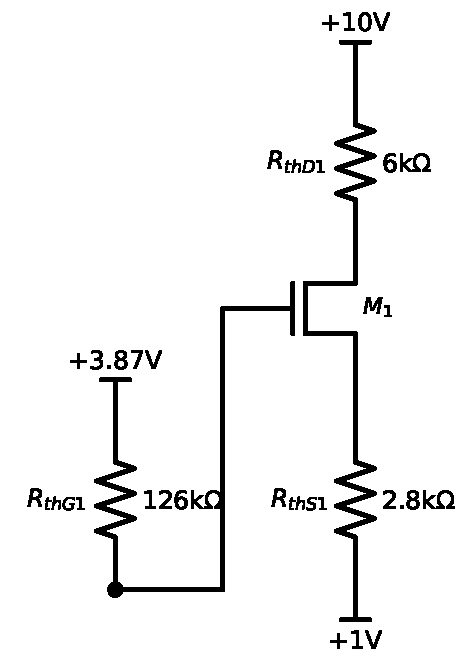
\includegraphics[width=0.6\linewidth,height=5cm,keepaspectratio]{p07_equivalent}\end{center}

A full nodal solve of the original circuit (all 5 node voltages) gives the same currents.
\begin{ansbox}
$I_{D1} = 273\,\mu \mathrm{A}$, $V_{S1} = 1.77\,\mathrm{V}$, $V_{D1} = 8.36\,\mathrm{V}$\\[2pt] all transistors active.
\end{ansbox}

\newpage
\subsection*{Solution 5F.8 \hfill Medium}
\begin{center}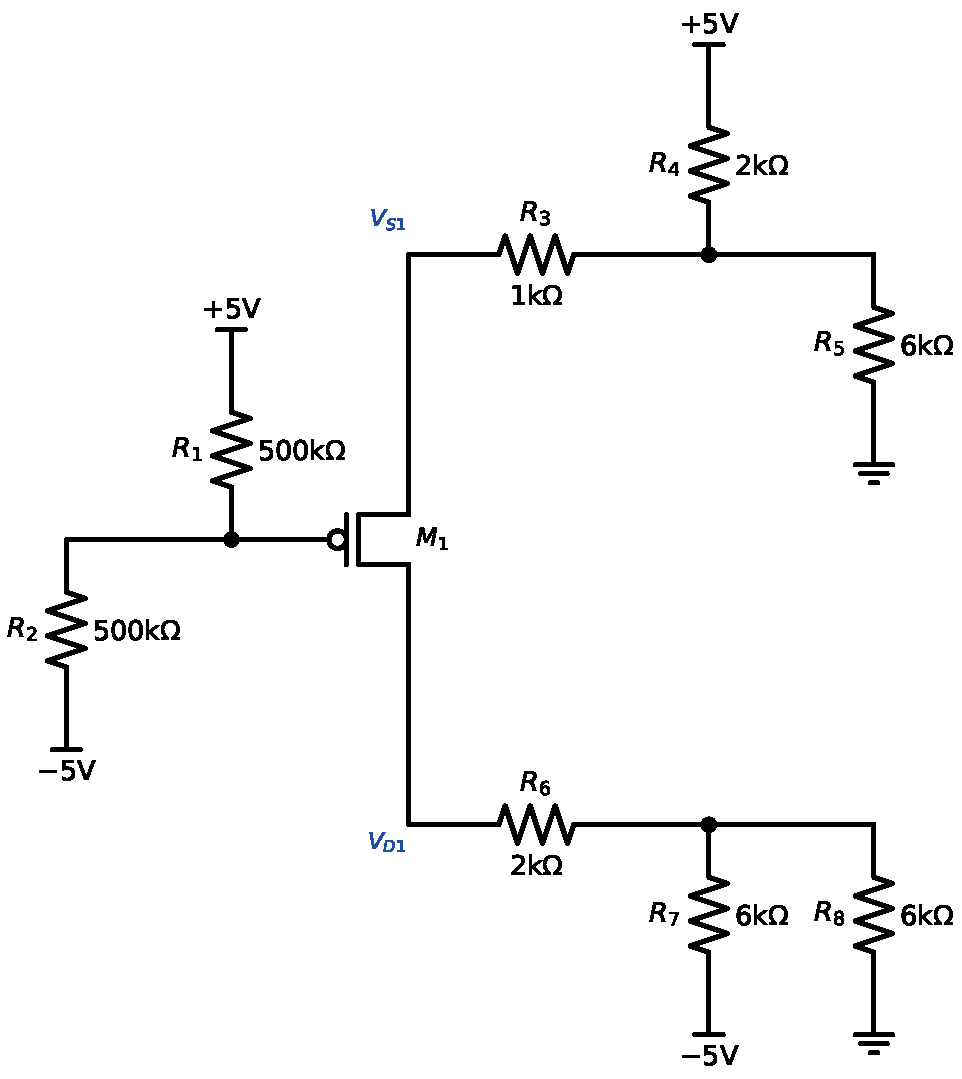
\includegraphics[width=0.9\linewidth,height=6cm,keepaspectratio]{p08_circuit}\end{center}
\solstep{1}{Why Thevenin}Plain KCL would need all 5 unknown node voltages at once, and the transistor equation is quadratic, so the elimination by hand is long. But each transistor touches every resistor network at a single terminal, and the gate draws no current. So every network can be replaced by its Thevenin pair $(V_{th}, R_{th})$ (tool T5), computed with the transistor removed --- 3 small networks, each a chain of dividers. What is left is one loop per transistor with a single quadratic.
\solstep{2}{Transistor $M_{1}$}\emph{Gate network} (seen from the gate of $M_{1}$, transistor removed). At $V_{G1}$ combine in parallel $R_{1}$ to $5$, $R_{2}$ to $(-5)$ (Millman): \[V_{th} = \frac{\sum V_k/R_k}{\sum 1/R_k} = 0\,\mathrm{V},\qquad R_{th} = 500\,\mathrm{k}\Omega \| 500\,\mathrm{k}\Omega = 250\,\mathrm{k}\Omega\] No current flows into the gate, so only $V_{th}$ matters: $V_{G1} = V_{th,G1} = 0\,\mathrm{V}$.

\emph{Source network} (seen from the source of $M_{1}$). At $V_{x1}$ combine in parallel $R_{4}$ to $5$, $R_{5}$ to $0$ (Millman): \[V_{th} = \frac{\sum V_k/R_k}{\sum 1/R_k} = 3.75\,\mathrm{V},\qquad R_{th} = 2\,\mathrm{k}\Omega \| 6\,\mathrm{k}\Omega = 1.5\,\mathrm{k}\Omega\] Through $R_{3}$ in series: $R_{th}$ grows by $R_{3}$: $(V_{th}, R_{th}) = (3.75\,\mathrm{V},\ 2.5\,\mathrm{k}\Omega)$.

\emph{Drain network} (seen from the drain of $M_{1}$). At $V_{x2}$ combine in parallel $R_{7}$ to $(-5)$, $R_{8}$ to $0$ (Millman): \[V_{th} = \frac{\sum V_k/R_k}{\sum 1/R_k} = -2.5\,\mathrm{V},\qquad R_{th} = 6\,\mathrm{k}\Omega \| 6\,\mathrm{k}\Omega = 3\,\mathrm{k}\Omega\] Through $R_{6}$ in series: $R_{th}$ grows by $R_{6}$: $(V_{th}, R_{th}) = (-2.5\,\mathrm{V},\ 5\,\mathrm{k}\Omega)$.

With the networks replaced, $M_{1}$ sees one loop: gate at $0\,\mathrm{V}$, source through $R_{th,S1} = 2.5\,\mathrm{k}\Omega$ to $V_{th,S1} = 3.75\,\mathrm{V}$. KVL (assume $M_{1}$ active):\[V_{th,S1} - V_{G1} = 3.75 = V_{SG1} + R_{th,S1}I_{D1},\qquad I_{D1} = \frac{850\,\mu }{2}(V_{SG1} - 1.3)^2\]\[1.062V_{SG1}^2 - 1.763V_{SG1} - 1.954 = 0 \;\Rightarrow\; V_{SG1} = -0.7603\ \text{or}\ 2.419\,\mathrm{V}\]The root $-0.76$\,V is below $|V_t| = 1.3$\,V (the transistor would be off), so $V_{SG1} = 2.419$\,V. So $I_{D1} = 532\,\mu \mathrm{A}$.

Terminal voltages: $V_{S1} = V_{G1} + V_{SG1} = 2.42\,\mathrm{V}$, $V_{D1} = V_{th,D1} + R_{th,D1}I_{D1} = -2.5 + 5\,\mathrm{k}\times532\,\mu \mathrm{A} = 0.162\,\mathrm{V}$.

Check: $V_{SD1} = 2.258$\,V $\ge V_{ov1} = 1.12$\,V: $M_{1}$ is active \checkmark
\solstep{3}{Equivalent circuit}With every network replaced by its Thevenin pair the circuit is just this (the solution above is the analysis of this circuit):\begin{center}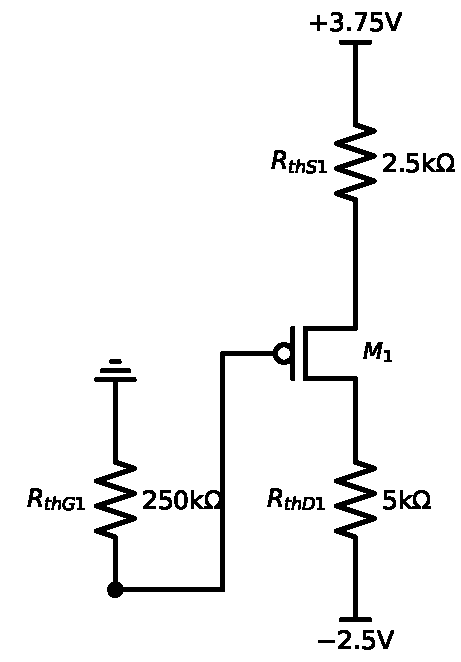
\includegraphics[width=0.6\linewidth,height=5cm,keepaspectratio]{p08_equivalent}\end{center}

A full nodal solve of the original circuit (all 5 node voltages) gives the same currents.
\begin{ansbox}
$I_{D1} = 532\,\mu \mathrm{A}$, $V_{S1} = 2.42\,\mathrm{V}$, $V_{D1} = 0.162\,\mathrm{V}$\\[2pt] all transistors active.
\end{ansbox}

\newpage
\subsection*{Solution 5F.9 \hfill Medium}
\begin{center}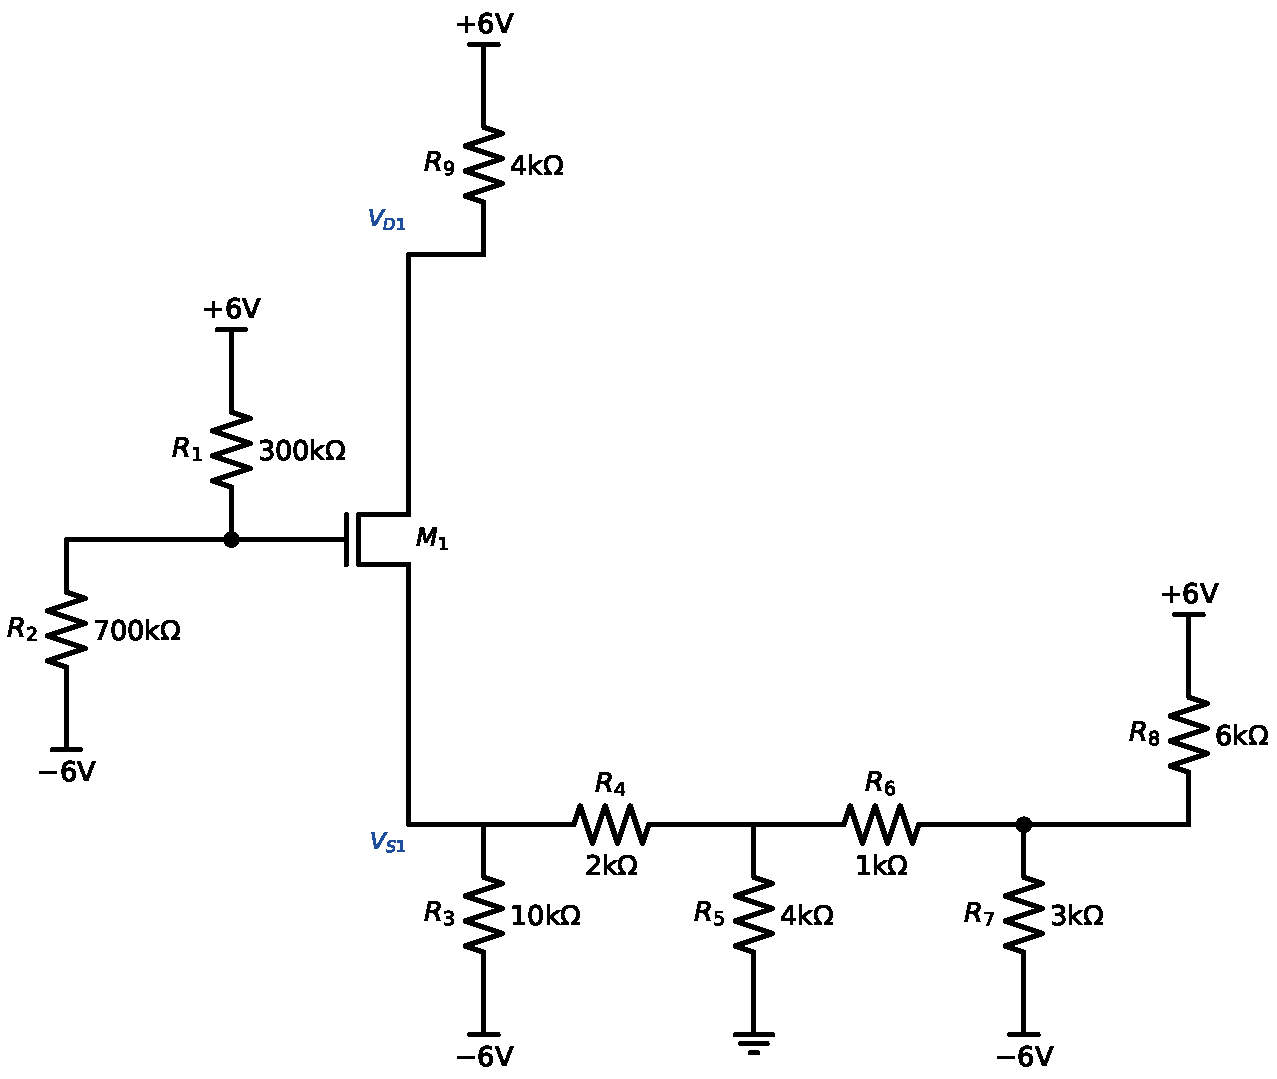
\includegraphics[width=0.9\linewidth,height=6cm,keepaspectratio]{p09_circuit}\end{center}
\solstep{1}{Why Thevenin}Plain KCL would need all 5 unknown node voltages at once, and the transistor equation is quadratic, so the elimination by hand is long. But each transistor touches every resistor network at a single terminal, and the gate draws no current. So every network can be replaced by its Thevenin pair $(V_{th}, R_{th})$ (tool T5), computed with the transistor removed --- 3 small networks, each a chain of dividers. What is left is one loop per transistor with a single quadratic.
\solstep{2}{Transistor $M_{1}$}\emph{Gate network} (seen from the gate of $M_{1}$, transistor removed). At $V_{G1}$ combine in parallel $R_{1}$ to $6$, $R_{2}$ to $(-6)$ (Millman): \[V_{th} = \frac{\sum V_k/R_k}{\sum 1/R_k} = 2.4\,\mathrm{V},\qquad R_{th} = 300\,\mathrm{k}\Omega \| 700\,\mathrm{k}\Omega = 210\,\mathrm{k}\Omega\] No current flows into the gate, so only $V_{th}$ matters: $V_{G1} = V_{th,G1} = 2.4\,\mathrm{V}$.

\emph{Source network} (seen from the source of $M_{1}$). At $V_{x2}$ combine in parallel $R_{7}$ to $(-6)$, $R_{8}$ to $6$ (Millman): \[V_{th} = \frac{\sum V_k/R_k}{\sum 1/R_k} = -2\,\mathrm{V},\qquad R_{th} = 3\,\mathrm{k}\Omega \| 6\,\mathrm{k}\Omega = 2\,\mathrm{k}\Omega\] Through $R_{6}$ in series: $R_{th}$ grows by $R_{6}$: $(V_{th}, R_{th}) = (-2\,\mathrm{V},\ 3\,\mathrm{k}\Omega)$. At $V_{x1}$ combine in parallel the part already reduced, $R_{5}$ to $0$ (Millman): \[V_{th} = \frac{\sum V_k/R_k}{\sum 1/R_k} = -1.143\,\mathrm{V},\qquad R_{th} = 3\,\mathrm{k}\Omega \| 4\,\mathrm{k}\Omega = 1.71\,\mathrm{k}\Omega\] Through $R_{4}$ in series: $R_{th}$ grows by $R_{4}$: $(V_{th}, R_{th}) = (-1.143\,\mathrm{V},\ 3.71\,\mathrm{k}\Omega)$. At $V_{S1}$ combine in parallel the part already reduced, $R_{3}$ to $(-6)$ (Millman): \[V_{th} = \frac{\sum V_k/R_k}{\sum 1/R_k} = -2.458\,\mathrm{V},\qquad R_{th} = 3.71\,\mathrm{k}\Omega \| 10\,\mathrm{k}\Omega = 2.71\,\mathrm{k}\Omega\]

\emph{Drain network} (seen from the drain of $M_{1}$). Start at $V_{D1}$: only $R_{9}$ to $6$, i.e. $(V_{th}, R_{th}) = (6\,\mathrm{V},\ 4\,\mathrm{k}\Omega)$.

With the networks replaced, $M_{1}$ sees one loop: gate at $2.4\,\mathrm{V}$, source through $R_{th,S1} = 2.71\,\mathrm{k}\Omega$ to $V_{th,S1} = -2.46\,\mathrm{V}$. KVL (assume $M_{1}$ active):\[V_{G1} - V_{th,S1} = 4.858 = V_{GS1} + R_{th,S1}I_{D1},\qquad I_{D1} = \frac{1.1\,\mathrm{m}}{2}(V_{GS1} - 1.4)^2\]\[1.49V_{GS1}^2 - 3.171V_{GS1} - 1.939 = 0 \;\Rightarrow\; V_{GS1} = -0.4959\ \text{or}\ 2.625\,\mathrm{V}\]The root $-0.496$\,V is below $|V_t| = 1.4$\,V (the transistor would be off), so $V_{GS1} = 2.625$\,V. So $I_{D1} = 825\,\mu \mathrm{A}$.

Terminal voltages: $V_{S1} = V_{G1} - V_{GS1} = -0.225\,\mathrm{V}$, $V_{D1} = V_{th,D1} - R_{th,D1}I_{D1} = 6 - 4\,\mathrm{k}\times825\,\mu \mathrm{A} = 2.7\,\mathrm{V}$.

Check: $V_{DS1} = 2.925$\,V $\ge V_{ov1} = 1.22$\,V: $M_{1}$ is active \checkmark
\solstep{3}{Equivalent circuit}With every network replaced by its Thevenin pair the circuit is just this (the solution above is the analysis of this circuit):\begin{center}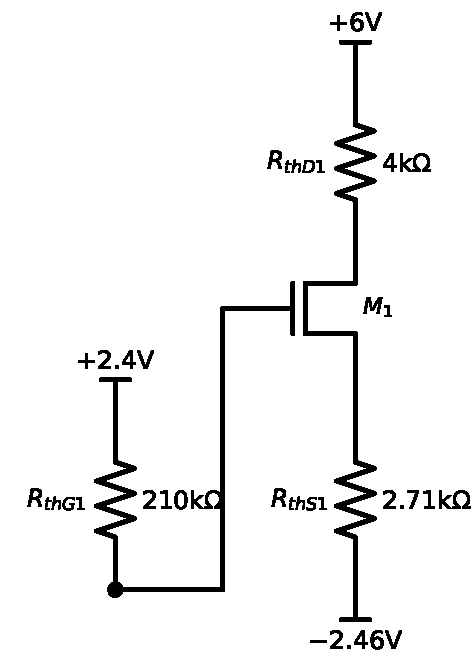
\includegraphics[width=0.6\linewidth,height=5cm,keepaspectratio]{p09_equivalent}\end{center}

A full nodal solve of the original circuit (all 5 node voltages) gives the same currents.
\begin{ansbox}
$I_{D1} = 825\,\mu \mathrm{A}$, $V_{S1} = -0.225\,\mathrm{V}$, $V_{D1} = 2.7\,\mathrm{V}$\\[2pt] all transistors active.
\end{ansbox}

\newpage
\subsection*{Solution 5F.10 \hfill Medium}
\begin{center}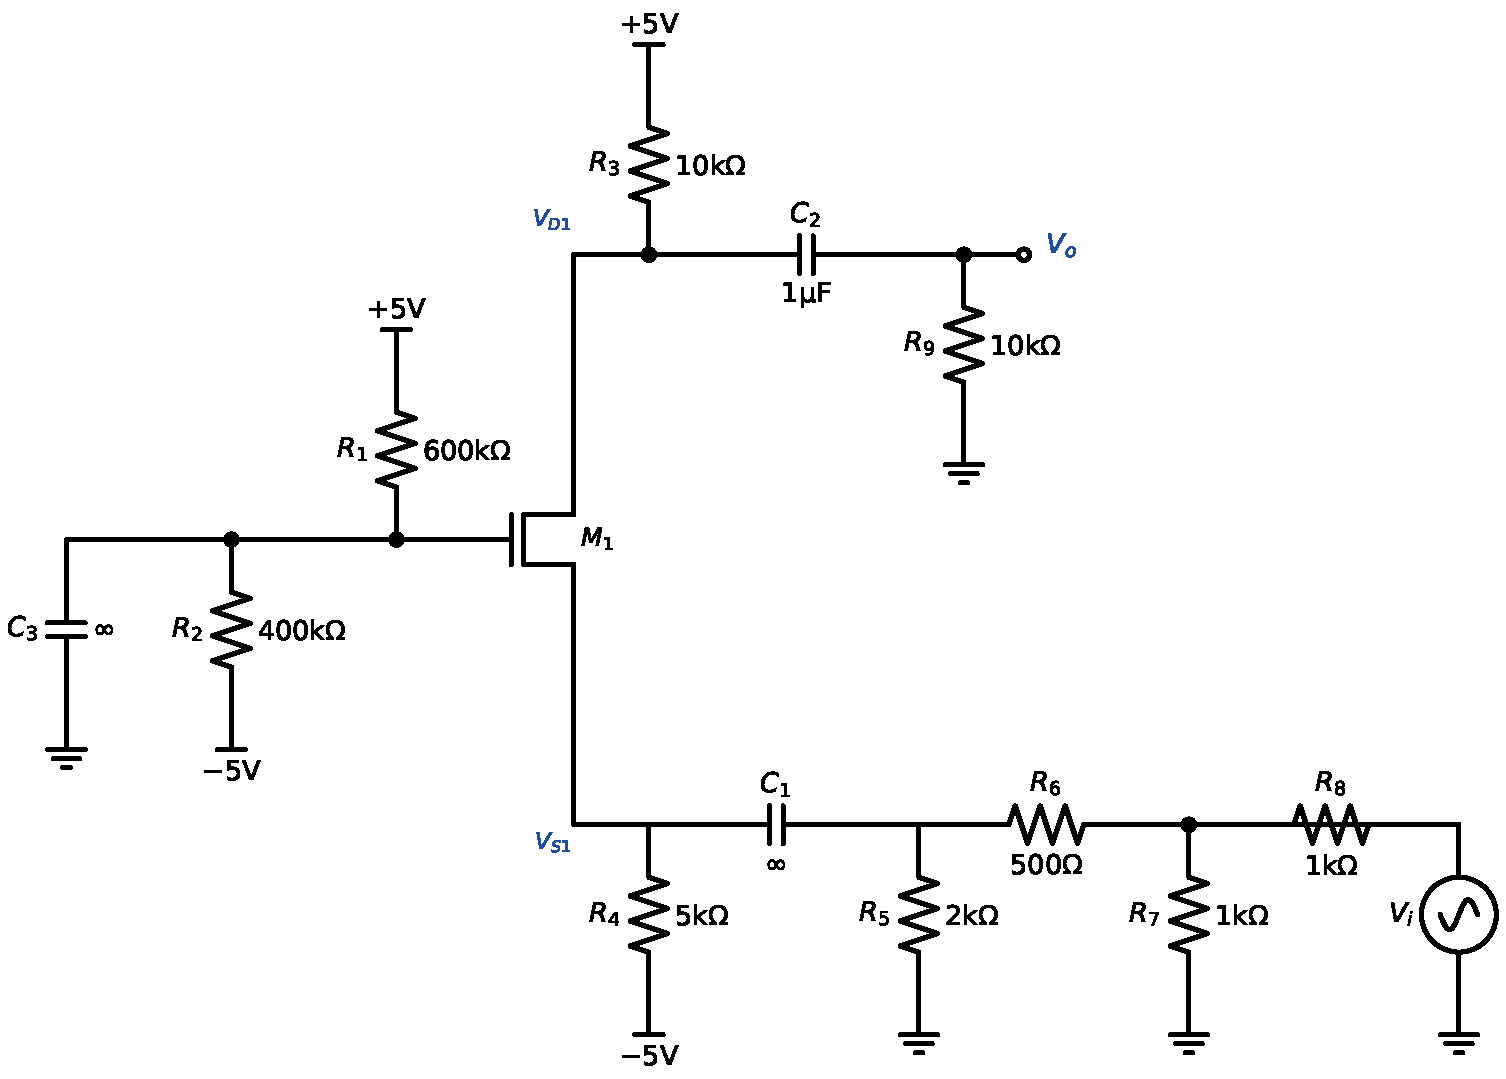
\includegraphics[width=0.9\linewidth,height=6cm,keepaspectratio]{p10_circuit}\end{center}
\solstep{1}{DC currents and transconductances}The DC drain currents are given: $I_{D1} = 359\,\mu \mathrm{A}$. For AC every supply is ground and every ``$\infty$'' capacitor is a short. Transconductances (tool T4):\begin{align*}
g_{m1} &= k_{1}V_{ov1} = \sqrt{2k_{1}I_{D1}} = \sqrt{2\cdot1.1\,\mathrm{m}\mathrm{A/V^2}\cdot359\,\mu \mathrm{A}} = 888\,\mu \mathrm{A/V},\qquad \frac{1}{g_{m1}} = 1.13\,\mathrm{k}\Omega\quad(V_{ov1} = 0.807\,\mathrm{V})
\end{align*}

\solstep{2}{Thevenin equivalent of the input network}Between $v_i$ and the source of $M_{1}$ there is a whole network (with KCL: one equation per node, in $s$). The transistor touches it only at its source, so replace it by its Thevenin pair $(V_{th}(s), Z_{th}(s))$ seen from there (tool T5), marching from the far end: At $V_{x2}$ combine in parallel $R_{7}$ to $0$, $R_{8}$ to $v_i$ (Millman): \[V_{th} = \frac{\sum V_k/Z_k}{\sum 1/Z_k} = 0.5\,v_i,\qquad Z_{th} = 1\,\mathrm{k}\Omega \| 1\,\mathrm{k}\Omega = 500\,\Omega\] Through $R_{6}$ in series: $Z_{th}$ grows by $R_{6}$: $(V_{th}, Z_{th}) = (0.5\,v_i,\ 1\,\mathrm{k}\Omega)$. At $V_{x1}$ combine in parallel the part already reduced, $R_{5}$ to $0$ (Millman): \[V_{th} = \frac{\sum V_k/Z_k}{\sum 1/Z_k} = 0.333\,v_i,\qquad Z_{th} = 1\,\mathrm{k}\Omega \| 2\,\mathrm{k}\Omega = 667\,\Omega\] $C_{1}$ is a short ($\infty$ capacitor): the pair is unchanged. At $V_{S1}$ combine in parallel the part already reduced, $R_{4}$ to $0$ (Millman): \[V_{th} = \frac{\sum V_k/Z_k}{\sum 1/Z_k} = 0.294\,v_i,\qquad Z_{th} = 667\,\Omega \| 5\,\mathrm{k}\Omega = 588\,\Omega\] The source of the common-gate stage presents $1/g_{m1} = 1.13\,\mathrm{k}\Omega$ to this Thevenin source, a voltage divider: \[\frac{v_{s1}}{v_i} = \frac{V_{th}}{v_i}\cdot\frac{1/g_{m1}}{Z_{th} + 1/g_{m1}} = 0.193\]
\solstep{3}{Rest of the signal path}Input resistance of every stage, from the last back to the first (each one loads the stage before it):\begin{align*}
R_{i1} &= Z_{source,1} = \frac{1}{g_{m1}} = 1.13\,\mathrm{k}\Omega\quad\text{(common gate)}
\end{align*}
Multiply the node-to-node gains along the signal path (tool T4):\[
H(s) = \frac{v_{d1}}{v_{s1}}\cdot\frac{v_o}{v_{d1}}
\]
\begin{align*}
\frac{v_{d1}}{v_{s1}} &= \frac{Z_{D1}}{1/g_{m1}},\quad Z_{D1} = R_{3} \parallel \left(\frac{1}{sC_{2}} + R_{9}\right)\ \Rightarrow\ \dfrac{4.44\,s + 444}{s + 50} \\
\frac{v_o}{v_{d1}} &= \frac{R_{9}}{\frac{1}{sC_{2}} + R_{9}} = \dfrac{s}{s + 100}
\end{align*}

\solstep{4}{Transfer function}Multiply and simplify:\[
H(s) = \dfrac{0.858\,s}{s + 50}
\]

\solstep{5}{Standard (Bode-ready) form}Find the roots. Every root $s=-p$ of the denominator is a \emph{pole}, every root $s=-z$ of the numerator is a \emph{zero}; $|p|$ and $|z|$ are the corner frequencies (rad/s).
\begin{itemize}[leftmargin=*,itemsep=2pt]
\item Numerator: it has the factor $s$ $\Rightarrow$ 1 zero at $s=0$.
\item Denominator: $s + 50$; $s + 50 = 0 \Rightarrow s = -50$.
\end{itemize}

Factored form (leading coefficient in front):
\[
H(s) = 0.858\,\dfrac{s}{(s+50)}
\]

Bode-ready form: rewrite every $(s+p) = p\left(1+\frac{s}{p}\right)$ and $(s+z) = z\left(1+\frac{s}{z}\right)$, and collect all constants into $K$. Each $s$ in the numerator is paired with one of the \emph{lowest} poles as $\frac{s}{s+p}$ (that factor is $\approx 1$ above $p$). Then every factor except $K$ is $\approx 1$ inside the pass-band:
\[
H(s) = 0.858\,\dfrac{s}{s+2\pi\cdot 7.96},\qquad K = 0.858
\]

\begin{center}\renewcommand{\arraystretch}{1.35}
\begin{tabular}{cccc}
\toprule
type & $\omega_c$ (rad/s) & $f_c=\omega_c/2\pi$ & slope change \\
\midrule
pole & $50$ & 7.96 Hz & $-20$ dB/dec \\
\bottomrule
\end{tabular}\end{center}

\solstep{6}{Magnitude Bode plot}Below every corner $|H(s)|\approx 0.0172\,s$, so the plot starts with a slope of $+20$\,dB/dec. Then, moving right, each pole bends the line down by 20\,dB/dec and each zero bends it up by 20\,dB/dec (tool T6):
\begin{center}\renewcommand{\arraystretch}{1.35}
\begin{tabular}{lcl}
\toprule
frequency range & slope & asymptote level \\
\midrule
$f<$ 7.96 Hz & $+20$ dB/dec & -1.33 dB at end \\
$f>$ 7.96 Hz & $0$ dB/dec (flat) & -1.33 dB at start \\
\bottomrule
\end{tabular}\end{center}

The flat (pass-band) level is $20\log_{10}|K| = 20\log_{10}0.858 = -1.33$\,dB.
\begin{center}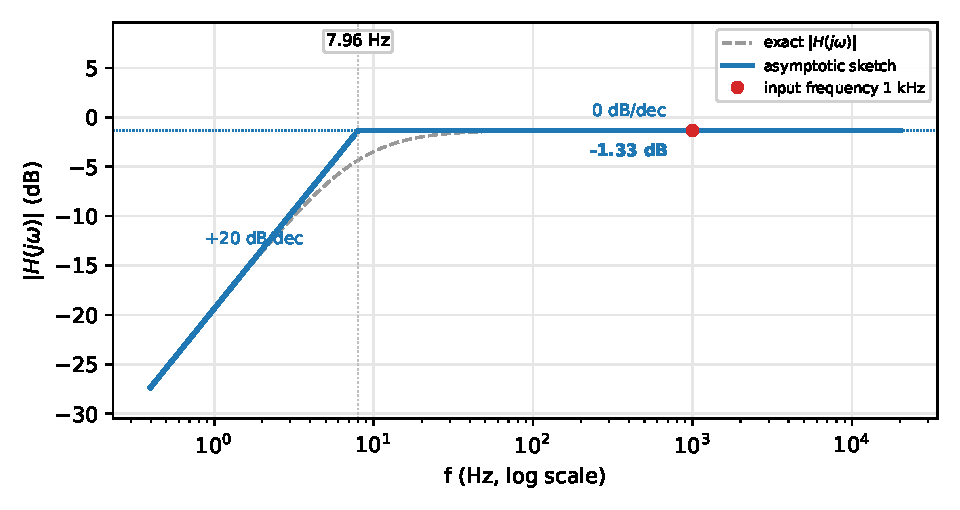
\includegraphics[width=0.78\linewidth,height=6.5cm,keepaspectratio]{p10_bode}\end{center}

{\small Blue: the straight-line sketch you are expected to draw. Dashed grey: the exact curve (about 3\,dB below the corner of an isolated pole). Red dot: the input frequency of Step 7.}
\solstep{7}{Steady-state output}The input is $V_i(t) = 0.01\sin\left(2\pi\cdot 1000\,t\right)$, so $\omega_{in} = 2\pi\cdot 1000 = 6280$\,rad/s. Put $s=j\omega_{in}$ in each factor (tool T5): magnitudes multiply, angles add.
{\small Rules: $\left|\frac{s}{s+p}\right| = \frac{\omega}{\sqrt{\omega^2+p^2}}$, $\angle = \frac{\pi}{2}-\tan^{-1}\frac{\omega}{p}$;\quad $\left|\frac{1}{1+s/p}\right| = \frac{1}{\sqrt{1+(\omega/p)^2}}$, $\angle = -\tan^{-1}\frac{\omega}{p}$;\quad $\left|1+\frac{s}{z}\right| = \sqrt{1+(\omega/z)^2}$, $\angle = \tan^{-1}\frac{\omega}{z}$;\quad a negative $K$ adds $-\pi$.}
\begin{center}\renewcommand{\arraystretch}{1.35}
\begin{tabular}{ccc}
\toprule
factor & magnitude & angle (rad) \\
\midrule
$0.858$ & $0.8579$ & $0$ \\
$\rule[-1.1em]{0pt}{2.8em}\dfrac{s}{s+2\pi\cdot 7.96}$ & $1$ & $0.00796$ \\
\textbf{total} & $\mathbf{0.8579}$ (product) & $\mathbf{0.00796}$ (sum) \\
\bottomrule
\end{tabular}\end{center}

\begin{align*}
|H(j\omega_{in})| &= 0.858, \qquad \angle H(j\omega_{in}) = 0.00796\ \mathrm{rad} \\
v_{o,ac}(t) &= 0.858\times 0.01\,\sin\left(2\pi\cdot 1000\,t + 0.00796\right) = 0.00858\,\sin\left(2\pi\cdot 1000\,t + 0.00796\right)
\end{align*}

\[
\boxed{V_o(t) = 0.00858\,\sin\left(2\pi\cdot 1000\,t + 0.00796\right)\ \mathrm{V}}
\]

\begin{ansbox}
$H(s) = 0.858\,\dfrac{s}{s+2\pi\cdot 7.96}$\quad (corners: 7.96 Hz)\\[4pt]
$V_o(t) = 0.00858\,\sin\left(2\pi\cdot 1000\,t + 0.00796\right)\ \mathrm{V}$
\end{ansbox}

\newpage
\subsection*{Solution 5F.11 \hfill Medium}
\begin{center}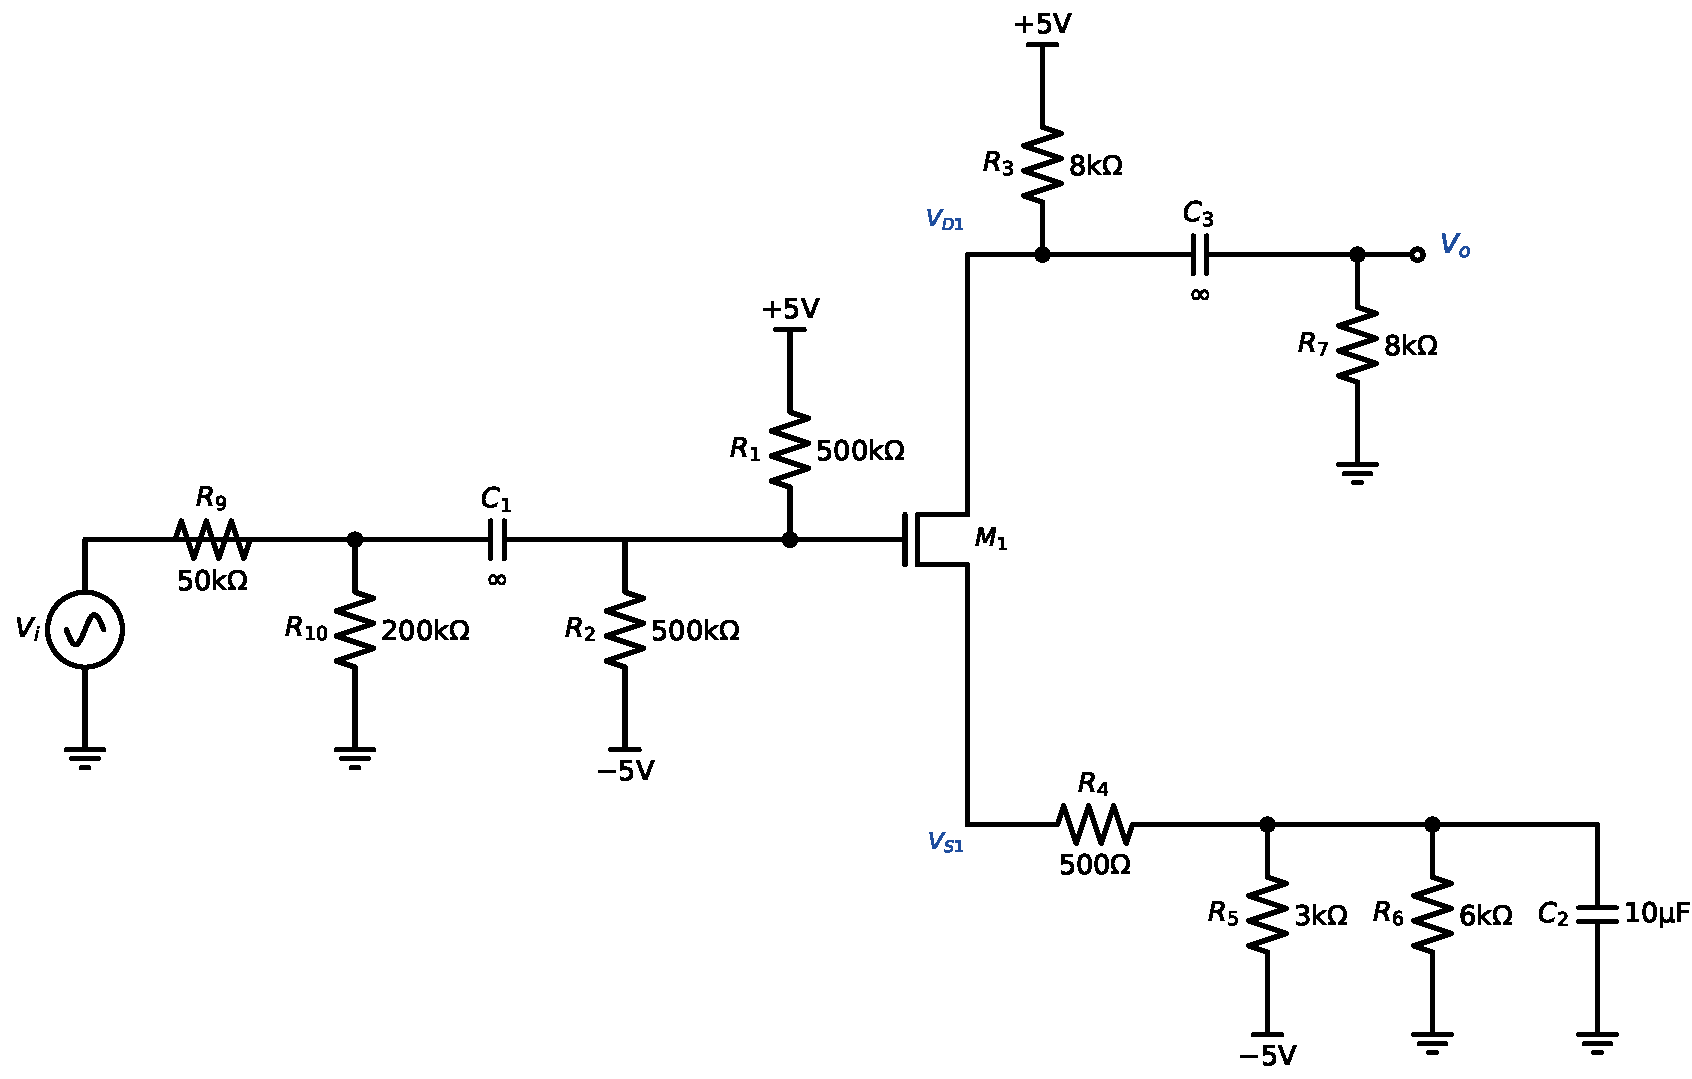
\includegraphics[width=0.9\linewidth,height=6cm,keepaspectratio]{p11_circuit}\end{center}
\solstep{1}{DC currents and transconductances}The DC drain currents are given: $I_{D1} = 423\,\mu \mathrm{A}$. For AC every supply is ground and every ``$\infty$'' capacitor is a short. Transconductances (tool T4):\begin{align*}
g_{m1} &= k_{1}V_{ov1} = \sqrt{2k_{1}I_{D1}} = \sqrt{2\cdot1.1\,\mathrm{m}\mathrm{A/V^2}\cdot423\,\mu \mathrm{A}} = 964\,\mu \mathrm{A/V},\qquad \frac{1}{g_{m1}} = 1.04\,\mathrm{k}\Omega\quad(V_{ov1} = 0.877\,\mathrm{V})
\end{align*}

\solstep{2}{Thevenin equivalent of the input network}Between $v_i$ and the gate of $M_{1}$ there is a whole network (with KCL: one equation per node, in $s$). The transistor touches it only at its gate, so replace it by its Thevenin pair $(V_{th}(s), Z_{th}(s))$ seen from there (tool T5), marching from the far end: At $V_{x0}$ combine in parallel $R_{9}$ to $v_i$, $R_{10}$ to $0$ (Millman): \[V_{th} = \frac{\sum V_k/Z_k}{\sum 1/Z_k} = 0.8\,v_i,\qquad Z_{th} = 50\,\mathrm{k}\Omega \| 200\,\mathrm{k}\Omega = 40\,\mathrm{k}\Omega\] $C_{1}$ is a short ($\infty$ capacitor): the pair is unchanged. At $V_{G1}$ combine in parallel the part already reduced, $R_{1}$ to $0$, $R_{2}$ to $0$ (Millman): \[V_{th} = \frac{\sum V_k/Z_k}{\sum 1/Z_k} = 0.69\,v_i,\qquad Z_{th} = 40\,\mathrm{k}\Omega \| 500\,\mathrm{k}\Omega \| 500\,\mathrm{k}\Omega = 34.5\,\mathrm{k}\Omega\] No current flows into the gate, so $Z_{th}$ plays no role: \[\frac{v_{g1}}{v_i} = \frac{V_{th}}{v_i} = 0.69\]
\solstep{3}{Rest of the signal path}Input resistance of every stage, from the last back to the first (each one loads the stage before it):\begin{align*}
R_{i1} &= Z_{gate,1} = \infty\quad\text{(input at the gate: it loads nothing)}
\end{align*}
Multiply the node-to-node gains along the signal path (tool T4):\[
H(s) = \frac{v_{d1}}{v_{g1}}
\]
\begin{align*}
\frac{v_{d1}}{v_{g1}} &= -\frac{Z_{D1}}{1/g_{m1} + Z_{S1}},\quad Z_{D1} = R_{3} \parallel R_{7},\ Z_{S1} = R_{4} + \left(R_{5} \parallel R_{6} \parallel \frac{1}{sC_{2}}\right)\ \Rightarrow\ \dfrac{-2.6\,s - 130}{s + 115}
\end{align*}

\solstep{4}{Transfer function}Multiply and simplify:\[
H(s) = \dfrac{-1.79\,s - 89.7}{s + 115}
\]

\solstep{5}{Standard (Bode-ready) form}Find the roots. Every root $s=-p$ of the denominator is a \emph{pole}, every root $s=-z$ of the numerator is a \emph{zero}; $|p|$ and $|z|$ are the corner frequencies (rad/s).
\begin{itemize}[leftmargin=*,itemsep=2pt]
\item Numerator: $-1.79\,s - 89.7$; divide by the leading coefficient $-1.79$ (this does not move the roots): $s + 50$; $s + 50 = 0 \Rightarrow s = -50$.
\item Denominator: $s + 115$; $s + 115 = 0 \Rightarrow s = -115$.
\end{itemize}

Factored form (leading coefficient in front):
\[
H(s) = -1.79\,\dfrac{(s+50)}{(s+115)}
\]

Bode-ready form: rewrite every $(s+p) = p\left(1+\frac{s}{p}\right)$ and $(s+z) = z\left(1+\frac{s}{z}\right)$, and collect all constants into $K$. Then every factor except $K$ is $\approx 1$ inside the pass-band:
\[
H(s) = -0.78\,\left(1+\dfrac{s}{2\pi\cdot 7.96}\right)\,\dfrac{1}{1+\dfrac{s}{2\pi\cdot 18.3}},\qquad K = -0.78
\]

\begin{center}\renewcommand{\arraystretch}{1.35}
\begin{tabular}{cccc}
\toprule
type & $\omega_c$ (rad/s) & $f_c=\omega_c/2\pi$ & slope change \\
\midrule
zero & $50$ & 7.96 Hz & $+20$ dB/dec \\
pole & $115$ & 18.3 Hz & $-20$ dB/dec \\
\bottomrule
\end{tabular}\end{center}

\solstep{6}{Magnitude Bode plot}Below every corner, all factors are $\approx$ constant: $|H| \approx 0.78$ $= -2.16$\,dB (flat, 0 dB/dec). Then, moving right, each pole bends the line down by 20\,dB/dec and each zero bends it up by 20\,dB/dec (tool T6):
\begin{center}\renewcommand{\arraystretch}{1.35}
\begin{tabular}{lcl}
\toprule
frequency range & slope & asymptote level \\
\midrule
$f<$ 7.96 Hz & $0$ dB/dec (flat) & -2.16 dB at end \\
7.96 Hz -- 18.3 Hz & $+20$ dB/dec & -2.16 dB at start, 5.08 dB at end \\
$f>$ 18.3 Hz & $0$ dB/dec (flat) & 5.08 dB at start \\
\bottomrule
\end{tabular}\end{center}

\begin{center}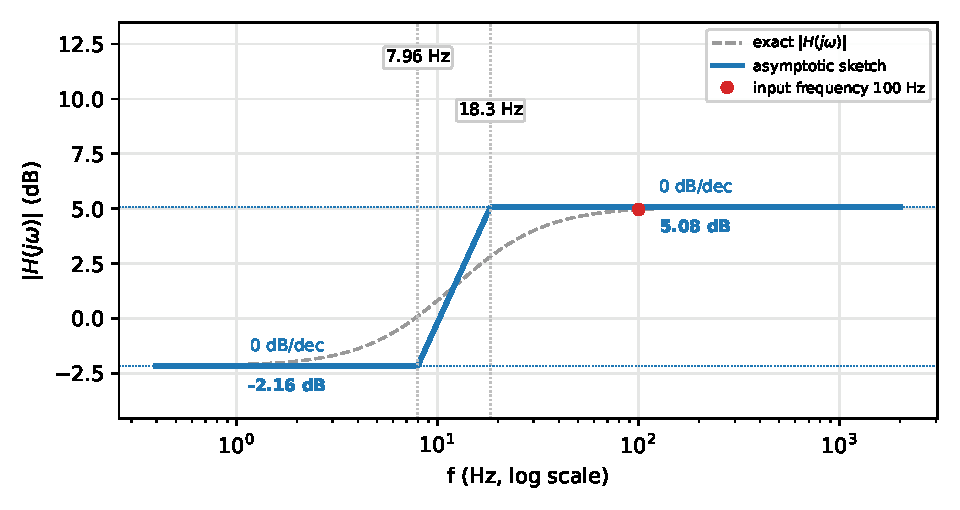
\includegraphics[width=0.78\linewidth,height=6.5cm,keepaspectratio]{p11_bode}\end{center}

{\small Blue: the straight-line sketch you are expected to draw. Dashed grey: the exact curve (about 3\,dB below the corner of an isolated pole). Red dot: the input frequency of Step 7.}
\solstep{7}{Steady-state output}The input is $V_i(t) = 0.01\sin\left(2\pi\cdot 100\,t\right)$, so $\omega_{in} = 2\pi\cdot 100 = 628$\,rad/s. Put $s=j\omega_{in}$ in each factor (tool T5): magnitudes multiply, angles add.
{\small Rules: $\left|\frac{s}{s+p}\right| = \frac{\omega}{\sqrt{\omega^2+p^2}}$, $\angle = \frac{\pi}{2}-\tan^{-1}\frac{\omega}{p}$;\quad $\left|\frac{1}{1+s/p}\right| = \frac{1}{\sqrt{1+(\omega/p)^2}}$, $\angle = -\tan^{-1}\frac{\omega}{p}$;\quad $\left|1+\frac{s}{z}\right| = \sqrt{1+(\omega/z)^2}$, $\angle = \tan^{-1}\frac{\omega}{z}$;\quad a negative $K$ adds $-\pi$.}
\begin{center}\renewcommand{\arraystretch}{1.35}
\begin{tabular}{ccc}
\toprule
factor & magnitude & angle (rad) \\
\midrule
$-0.78$ & $0.7799$ & $-3.14$ \\
$\rule[-1.1em]{0pt}{2.8em}\left(1+\dfrac{s}{2\pi\cdot 7.96}\right)$ & $12.61$ & $1.49$ \\
$\rule[-1.7em]{0pt}{4em}\dfrac{1}{1+\dfrac{s}{2\pi\cdot 18.3}}$ & $0.1801$ & $-1.39$ \\
\textbf{total} & $\mathbf{1.771}$ (product) & $\mathbf{-3.04}$ (sum) \\
\bottomrule
\end{tabular}\end{center}

\begin{align*}
|H(j\omega_{in})| &= 1.77, \qquad \angle H(j\omega_{in}) = -3.04\ \mathrm{rad} \\
v_{o,ac}(t) &= 1.77\times 0.01\,\sin\left(2\pi\cdot 100\,t - 3.04\right) = 0.0177\,\sin\left(2\pi\cdot 100\,t - 3.04\right)
\end{align*}

\[
\boxed{V_o(t) = 0.0177\,\sin\left(2\pi\cdot 100\,t - 3.04\right)\ \mathrm{V}}
\]

\begin{ansbox}
$H(s) = -0.78\,\left(1+\dfrac{s}{2\pi\cdot 7.96}\right)\,\dfrac{1}{1+\dfrac{s}{2\pi\cdot 18.3}}$\quad (corners: 7.96 Hz, 18.3 Hz)\\[4pt]
$V_o(t) = 0.0177\,\sin\left(2\pi\cdot 100\,t - 3.04\right)\ \mathrm{V}$
\end{ansbox}

\newpage
\subsection*{Solution 5F.12 \hfill Medium}
\begin{center}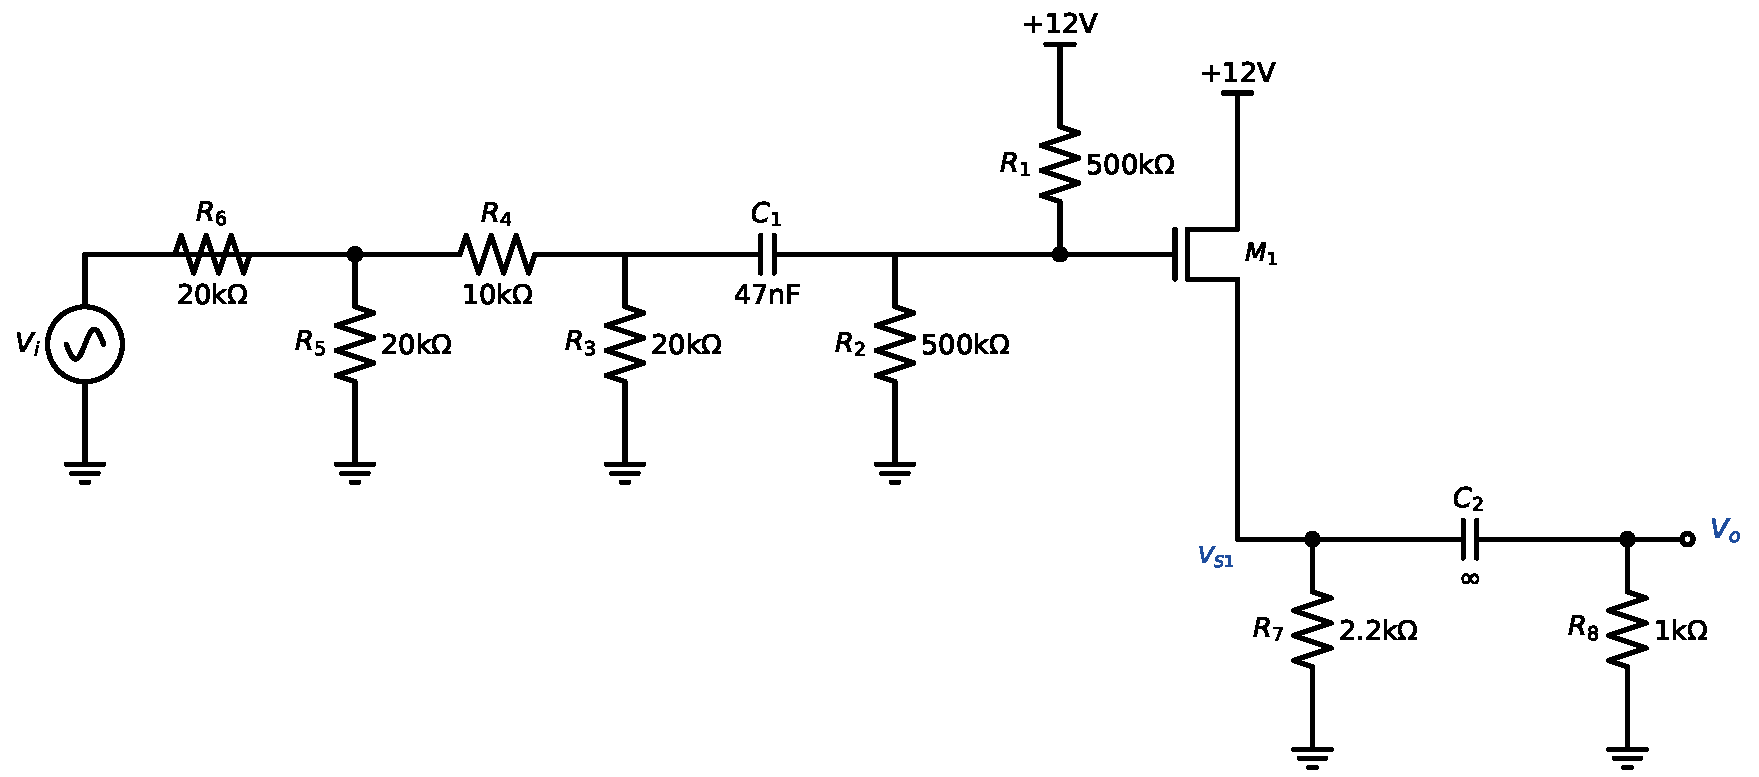
\includegraphics[width=0.9\linewidth,height=6cm,keepaspectratio]{p12_circuit}\end{center}
\solstep{1}{DC currents and transconductances}The DC drain currents are given: $I_{D1} = 1.37\,\mathrm{m}\mathrm{A}$. For AC every supply is ground and every ``$\infty$'' capacitor is a short. Transconductances (tool T4):\begin{align*}
g_{m1} &= k_{1}V_{ov1} = \sqrt{2k_{1}I_{D1}} = \sqrt{2\cdot1.1\,\mathrm{m}\mathrm{A/V^2}\cdot1.37\,\mathrm{m}\mathrm{A}} = 1.74\,\mathrm{m}\mathrm{A/V},\qquad \frac{1}{g_{m1}} = 575\,\Omega\quad(V_{ov1} = 1.58\,\mathrm{V})
\end{align*}

\solstep{2}{Thevenin equivalent of the input network}Between $v_i$ and the gate of $M_{1}$ there is a whole network (with KCL: one equation per node, in $s$). The transistor touches it only at its gate, so replace it by its Thevenin pair $(V_{th}(s), Z_{th}(s))$ seen from there (tool T5), marching from the far end: At $V_{x2}$ combine in parallel $R_{5}$ to $0$, $R_{6}$ to $v_i$ (Millman): \[V_{th} = \frac{\sum V_k/Z_k}{\sum 1/Z_k} = 0.5\,v_i,\qquad Z_{th} = 20\,\mathrm{k}\Omega \| 20\,\mathrm{k}\Omega = 10\,\mathrm{k}\Omega\] Through $R_{4}$ in series: $Z_{th}$ grows by $R_{4}$: $(V_{th}, Z_{th}) = (0.5\,v_i,\ 20\,\mathrm{k}\Omega)$. At $V_{x1}$ combine in parallel the part already reduced, $R_{3}$ to $0$ (Millman): \[V_{th} = \frac{\sum V_k/Z_k}{\sum 1/Z_k} = 0.25\,v_i,\qquad Z_{th} = 20\,\mathrm{k}\Omega \| 20\,\mathrm{k}\Omega = 10\,\mathrm{k}\Omega\] Through $C_{1}$ in series: $Z_{th}$ grows by $\frac{1}{sC_{1}}$: $(V_{th}, Z_{th}) = (0.25\,v_i,\ \dfrac{10000\,s + 2.13\times 10^{7}}{s})$. At $V_{G1}$ combine in parallel the part already reduced, $R_{1}$ to $0$, $R_{2}$ to $0$ (Millman): \[V_{th} = \frac{\sum V_k/Z_k}{\sum 1/Z_k} = \dfrac{0.24\,s}{s + 81.8}\,v_i,\qquad Z_{th} = \dfrac{10000\,s + 2.13\times 10^{7}}{s} \| 500\,\mathrm{k}\Omega \| 500\,\mathrm{k}\Omega = \dfrac{9620\,s + 2.05\times 10^{7}}{s + 81.8}\] No current flows into the gate, so $Z_{th}$ plays no role: \[\frac{v_{g1}}{v_i} = \frac{V_{th}}{v_i} = \dfrac{0.24\,s}{s + 81.8}\]
\solstep{3}{Rest of the signal path}Input resistance of every stage, from the last back to the first (each one loads the stage before it):\begin{align*}
R_{i1} &= Z_{gate,1} = \infty\quad\text{(input at the gate: it loads nothing)}
\end{align*}
Multiply the node-to-node gains along the signal path (tool T4):\[
H(s) = \frac{v_{s1}}{v_{g1}}
\]
\begin{align*}
\frac{v_{s1}}{v_{g1}} &= \frac{Z_{S1}}{1/g_{m1} + Z_{S1}},\quad Z_{S1} = R_{7} \parallel R_{8}\ \Rightarrow\ 0.544
\end{align*}

\solstep{4}{Transfer function}Multiply and simplify:\[
H(s) = \dfrac{0.131\,s}{s + 81.8}
\]

\solstep{5}{Standard (Bode-ready) form}Find the roots. Every root $s=-p$ of the denominator is a \emph{pole}, every root $s=-z$ of the numerator is a \emph{zero}; $|p|$ and $|z|$ are the corner frequencies (rad/s).
\begin{itemize}[leftmargin=*,itemsep=2pt]
\item Numerator: it has the factor $s$ $\Rightarrow$ 1 zero at $s=0$.
\item Denominator: $s + 81.8$; $s + 81.8 = 0 \Rightarrow s = -81.8$.
\end{itemize}

Factored form (leading coefficient in front):
\[
H(s) = 0.131\,\dfrac{s}{(s+81.8)}
\]

Bode-ready form: rewrite every $(s+p) = p\left(1+\frac{s}{p}\right)$ and $(s+z) = z\left(1+\frac{s}{z}\right)$, and collect all constants into $K$. Each $s$ in the numerator is paired with one of the \emph{lowest} poles as $\frac{s}{s+p}$ (that factor is $\approx 1$ above $p$). Then every factor except $K$ is $\approx 1$ inside the pass-band:
\[
H(s) = 0.131\,\dfrac{s}{s+2\pi\cdot 13},\qquad K = 0.131
\]

\begin{center}\renewcommand{\arraystretch}{1.35}
\begin{tabular}{cccc}
\toprule
type & $\omega_c$ (rad/s) & $f_c=\omega_c/2\pi$ & slope change \\
\midrule
pole & $81.8$ & 13 Hz & $-20$ dB/dec \\
\bottomrule
\end{tabular}\end{center}

\solstep{6}{Magnitude Bode plot}Below every corner $|H(s)|\approx 0.0016\,s$, so the plot starts with a slope of $+20$\,dB/dec. Then, moving right, each pole bends the line down by 20\,dB/dec and each zero bends it up by 20\,dB/dec (tool T6):
\begin{center}\renewcommand{\arraystretch}{1.35}
\begin{tabular}{lcl}
\toprule
frequency range & slope & asymptote level \\
\midrule
$f<$ 13 Hz & $+20$ dB/dec & -17.7 dB at end \\
$f>$ 13 Hz & $0$ dB/dec (flat) & -17.7 dB at start \\
\bottomrule
\end{tabular}\end{center}

The flat (pass-band) level is $20\log_{10}|K| = 20\log_{10}0.131 = -17.7$\,dB.
\begin{center}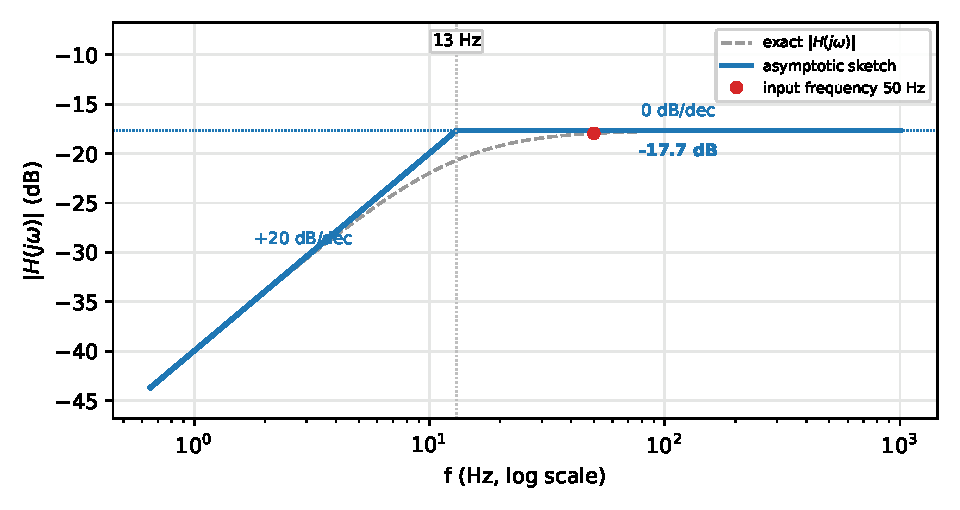
\includegraphics[width=0.78\linewidth,height=6.5cm,keepaspectratio]{p12_bode}\end{center}

{\small Blue: the straight-line sketch you are expected to draw. Dashed grey: the exact curve (about 3\,dB below the corner of an isolated pole). Red dot: the input frequency of Step 7.}
\solstep{7}{Steady-state output}The input is $V_i(t) = 0.5\sin\left(2\pi\cdot 50\,t\right)$, so $\omega_{in} = 2\pi\cdot 50 = 314$\,rad/s. Put $s=j\omega_{in}$ in each factor (tool T5): magnitudes multiply, angles add.
{\small Rules: $\left|\frac{s}{s+p}\right| = \frac{\omega}{\sqrt{\omega^2+p^2}}$, $\angle = \frac{\pi}{2}-\tan^{-1}\frac{\omega}{p}$;\quad $\left|\frac{1}{1+s/p}\right| = \frac{1}{\sqrt{1+(\omega/p)^2}}$, $\angle = -\tan^{-1}\frac{\omega}{p}$;\quad $\left|1+\frac{s}{z}\right| = \sqrt{1+(\omega/z)^2}$, $\angle = \tan^{-1}\frac{\omega}{z}$;\quad a negative $K$ adds $-\pi$.}
\begin{center}\renewcommand{\arraystretch}{1.35}
\begin{tabular}{ccc}
\toprule
factor & magnitude & angle (rad) \\
\midrule
$0.131$ & $0.1309$ & $0$ \\
$\rule[-1.1em]{0pt}{2.8em}\dfrac{s}{s+2\pi\cdot 13}$ & $0.9677$ & $0.255$ \\
\textbf{total} & $\mathbf{0.1266}$ (product) & $\mathbf{0.255}$ (sum) \\
\bottomrule
\end{tabular}\end{center}

\begin{align*}
|H(j\omega_{in})| &= 0.127, \qquad \angle H(j\omega_{in}) = 0.255\ \mathrm{rad} \\
v_{o,ac}(t) &= 0.127\times 0.5\,\sin\left(2\pi\cdot 50\,t + 0.255\right) = 0.0633\,\sin\left(2\pi\cdot 50\,t + 0.255\right)
\end{align*}

\[
\boxed{V_o(t) = 0.0633\,\sin\left(2\pi\cdot 50\,t + 0.255\right)\ \mathrm{V}}
\]

\begin{ansbox}
$H(s) = 0.131\,\dfrac{s}{s+2\pi\cdot 13}$\quad (corners: 13 Hz)\\[4pt]
$V_o(t) = 0.0633\,\sin\left(2\pi\cdot 50\,t + 0.255\right)\ \mathrm{V}$
\end{ansbox}

\newpage
\subsection*{Solution 5F.13 \hfill Hard}
\begin{center}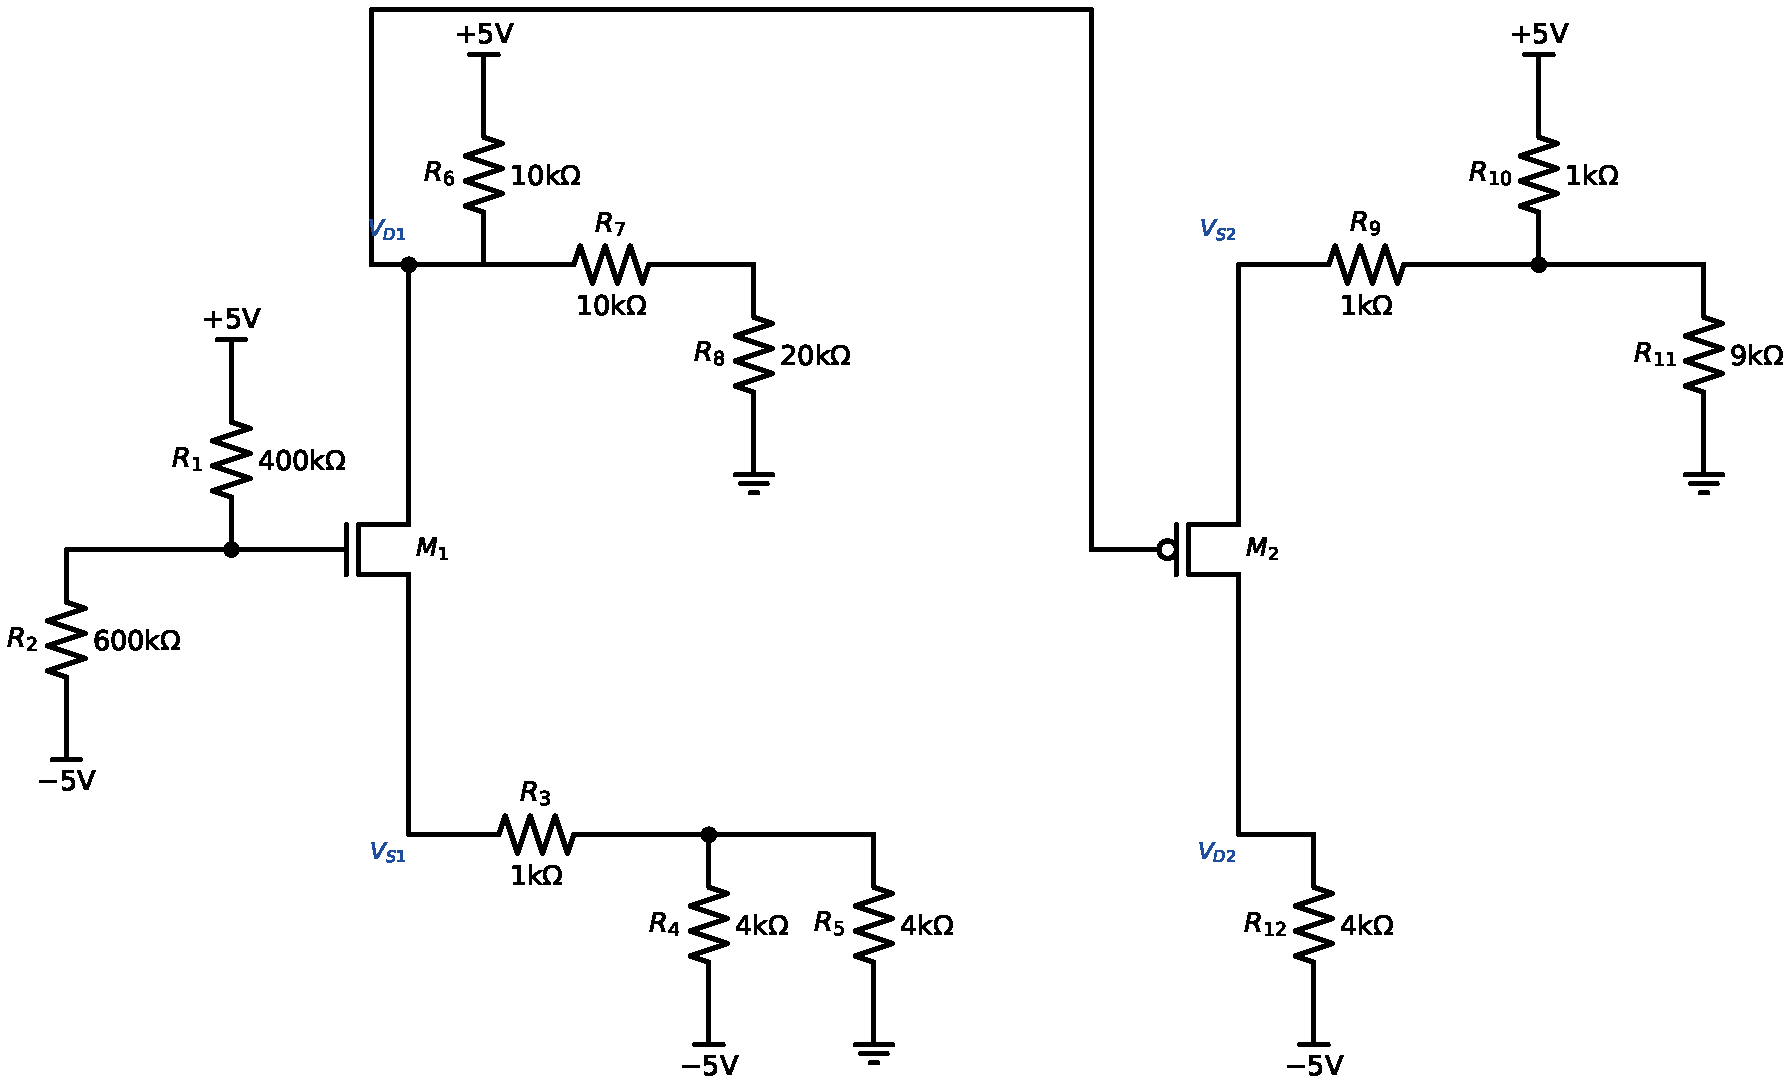
\includegraphics[width=0.9\linewidth,height=6cm,keepaspectratio]{p13_circuit}\end{center}
\solstep{1}{Why Thevenin}Plain KCL would need all 8 unknown node voltages at once, and the transistor equation is quadratic, so the elimination by hand is long. But each transistor touches every resistor network at a single terminal, and the gate draws no current. So every network can be replaced by its Thevenin pair $(V_{th}, R_{th})$ (tool T5), computed with the transistor removed --- 5 small networks, each a chain of dividers. What is left is one loop per transistor with a single quadratic.
\solstep{2}{Transistor $M_{1}$}\emph{Gate network} (seen from the gate of $M_{1}$, transistor removed). At $V_{G1}$ combine in parallel $R_{1}$ to $5$, $R_{2}$ to $(-5)$ (Millman): \[V_{th} = \frac{\sum V_k/R_k}{\sum 1/R_k} = 1\,\mathrm{V},\qquad R_{th} = 400\,\mathrm{k}\Omega \| 600\,\mathrm{k}\Omega = 240\,\mathrm{k}\Omega\] No current flows into the gate, so only $V_{th}$ matters: $V_{G1} = V_{th,G1} = 1\,\mathrm{V}$.

\emph{Source network} (seen from the source of $M_{1}$). At $V_{x1}$ combine in parallel $R_{4}$ to $(-5)$, $R_{5}$ to $0$ (Millman): \[V_{th} = \frac{\sum V_k/R_k}{\sum 1/R_k} = -2.5\,\mathrm{V},\qquad R_{th} = 4\,\mathrm{k}\Omega \| 4\,\mathrm{k}\Omega = 2\,\mathrm{k}\Omega\] Through $R_{3}$ in series: $R_{th}$ grows by $R_{3}$: $(V_{th}, R_{th}) = (-2.5\,\mathrm{V},\ 3\,\mathrm{k}\Omega)$.

\emph{Drain network} (seen from the drain of $M_{1}$). Start at $V_{x2}$: only $R_{8}$ to $0$, i.e. $(V_{th}, R_{th}) = (0\,\mathrm{V},\ 20\,\mathrm{k}\Omega)$. Through $R_{7}$ in series: $R_{th}$ grows by $R_{7}$: $(V_{th}, R_{th}) = (0\,\mathrm{V},\ 30\,\mathrm{k}\Omega)$. At $V_{D1}$ combine in parallel the part already reduced, $R_{6}$ to $5$ (Millman): \[V_{th} = \frac{\sum V_k/R_k}{\sum 1/R_k} = 3.75\,\mathrm{V},\qquad R_{th} = 30\,\mathrm{k}\Omega \| 10\,\mathrm{k}\Omega = 7.5\,\mathrm{k}\Omega\]

With the networks replaced, $M_{1}$ sees one loop: gate at $1\,\mathrm{V}$, source through $R_{th,S1} = 3\,\mathrm{k}\Omega$ to $V_{th,S1} = -2.5\,\mathrm{V}$. KVL (assume $M_{1}$ active):\[V_{G1} - V_{th,S1} = 3.5 = V_{GS1} + R_{th,S1}I_{D1},\qquad I_{D1} = \frac{1.1\,\mathrm{m}}{2}(V_{GS1} - 1.4)^2\]\[1.65V_{GS1}^2 - 3.62V_{GS1} - 0.266 = 0 \;\Rightarrow\; V_{GS1} = -0.07117\ \text{or}\ 2.265\,\mathrm{V}\]The root $-0.0712$\,V is below $|V_t| = 1.4$\,V (the transistor would be off), so $V_{GS1} = 2.265$\,V. So $I_{D1} = 412\,\mu \mathrm{A}$.

Terminal voltages: $V_{S1} = V_{G1} - V_{GS1} = -1.27\,\mathrm{V}$, $V_{D1} = V_{th,D1} - R_{th,D1}I_{D1} = 3.75 - 7.5\,\mathrm{k}\times412\,\mu \mathrm{A} = 0.663\,\mathrm{V}$.

Check: $V_{DS1} = 1.928$\,V $\ge V_{ov1} = 0.865$\,V: $M_{1}$ is active \checkmark
\solstep{3}{Transistor $M_{2}$}The gate of $M_{2}$ is node $V_{D1}$, already known: $V_{D1} = 0.663\,\mathrm{V}$.

\emph{Source network} (seen from the source of $M_{2}$). At $V_{x3}$ combine in parallel $R_{10}$ to $5$, $R_{11}$ to $0$ (Millman): \[V_{th} = \frac{\sum V_k/R_k}{\sum 1/R_k} = 4.5\,\mathrm{V},\qquad R_{th} = 1\,\mathrm{k}\Omega \| 9\,\mathrm{k}\Omega = 900\,\Omega\] Through $R_{9}$ in series: $R_{th}$ grows by $R_{9}$: $(V_{th}, R_{th}) = (4.5\,\mathrm{V},\ 1.9\,\mathrm{k}\Omega)$.

\emph{Drain network} (seen from the drain of $M_{2}$). Start at $V_{D2}$: only $R_{12}$ to $(-5)$, i.e. $(V_{th}, R_{th}) = (-5\,\mathrm{V},\ 4\,\mathrm{k}\Omega)$.

With the networks replaced, $M_{2}$ sees one loop: gate at $0.663\,\mathrm{V}$, source through $R_{th,S2} = 1.9\,\mathrm{k}\Omega$ to $V_{th,S2} = 4.5\,\mathrm{V}$. KVL (assume $M_{2}$ active):\[V_{th,S2} - V_{G2} = 3.837 = V_{SG2} + R_{th,S2}I_{D2},\qquad I_{D2} = \frac{850\,\mu }{2}(V_{SG2} - 1.3)^2\]\[0.8075V_{SG2}^2 - 1.099V_{SG2} - 2.473 = 0 \;\Rightarrow\; V_{SG2} = -1.197\ \text{or}\ 2.558\,\mathrm{V}\]The root $-1.2$\,V is below $|V_t| = 1.3$\,V (the transistor would be off), so $V_{SG2} = 2.558$\,V. So $I_{D2} = 673\,\mu \mathrm{A}$.

Terminal voltages: $V_{S2} = V_{D1} + V_{SG2} = 3.22\,\mathrm{V}$, $V_{D2} = V_{th,D2} + R_{th,D2}I_{D2} = -5 + 4\,\mathrm{k}\times673\,\mu \mathrm{A} = -2.31\,\mathrm{V}$.

Check: $V_{SD2} = 5.529$\,V $\ge V_{ov2} = 1.26$\,V: $M_{2}$ is active \checkmark
\solstep{4}{Equivalent circuit}With every network replaced by its Thevenin pair the circuit is just this (the solution above is the analysis of this circuit):\begin{center}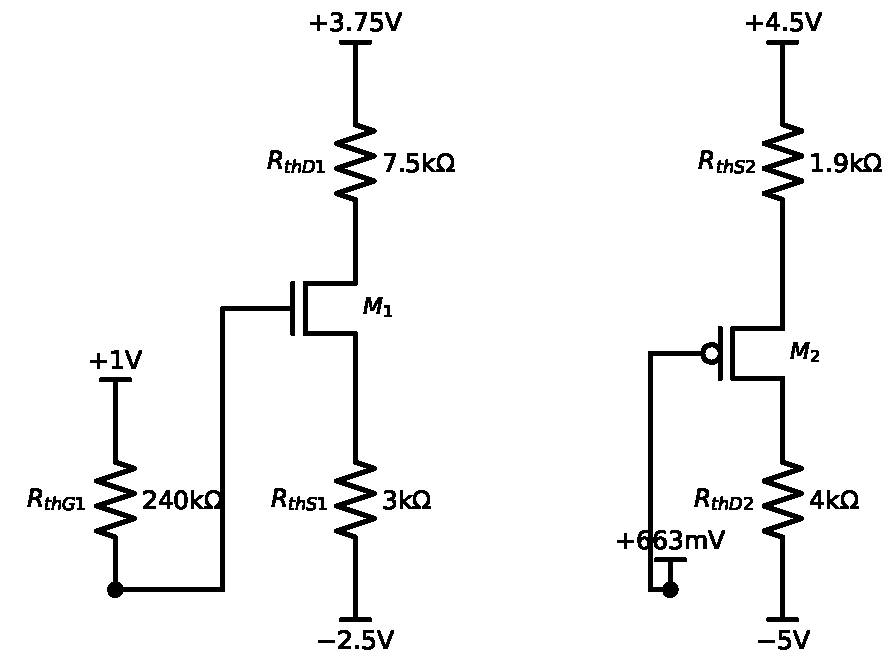
\includegraphics[width=0.6\linewidth,height=5cm,keepaspectratio]{p13_equivalent}\end{center}

A full nodal solve of the original circuit (all 8 node voltages) gives the same currents.
\begin{ansbox}
$I_{D1} = 412\,\mu \mathrm{A}$, $V_{S1} = -1.27\,\mathrm{V}$, $V_{D1} = 0.663\,\mathrm{V}$,\quad $I_{D2} = 673\,\mu \mathrm{A}$, $V_{S2} = 3.22\,\mathrm{V}$, $V_{D2} = -2.31\,\mathrm{V}$\\[2pt] all transistors active.
\end{ansbox}

\newpage
\subsection*{Solution 5F.14 \hfill Hard}
\begin{center}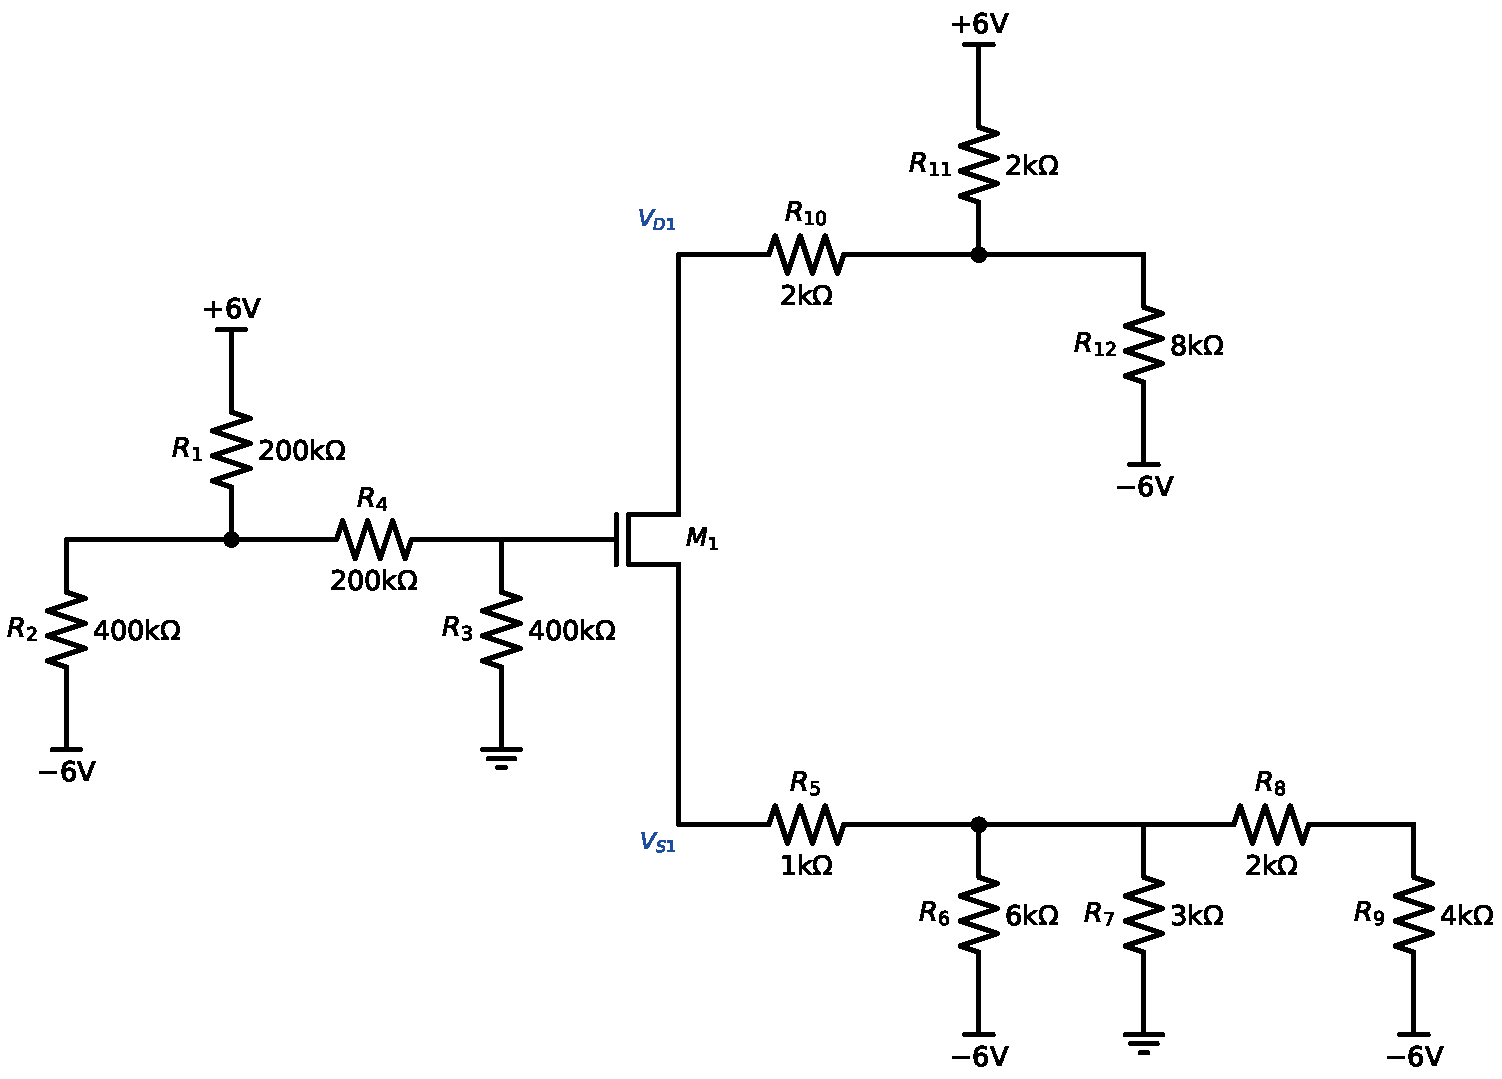
\includegraphics[width=0.9\linewidth,height=6cm,keepaspectratio]{p14_circuit}\end{center}
\solstep{1}{Why Thevenin}Plain KCL would need all 7 unknown node voltages at once, and the transistor equation is quadratic, so the elimination by hand is long. But each transistor touches every resistor network at a single terminal, and the gate draws no current. So every network can be replaced by its Thevenin pair $(V_{th}, R_{th})$ (tool T5), computed with the transistor removed --- 3 small networks, each a chain of dividers. What is left is one loop per transistor with a single quadratic.
\solstep{2}{Transistor $M_{1}$}\emph{Gate network} (seen from the gate of $M_{1}$, transistor removed). At $V_{x1}$ combine in parallel $R_{1}$ to $6$, $R_{2}$ to $(-6)$ (Millman): \[V_{th} = \frac{\sum V_k/R_k}{\sum 1/R_k} = 2\,\mathrm{V},\qquad R_{th} = 200\,\mathrm{k}\Omega \| 400\,\mathrm{k}\Omega = 133\,\mathrm{k}\Omega\] Through $R_{4}$ in series: $R_{th}$ grows by $R_{4}$: $(V_{th}, R_{th}) = (2\,\mathrm{V},\ 333\,\mathrm{k}\Omega)$. At $V_{G1}$ combine in parallel the part already reduced, $R_{3}$ to $0$ (Millman): \[V_{th} = \frac{\sum V_k/R_k}{\sum 1/R_k} = 1.091\,\mathrm{V},\qquad R_{th} = 333\,\mathrm{k}\Omega \| 400\,\mathrm{k}\Omega = 182\,\mathrm{k}\Omega\] No current flows into the gate, so only $V_{th}$ matters: $V_{G1} = V_{th,G1} = 1.09\,\mathrm{V}$.

\emph{Source network} (seen from the source of $M_{1}$). Start at $V_{x3}$: only $R_{9}$ to $(-6)$, i.e. $(V_{th}, R_{th}) = (-6\,\mathrm{V},\ 4\,\mathrm{k}\Omega)$. Through $R_{8}$ in series: $R_{th}$ grows by $R_{8}$: $(V_{th}, R_{th}) = (-6\,\mathrm{V},\ 6\,\mathrm{k}\Omega)$. At $V_{x2}$ combine in parallel the part already reduced, $R_{6}$ to $(-6)$, $R_{7}$ to $0$ (Millman): \[V_{th} = \frac{\sum V_k/R_k}{\sum 1/R_k} = -3\,\mathrm{V},\qquad R_{th} = 6\,\mathrm{k}\Omega \| 6\,\mathrm{k}\Omega \| 3\,\mathrm{k}\Omega = 1.5\,\mathrm{k}\Omega\] Through $R_{5}$ in series: $R_{th}$ grows by $R_{5}$: $(V_{th}, R_{th}) = (-3\,\mathrm{V},\ 2.5\,\mathrm{k}\Omega)$.

\emph{Drain network} (seen from the drain of $M_{1}$). At $V_{x4}$ combine in parallel $R_{11}$ to $6$, $R_{12}$ to $(-6)$ (Millman): \[V_{th} = \frac{\sum V_k/R_k}{\sum 1/R_k} = 3.6\,\mathrm{V},\qquad R_{th} = 2\,\mathrm{k}\Omega \| 8\,\mathrm{k}\Omega = 1.6\,\mathrm{k}\Omega\] Through $R_{10}$ in series: $R_{th}$ grows by $R_{10}$: $(V_{th}, R_{th}) = (3.6\,\mathrm{V},\ 3.6\,\mathrm{k}\Omega)$.

With the networks replaced, $M_{1}$ sees one loop: gate at $1.09\,\mathrm{V}$, source through $R_{th,S1} = 2.5\,\mathrm{k}\Omega$ to $V_{th,S1} = -3\,\mathrm{V}$. KVL (assume $M_{1}$ active):\[V_{G1} - V_{th,S1} = 4.091 = V_{GS1} + R_{th,S1}I_{D1},\qquad I_{D1} = \frac{1.1\,\mathrm{m}}{2}(V_{GS1} - 1.4)^2\]\[1.375V_{GS1}^2 - 2.85V_{GS1} - 1.396 = 0 \;\Rightarrow\; V_{GS1} = -0.4091\ \text{or}\ 2.482\,\mathrm{V}\]The root $-0.409$\,V is below $|V_t| = 1.4$\,V (the transistor would be off), so $V_{GS1} = 2.482$\,V. So $I_{D1} = 644\,\mu \mathrm{A}$.

Terminal voltages: $V_{S1} = V_{G1} - V_{GS1} = -1.39\,\mathrm{V}$, $V_{D1} = V_{th,D1} - R_{th,D1}I_{D1} = 3.6 - 3.6\,\mathrm{k}\times644\,\mu \mathrm{A} = 1.28\,\mathrm{V}$.

Check: $V_{DS1} = 2.674$\,V $\ge V_{ov1} = 1.08$\,V: $M_{1}$ is active \checkmark
\solstep{3}{Equivalent circuit}With every network replaced by its Thevenin pair the circuit is just this (the solution above is the analysis of this circuit):\begin{center}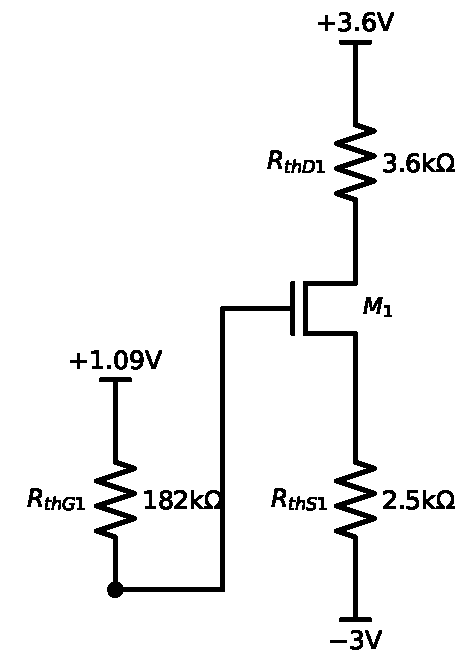
\includegraphics[width=0.6\linewidth,height=5cm,keepaspectratio]{p14_equivalent}\end{center}

A full nodal solve of the original circuit (all 7 node voltages) gives the same currents.
\begin{ansbox}
$I_{D1} = 644\,\mu \mathrm{A}$, $V_{S1} = -1.39\,\mathrm{V}$, $V_{D1} = 1.28\,\mathrm{V}$\\[2pt] all transistors active.
\end{ansbox}

\newpage
\subsection*{Solution 5F.15 \hfill Hard}
\begin{center}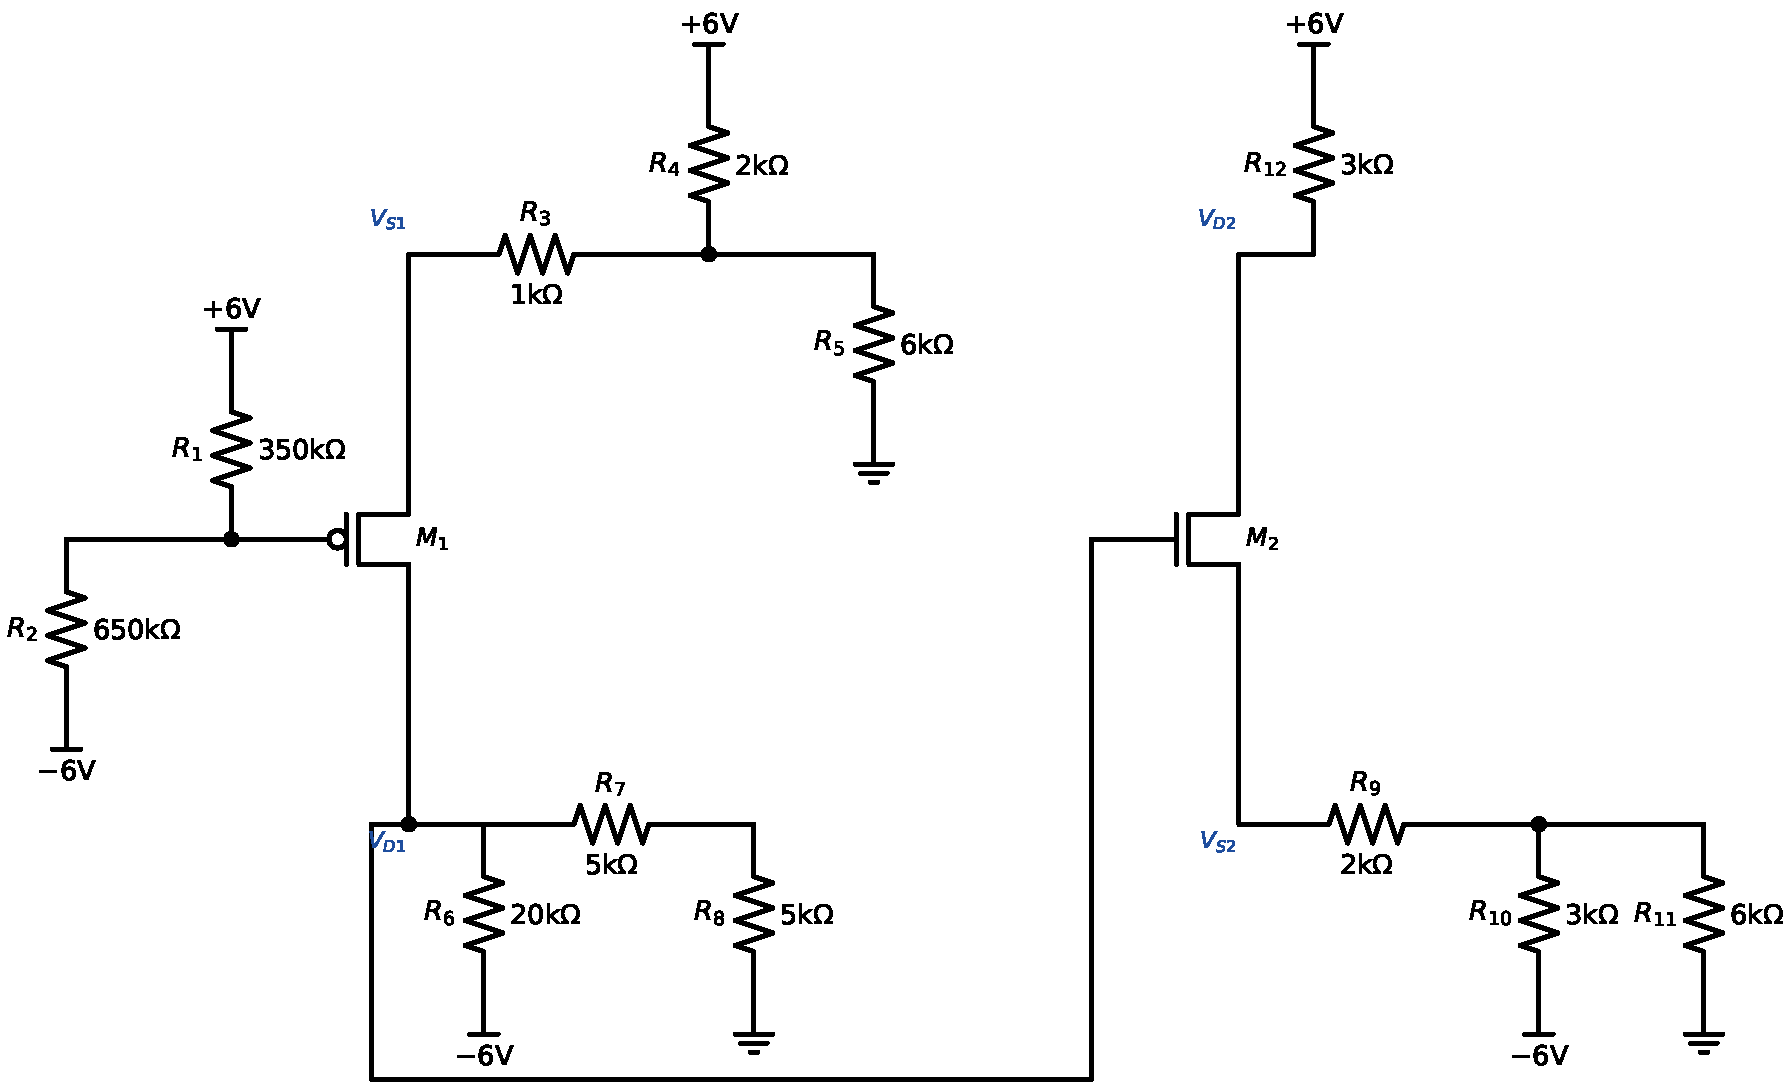
\includegraphics[width=0.9\linewidth,height=6cm,keepaspectratio]{p15_circuit}\end{center}
\solstep{1}{Why Thevenin}Plain KCL would need all 8 unknown node voltages at once, and the transistor equation is quadratic, so the elimination by hand is long. But each transistor touches every resistor network at a single terminal, and the gate draws no current. So every network can be replaced by its Thevenin pair $(V_{th}, R_{th})$ (tool T5), computed with the transistor removed --- 5 small networks, each a chain of dividers. What is left is one loop per transistor with a single quadratic.
\solstep{2}{Transistor $M_{1}$}\emph{Gate network} (seen from the gate of $M_{1}$, transistor removed). At $V_{G1}$ combine in parallel $R_{1}$ to $6$, $R_{2}$ to $(-6)$ (Millman): \[V_{th} = \frac{\sum V_k/R_k}{\sum 1/R_k} = 1.8\,\mathrm{V},\qquad R_{th} = 350\,\mathrm{k}\Omega \| 650\,\mathrm{k}\Omega = 227\,\mathrm{k}\Omega\] No current flows into the gate, so only $V_{th}$ matters: $V_{G1} = V_{th,G1} = 1.8\,\mathrm{V}$.

\emph{Source network} (seen from the source of $M_{1}$). At $V_{x1}$ combine in parallel $R_{4}$ to $6$, $R_{5}$ to $0$ (Millman): \[V_{th} = \frac{\sum V_k/R_k}{\sum 1/R_k} = 4.5\,\mathrm{V},\qquad R_{th} = 2\,\mathrm{k}\Omega \| 6\,\mathrm{k}\Omega = 1.5\,\mathrm{k}\Omega\] Through $R_{3}$ in series: $R_{th}$ grows by $R_{3}$: $(V_{th}, R_{th}) = (4.5\,\mathrm{V},\ 2.5\,\mathrm{k}\Omega)$.

\emph{Drain network} (seen from the drain of $M_{1}$). Start at $V_{x2}$: only $R_{8}$ to $0$, i.e. $(V_{th}, R_{th}) = (0\,\mathrm{V},\ 5\,\mathrm{k}\Omega)$. Through $R_{7}$ in series: $R_{th}$ grows by $R_{7}$: $(V_{th}, R_{th}) = (0\,\mathrm{V},\ 10\,\mathrm{k}\Omega)$. At $V_{D1}$ combine in parallel the part already reduced, $R_{6}$ to $(-6)$ (Millman): \[V_{th} = \frac{\sum V_k/R_k}{\sum 1/R_k} = -2\,\mathrm{V},\qquad R_{th} = 10\,\mathrm{k}\Omega \| 20\,\mathrm{k}\Omega = 6.67\,\mathrm{k}\Omega\]

With the networks replaced, $M_{1}$ sees one loop: gate at $1.8\,\mathrm{V}$, source through $R_{th,S1} = 2.5\,\mathrm{k}\Omega$ to $V_{th,S1} = 4.5\,\mathrm{V}$. KVL (assume $M_{1}$ active):\[V_{th,S1} - V_{G1} = 2.7 = V_{SG1} + R_{th,S1}I_{D1},\qquad I_{D1} = \frac{850\,\mu }{2}(V_{SG1} - 1.3)^2\]\[1.062V_{SG1}^2 - 1.763V_{SG1} - 0.9044 = 0 \;\Rightarrow\; V_{SG1} = -0.4112\ \text{or}\ 2.07\,\mathrm{V}\]The root $-0.411$\,V is below $|V_t| = 1.3$\,V (the transistor would be off), so $V_{SG1} = 2.07$\,V. So $I_{D1} = 252\,\mu \mathrm{A}$.

Terminal voltages: $V_{S1} = V_{G1} + V_{SG1} = 3.87\,\mathrm{V}$, $V_{D1} = V_{th,D1} + R_{th,D1}I_{D1} = -2 + 6.67\,\mathrm{k}\times252\,\mu \mathrm{A} = -0.32\,\mathrm{V}$.

Check: $V_{SD1} = 4.19$\,V $\ge V_{ov1} = 0.77$\,V: $M_{1}$ is active \checkmark
\solstep{3}{Transistor $M_{2}$}The gate of $M_{2}$ is node $V_{D1}$, already known: $V_{D1} = -0.32\,\mathrm{V}$.

\emph{Source network} (seen from the source of $M_{2}$). At $V_{x3}$ combine in parallel $R_{10}$ to $(-6)$, $R_{11}$ to $0$ (Millman): \[V_{th} = \frac{\sum V_k/R_k}{\sum 1/R_k} = -4\,\mathrm{V},\qquad R_{th} = 3\,\mathrm{k}\Omega \| 6\,\mathrm{k}\Omega = 2\,\mathrm{k}\Omega\] Through $R_{9}$ in series: $R_{th}$ grows by $R_{9}$: $(V_{th}, R_{th}) = (-4\,\mathrm{V},\ 4\,\mathrm{k}\Omega)$.

\emph{Drain network} (seen from the drain of $M_{2}$). Start at $V_{D2}$: only $R_{12}$ to $6$, i.e. $(V_{th}, R_{th}) = (6\,\mathrm{V},\ 3\,\mathrm{k}\Omega)$.

With the networks replaced, $M_{2}$ sees one loop: gate at $-0.32\,\mathrm{V}$, source through $R_{th,S2} = 4\,\mathrm{k}\Omega$ to $V_{th,S2} = -4\,\mathrm{V}$. KVL (assume $M_{2}$ active):\[V_{G2} - V_{th,S2} = 3.68 = V_{GS2} + R_{th,S2}I_{D2},\qquad I_{D2} = \frac{1.1\,\mathrm{m}}{2}(V_{GS2} - 1.4)^2\]\[2.2V_{GS2}^2 - 5.16V_{GS2} + 0.632 = 0 \;\Rightarrow\; V_{GS2} = 0.1297\ \text{or}\ 2.216\,\mathrm{V}\]The root $0.13$\,V is below $|V_t| = 1.4$\,V (the transistor would be off), so $V_{GS2} = 2.216$\,V. So $I_{D2} = 366\,\mu \mathrm{A}$.

Terminal voltages: $V_{S2} = V_{D1} - V_{GS2} = -2.54\,\mathrm{V}$, $V_{D2} = V_{th,D2} - R_{th,D2}I_{D2} = 6 - 3\,\mathrm{k}\times366\,\mu \mathrm{A} = 4.9\,\mathrm{V}$.

Check: $V_{DS2} = 7.438$\,V $\ge V_{ov2} = 0.816$\,V: $M_{2}$ is active \checkmark
\solstep{4}{Equivalent circuit}With every network replaced by its Thevenin pair the circuit is just this (the solution above is the analysis of this circuit):\begin{center}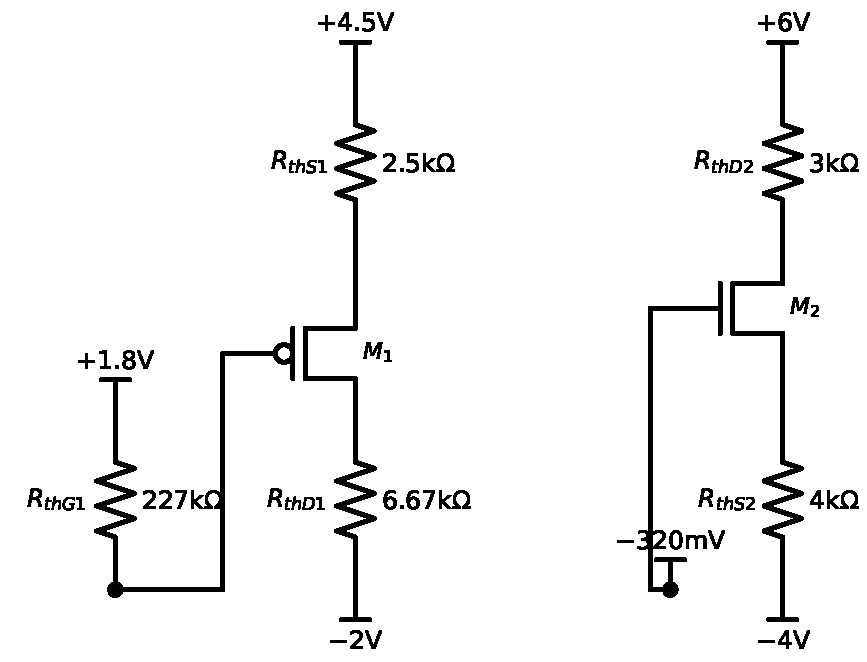
\includegraphics[width=0.6\linewidth,height=5cm,keepaspectratio]{p15_equivalent}\end{center}

A full nodal solve of the original circuit (all 8 node voltages) gives the same currents.
\begin{ansbox}
$I_{D1} = 252\,\mu \mathrm{A}$, $V_{S1} = 3.87\,\mathrm{V}$, $V_{D1} = -0.32\,\mathrm{V}$,\quad $I_{D2} = 366\,\mu \mathrm{A}$, $V_{S2} = -2.54\,\mathrm{V}$, $V_{D2} = 4.9\,\mathrm{V}$\\[2pt] all transistors active.
\end{ansbox}

\newpage
\subsection*{Solution 5F.16 \hfill Hard}
\begin{center}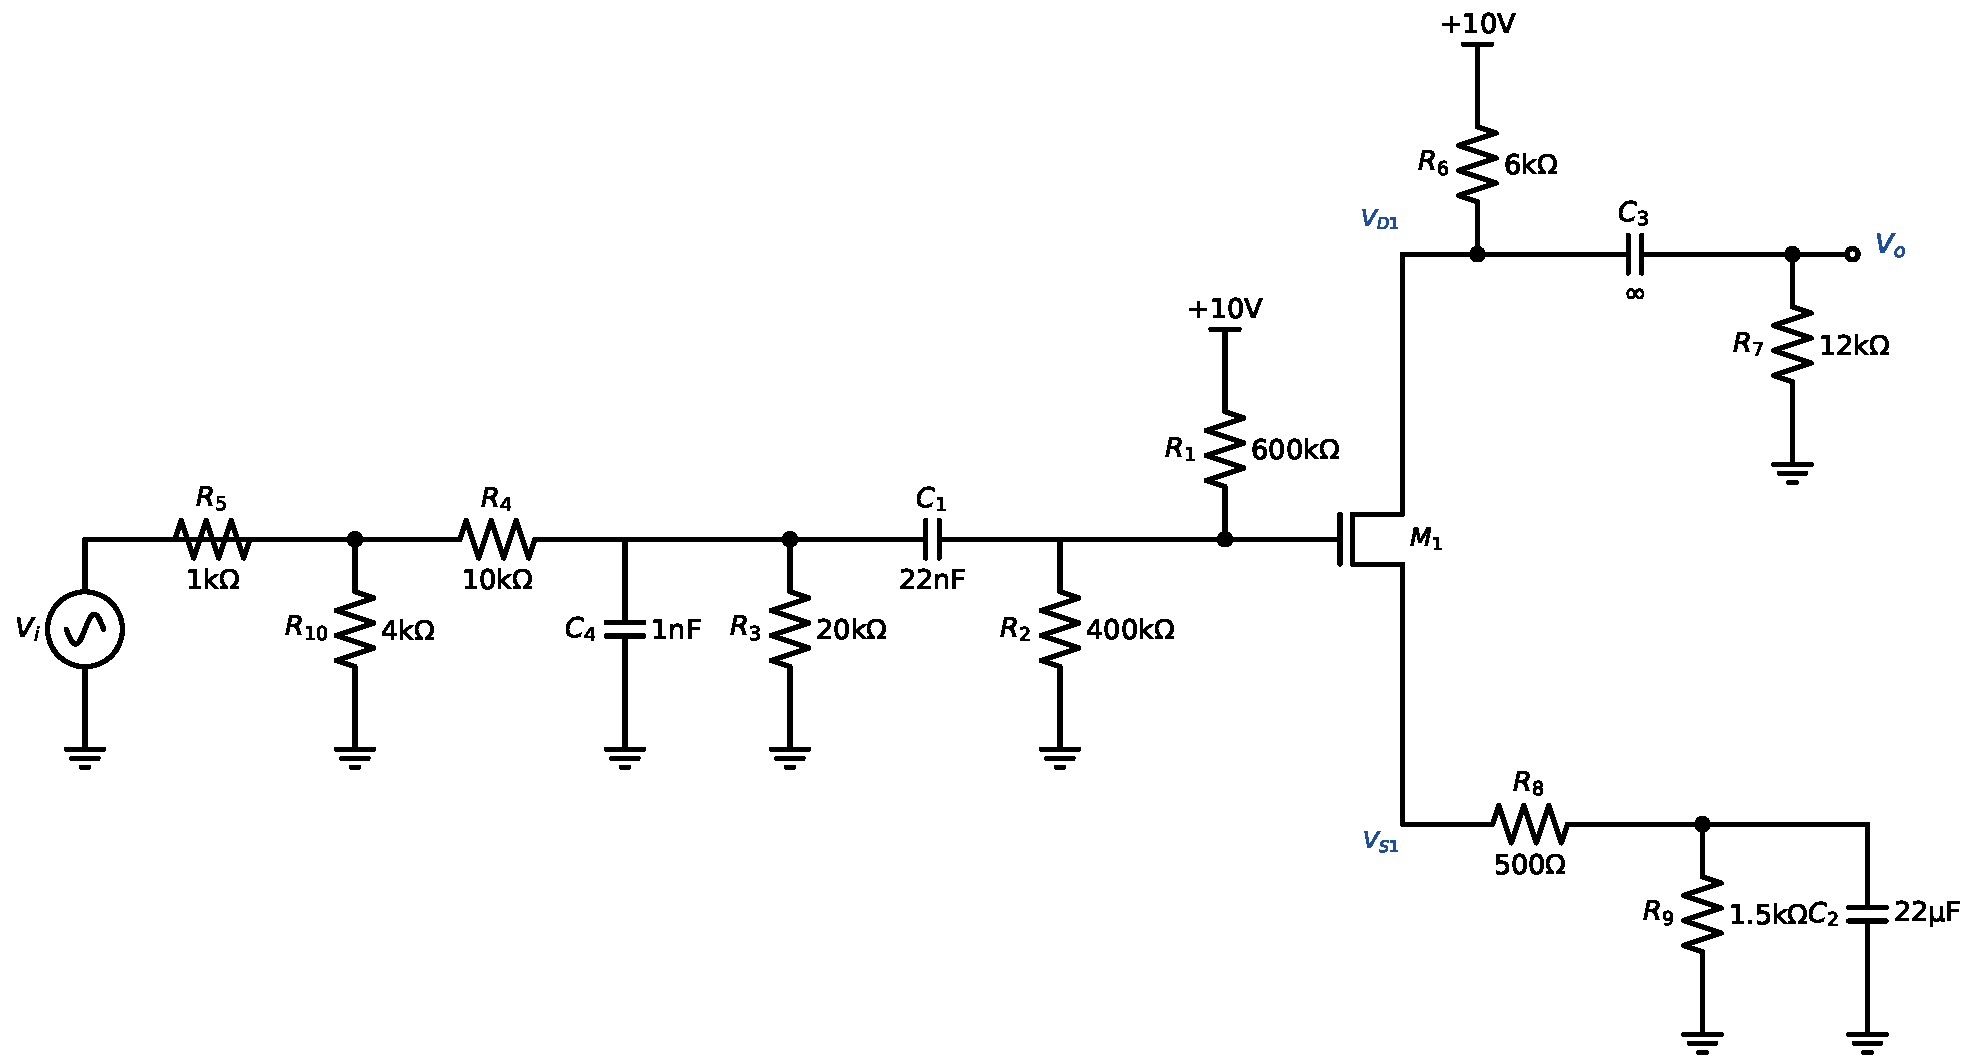
\includegraphics[width=0.9\linewidth,height=6cm,keepaspectratio]{p16_circuit}\end{center}
\solstep{1}{DC currents and transconductances}The DC drain currents are given: $I_{D1} = 726\,\mu \mathrm{A}$. For AC every supply is ground and every ``$\infty$'' capacitor is a short. Transconductances (tool T4):\begin{align*}
g_{m1} &= k_{1}V_{ov1} = \sqrt{2k_{1}I_{D1}} = \sqrt{2\cdot1.1\,\mathrm{m}\mathrm{A/V^2}\cdot726\,\mu \mathrm{A}} = 1.26\,\mathrm{m}\mathrm{A/V},\qquad \frac{1}{g_{m1}} = 791\,\Omega\quad(V_{ov1} = 1.15\,\mathrm{V})
\end{align*}

\solstep{2}{Thevenin equivalent of the input network}Between $v_i$ and the gate of $M_{1}$ there is a whole network (with KCL: one equation per node, in $s$). The transistor touches it only at its gate, so replace it by its Thevenin pair $(V_{th}(s), Z_{th}(s))$ seen from there (tool T5), marching from the far end: At $V_{x2}$ combine in parallel $R_{5}$ to $v_i$, $R_{10}$ to $0$ (Millman): \[V_{th} = \frac{\sum V_k/Z_k}{\sum 1/Z_k} = 0.8\,v_i,\qquad Z_{th} = 1\,\mathrm{k}\Omega \| 4\,\mathrm{k}\Omega = 800\,\Omega\] Through $R_{4}$ in series: $Z_{th}$ grows by $R_{4}$: $(V_{th}, Z_{th}) = (0.8\,v_i,\ 10.8\,\mathrm{k}\Omega)$. At $V_{x1}$ combine in parallel the part already reduced, $R_{3}$ to $0$, $C_{4}$ to $0$ (Millman): \[V_{th} = \frac{\sum V_k/Z_k}{\sum 1/Z_k} = \dfrac{74100}{s + 1.43\times 10^{5}}\,v_i,\qquad Z_{th} = 10.8\,\mathrm{k}\Omega \| 20\,\mathrm{k}\Omega \| \dfrac{10^{9}}{s} = \dfrac{10^{9}}{s + 1.43\times 10^{5}}\] Through $C_{1}$ in series: $Z_{th}$ grows by $\frac{1}{sC_{1}}$: $(V_{th}, Z_{th}) = (\dfrac{74100}{s + 1.43\times 10^{5}}\,v_i,\ \dfrac{1.05\times 10^{9}\,s + 6.48\times 10^{12}}{s^{2} + 1.43\times 10^{5}\,s})$. At $V_{G1}$ combine in parallel the part already reduced, $R_{1}$ to $0$, $R_{2}$ to $0$ (Millman): \[V_{th} = \frac{\sum V_k/Z_k}{\sum 1/Z_k} = \dfrac{74100\,s}{s^{2} + 1.47\times 10^{5}\,s + 2.7\times 10^{7}}\,v_i,\qquad Z_{th} = \dfrac{1.05\times 10^{9}\,s + 6.48\times 10^{12}}{s^{2} + 1.43\times 10^{5}\,s} \| 600\,\mathrm{k}\Omega \| 400\,\mathrm{k}\Omega = \dfrac{1.05\times 10^{9}\,s + 6.48\times 10^{12}}{s^{2} + 1.47\times 10^{5}\,s + 2.7\times 10^{7}}\] No current flows into the gate, so $Z_{th}$ plays no role: \[\frac{v_{g1}}{v_i} = \frac{V_{th}}{v_i} = \dfrac{74100\,s}{s^{2} + 1.47\times 10^{5}\,s + 2.7\times 10^{7}}\]
\solstep{3}{Rest of the signal path}Input resistance of every stage, from the last back to the first (each one loads the stage before it):\begin{align*}
R_{i1} &= Z_{gate,1} = \infty\quad\text{(input at the gate: it loads nothing)}
\end{align*}
Multiply the node-to-node gains along the signal path (tool T4):\[
H(s) = \frac{v_{d1}}{v_{g1}}
\]
\begin{align*}
\frac{v_{d1}}{v_{g1}} &= -\frac{Z_{D1}}{1/g_{m1} + Z_{S1}},\quad Z_{D1} = R_{6} \parallel R_{7},\ Z_{S1} = R_{8} + \left(R_{9} \parallel \frac{1}{sC_{2}}\right)\ \Rightarrow\ \dfrac{-3.1\,s - 93.9}{s + 65.5}
\end{align*}

\solstep{4}{Transfer function}Multiply and simplify:\[
H(s) = \dfrac{-2.29\times 10^{5}\,s^{2} - 6.95\times 10^{6}\,s}{s^{3} + 1.47\times 10^{5}\,s^{2} + 3.66\times 10^{7}\,s + 1.77\times 10^{9}}
\]

\solstep{5}{Standard (Bode-ready) form}Find the roots. Every root $s=-p$ of the denominator is a \emph{pole}, every root $s=-z$ of the numerator is a \emph{zero}; $|p|$ and $|z|$ are the corner frequencies (rad/s).
\begin{itemize}[leftmargin=*,itemsep=2pt]
\item Numerator: it has the factor $s$ $\Rightarrow$ 1 zero at $s=0$.
\item Numerator (after taking out the $s$ factor): $-2.29\times 10^{5}\,s - 6.95\times 10^{6}$; divide by the leading coefficient $-2.29\times 10^{5}$ (this does not move the roots): $s + 30.3$; $s + 30.3 = 0 \Rightarrow s = -30.3$.
\item Denominator: $s^{3} + 1.47\times 10^{5}\,s^{2} + 3.66\times 10^{7}\,s + 1.77\times 10^{9}$; this is degree 3: use a calculator's polynomial solver (or \texttt{numpy.roots}) $\Rightarrow s = -65.5,\ -184,\ -1.47\times 10^{5}$.
\end{itemize}

Factored form (leading coefficient in front):
\[
H(s) = -2.29\times 10^{5}\,\dfrac{s(s+30.3)}{(s+65.5)(s+184)(s+1.47\times 10^{5})}
\]

Bode-ready form: rewrite every $(s+p) = p\left(1+\frac{s}{p}\right)$ and $(s+z) = z\left(1+\frac{s}{z}\right)$, and collect all constants into $K$. Each $s$ in the numerator is paired with one of the \emph{lowest} poles as $\frac{s}{s+p}$ (that factor is $\approx 1$ above $p$). Then every factor except $K$ is $\approx 1$ inside the pass-band:
\[
H(s) = -0.257\,\dfrac{s}{s+2\pi\cdot 10.4}\,\left(1+\dfrac{s}{2\pi\cdot 4.82}\right)\,\dfrac{1}{1+\dfrac{s}{2\pi\cdot 29.3}}\,\dfrac{1}{1+\dfrac{s}{2\pi\cdot 23.4\mathrm{k}}},\qquad K = -0.257
\]

\begin{center}\renewcommand{\arraystretch}{1.35}
\begin{tabular}{cccc}
\toprule
type & $\omega_c$ (rad/s) & $f_c=\omega_c/2\pi$ & slope change \\
\midrule
zero & $30.3$ & 4.82 Hz & $+20$ dB/dec \\
pole & $65.5$ & 10.4 Hz & $-20$ dB/dec \\
pole & $184$ & 29.3 Hz & $-20$ dB/dec \\
pole & $1.47\times 10^{5}$ & 23.4 kHz & $-20$ dB/dec \\
\bottomrule
\end{tabular}\end{center}

\solstep{6}{Magnitude Bode plot}Below every corner $|H(s)|\approx 0.00393\,s$, so the plot starts with a slope of $+20$\,dB/dec. Then, moving right, each pole bends the line down by 20\,dB/dec and each zero bends it up by 20\,dB/dec (tool T6):
\begin{center}\renewcommand{\arraystretch}{1.35}
\begin{tabular}{lcl}
\toprule
frequency range & slope & asymptote level \\
\midrule
$f<$ 4.82 Hz & $+20$ dB/dec & -18.5 dB at end \\
4.82 Hz -- 10.4 Hz & $+40$ dB/dec & -18.5 dB at start, -5.09 dB at end \\
10.4 Hz -- 29.3 Hz & $+20$ dB/dec & -5.09 dB at start, 3.88 dB at end \\
29.3 Hz -- 23.4 kHz & $0$ dB/dec (flat) & 3.88 dB at start, 3.88 dB at end \\
$f>$ 23.4 kHz & $-20$ dB/dec & 3.88 dB at start \\
\bottomrule
\end{tabular}\end{center}

\begin{center}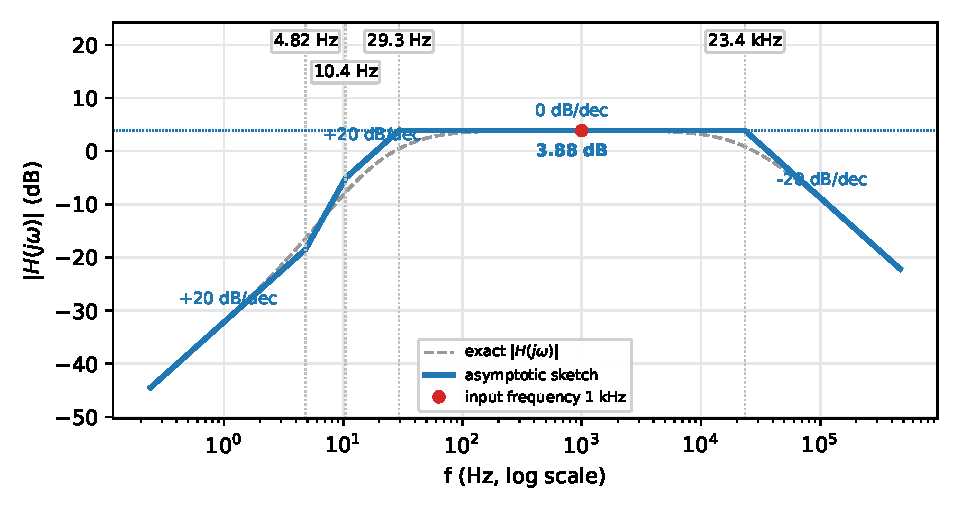
\includegraphics[width=0.78\linewidth,height=6.5cm,keepaspectratio]{p16_bode}\end{center}

{\small Blue: the straight-line sketch you are expected to draw. Dashed grey: the exact curve (about 3\,dB below the corner of an isolated pole). Red dot: the input frequency of Step 7.}
\solstep{7}{Steady-state output}The input is $V_i(t) = 0.01\sin\left(2\pi\cdot 1000\,t\right)$, so $\omega_{in} = 2\pi\cdot 1000 = 6280$\,rad/s. Put $s=j\omega_{in}$ in each factor (tool T5): magnitudes multiply, angles add.
{\small Rules: $\left|\frac{s}{s+p}\right| = \frac{\omega}{\sqrt{\omega^2+p^2}}$, $\angle = \frac{\pi}{2}-\tan^{-1}\frac{\omega}{p}$;\quad $\left|\frac{1}{1+s/p}\right| = \frac{1}{\sqrt{1+(\omega/p)^2}}$, $\angle = -\tan^{-1}\frac{\omega}{p}$;\quad $\left|1+\frac{s}{z}\right| = \sqrt{1+(\omega/z)^2}$, $\angle = \tan^{-1}\frac{\omega}{z}$;\quad a negative $K$ adds $-\pi$.}
\begin{center}\renewcommand{\arraystretch}{1.35}
\begin{tabular}{ccc}
\toprule
factor & magnitude & angle (rad) \\
\midrule
$-0.257$ & $0.2574$ & $-3.14$ \\
$\rule[-1.1em]{0pt}{2.8em}\dfrac{s}{s+2\pi\cdot 10.4}$ & $0.9999$ & $0.0104$ \\
$\rule[-1.1em]{0pt}{2.8em}\left(1+\dfrac{s}{2\pi\cdot 4.82}\right)$ & $207.3$ & $1.57$ \\
$\rule[-1.7em]{0pt}{4em}\dfrac{1}{1+\dfrac{s}{2\pi\cdot 29.3}}$ & $0.02927$ & $-1.54$ \\
$\rule[-1.7em]{0pt}{4em}\dfrac{1}{1+\dfrac{s}{2\pi\cdot 23.4\mathrm{k}}}$ & $0.9991$ & $-0.0428$ \\
\textbf{total} & $\mathbf{1.561}$ (product) & $\mathbf{-3.15}$ (sum) \\
\bottomrule
\end{tabular}\end{center}

\begin{align*}
|H(j\omega_{in})| &= 1.56, \qquad \angle H(j\omega_{in}) = -3.15\ \mathrm{rad} \\
v_{o,ac}(t) &= 1.56\times 0.01\,\sin\left(2\pi\cdot 1000\,t - 3.15\right) = 0.0156\,\sin\left(2\pi\cdot 1000\,t - 3.15\right)
\end{align*}

\[
\boxed{V_o(t) = 0.0156\,\sin\left(2\pi\cdot 1000\,t - 3.15\right)\ \mathrm{V}}
\]

\begin{ansbox}
$H(s) = -0.257\,\dfrac{s}{s+2\pi\cdot 10.4}\,\left(1+\dfrac{s}{2\pi\cdot 4.82}\right)\,\dfrac{1}{1+\dfrac{s}{2\pi\cdot 29.3}}\,\dfrac{1}{1+\dfrac{s}{2\pi\cdot 23.4\mathrm{k}}}$\quad (corners: 4.82 Hz, 10.4 Hz, 29.3 Hz, 23.4 kHz)\\[4pt]
$V_o(t) = 0.0156\,\sin\left(2\pi\cdot 1000\,t - 3.15\right)\ \mathrm{V}$
\end{ansbox}

\newpage
\subsection*{Solution 5F.17 \hfill Hard}
\begin{center}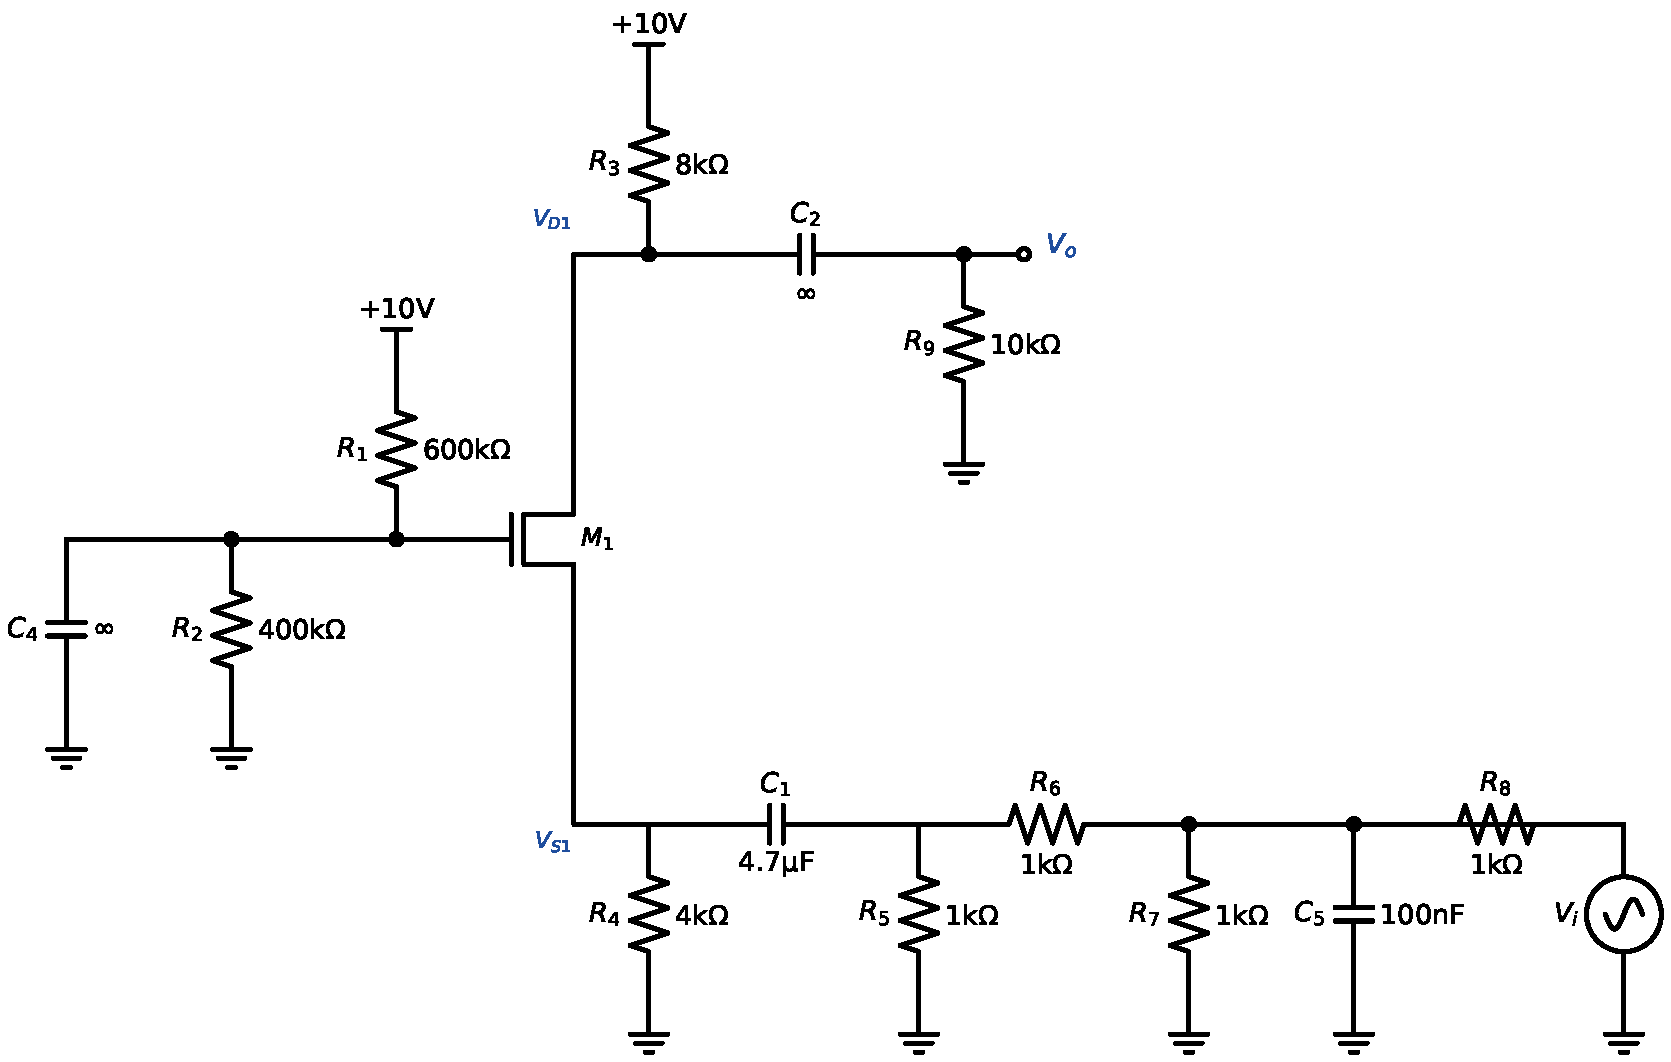
\includegraphics[width=0.9\linewidth,height=6cm,keepaspectratio]{p17_circuit}\end{center}
\solstep{1}{DC currents and transconductances}The DC drain currents are given: $I_{D1} = 429\,\mu \mathrm{A}$. For AC every supply is ground and every ``$\infty$'' capacitor is a short. Transconductances (tool T4):\begin{align*}
g_{m1} &= k_{1}V_{ov1} = \sqrt{2k_{1}I_{D1}} = \sqrt{2\cdot1.1\,\mathrm{m}\mathrm{A/V^2}\cdot429\,\mu \mathrm{A}} = 972\,\mu \mathrm{A/V},\qquad \frac{1}{g_{m1}} = 1.03\,\mathrm{k}\Omega\quad(V_{ov1} = 0.883\,\mathrm{V})
\end{align*}

\solstep{2}{Thevenin equivalent of the input network}Between $v_i$ and the source of $M_{1}$ there is a whole network (with KCL: one equation per node, in $s$). The transistor touches it only at its source, so replace it by its Thevenin pair $(V_{th}(s), Z_{th}(s))$ seen from there (tool T5), marching from the far end: At $V_{x2}$ combine in parallel $R_{7}$ to $0$, $C_{5}$ to $0$, $R_{8}$ to $v_i$ (Millman): \[V_{th} = \frac{\sum V_k/Z_k}{\sum 1/Z_k} = \dfrac{10000}{s + 20000}\,v_i,\qquad Z_{th} = 1\,\mathrm{k}\Omega \| \dfrac{10^{7}}{s} \| 1\,\mathrm{k}\Omega = \dfrac{10^{7}}{s + 20000}\] Through $R_{6}$ in series: $Z_{th}$ grows by $R_{6}$: $(V_{th}, Z_{th}) = (\dfrac{10000}{s + 20000}\,v_i,\ \dfrac{1000\,s + 3\times 10^{7}}{s + 20000})$. At $V_{x1}$ combine in parallel the part already reduced, $R_{5}$ to $0$ (Millman): \[V_{th} = \frac{\sum V_k/Z_k}{\sum 1/Z_k} = \dfrac{5000}{s + 25000}\,v_i,\qquad Z_{th} = \dfrac{1000\,s + 3\times 10^{7}}{s + 20000} \| 1\,\mathrm{k}\Omega = \dfrac{500\,s + 1.5\times 10^{7}}{s + 25000}\] Through $C_{1}$ in series: $Z_{th}$ grows by $\frac{1}{sC_{1}}$: $(V_{th}, Z_{th}) = (\dfrac{5000}{s + 25000}\,v_i,\ \dfrac{500\,s^{2} + 1.52\times 10^{7}\,s + 5.32\times 10^{9}}{s^{2} + 25000\,s})$. At $V_{S1}$ combine in parallel the part already reduced, $R_{4}$ to $0$ (Millman): \[V_{th} = \frac{\sum V_k/Z_k}{\sum 1/Z_k} = \dfrac{4440\,s}{s^{2} + 25600\,s + 1.18\times 10^{6}}\,v_i,\qquad Z_{th} = \dfrac{500\,s^{2} + 1.52\times 10^{7}\,s + 5.32\times 10^{9}}{s^{2} + 25000\,s} \| 4\,\mathrm{k}\Omega = \dfrac{444\,s^{2} + 1.35\times 10^{7}\,s + 4.73\times 10^{9}}{s^{2} + 25600\,s + 1.18\times 10^{6}}\] The source of the common-gate stage presents $1/g_{m1} = 1.03\,\mathrm{k}\Omega$ to this Thevenin source, a voltage divider: \[\frac{v_{s1}}{v_i} = \frac{V_{th}}{v_i}\cdot\frac{1/g_{m1}}{Z_{th} + 1/g_{m1}} = \dfrac{3100\,s}{s^{2} + 27100\,s + 4.03\times 10^{6}}\]
\solstep{3}{Rest of the signal path}Input resistance of every stage, from the last back to the first (each one loads the stage before it):\begin{align*}
R_{i1} &= Z_{source,1} = \frac{1}{g_{m1}} = 1.03\,\mathrm{k}\Omega\quad\text{(common gate)}
\end{align*}
Multiply the node-to-node gains along the signal path (tool T4):\[
H(s) = \frac{v_{d1}}{v_{s1}}
\]
\begin{align*}
\frac{v_{d1}}{v_{s1}} &= \frac{Z_{D1}}{1/g_{m1}},\quad Z_{D1} = R_{3} \parallel R_{9}\ \Rightarrow\ 4.32
\end{align*}

\solstep{4}{Transfer function}Multiply and simplify:\[
H(s) = \dfrac{13400\,s}{s^{2} + 27100\,s + 4.03\times 10^{6}}
\]

\solstep{5}{Standard (Bode-ready) form}Find the roots. Every root $s=-p$ of the denominator is a \emph{pole}, every root $s=-z$ of the numerator is a \emph{zero}; $|p|$ and $|z|$ are the corner frequencies (rad/s).
\begin{itemize}[leftmargin=*,itemsep=2pt]
\item Numerator: it has the factor $s$ $\Rightarrow$ 1 zero at $s=0$.
\item Denominator: $s^{2} + 27100\,s + 4.03\times 10^{6}$; quadratic formula:\[
s = \frac{-27100 \pm \sqrt{(27100)^2 - 4(4.03\times 10^{6})}}{2} = \frac{-27100 \pm 26800}{2} \Rightarrow s = -150,\ -26900
\]

\end{itemize}

Factored form (leading coefficient in front):
\[
H(s) = 13400\,\dfrac{s}{(s+150)(s+26900)}
\]

Bode-ready form: rewrite every $(s+p) = p\left(1+\frac{s}{p}\right)$ and $(s+z) = z\left(1+\frac{s}{z}\right)$, and collect all constants into $K$. Each $s$ in the numerator is paired with one of the \emph{lowest} poles as $\frac{s}{s+p}$ (that factor is $\approx 1$ above $p$). Then every factor except $K$ is $\approx 1$ inside the pass-band:
\[
H(s) = 0.498\,\dfrac{s}{s+2\pi\cdot 23.9}\,\dfrac{1}{1+\dfrac{s}{2\pi\cdot 4.28\mathrm{k}}},\qquad K = 0.498
\]

\begin{center}\renewcommand{\arraystretch}{1.35}
\begin{tabular}{cccc}
\toprule
type & $\omega_c$ (rad/s) & $f_c=\omega_c/2\pi$ & slope change \\
\midrule
pole & $150$ & 23.9 Hz & $-20$ dB/dec \\
pole & $26900$ & 4.28 kHz & $-20$ dB/dec \\
\bottomrule
\end{tabular}\end{center}

\solstep{6}{Magnitude Bode plot}Below every corner $|H(s)|\approx 0.00332\,s$, so the plot starts with a slope of $+20$\,dB/dec. Then, moving right, each pole bends the line down by 20\,dB/dec and each zero bends it up by 20\,dB/dec (tool T6):
\begin{center}\renewcommand{\arraystretch}{1.35}
\begin{tabular}{lcl}
\toprule
frequency range & slope & asymptote level \\
\midrule
$f<$ 23.9 Hz & $+20$ dB/dec & -6.05 dB at end \\
23.9 Hz -- 4.28 kHz & $0$ dB/dec (flat) & -6.05 dB at start, -6.05 dB at end \\
$f>$ 4.28 kHz & $-20$ dB/dec & -6.05 dB at start \\
\bottomrule
\end{tabular}\end{center}

The flat (pass-band) level is $20\log_{10}|K| = 20\log_{10}0.498 = -6.05$\,dB.
\begin{center}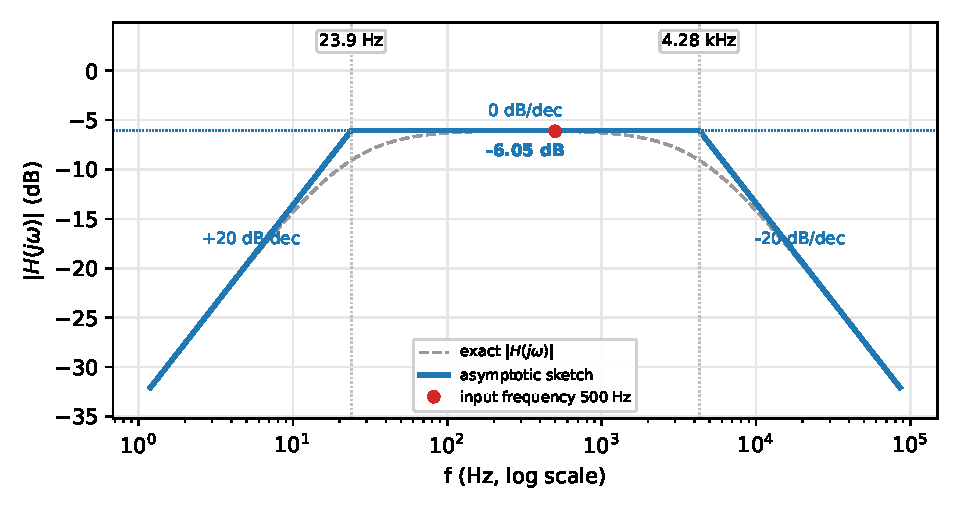
\includegraphics[width=0.78\linewidth,height=6.5cm,keepaspectratio]{p17_bode}\end{center}

{\small Blue: the straight-line sketch you are expected to draw. Dashed grey: the exact curve (about 3\,dB below the corner of an isolated pole). Red dot: the input frequency of Step 7.}
\solstep{7}{Steady-state output}The input is $V_i(t) = 0.01\sin\left(2\pi\cdot 500\,t\right)$, so $\omega_{in} = 2\pi\cdot 500 = 3140$\,rad/s. Put $s=j\omega_{in}$ in each factor (tool T5): magnitudes multiply, angles add.
{\small Rules: $\left|\frac{s}{s+p}\right| = \frac{\omega}{\sqrt{\omega^2+p^2}}$, $\angle = \frac{\pi}{2}-\tan^{-1}\frac{\omega}{p}$;\quad $\left|\frac{1}{1+s/p}\right| = \frac{1}{\sqrt{1+(\omega/p)^2}}$, $\angle = -\tan^{-1}\frac{\omega}{p}$;\quad $\left|1+\frac{s}{z}\right| = \sqrt{1+(\omega/z)^2}$, $\angle = \tan^{-1}\frac{\omega}{z}$;\quad a negative $K$ adds $-\pi$.}
\begin{center}\renewcommand{\arraystretch}{1.35}
\begin{tabular}{ccc}
\toprule
factor & magnitude & angle (rad) \\
\midrule
$0.498$ & $0.4982$ & $0$ \\
$\rule[-1.1em]{0pt}{2.8em}\dfrac{s}{s+2\pi\cdot 23.9}$ & $0.9989$ & $0.0477$ \\
$\rule[-1.7em]{0pt}{4em}\dfrac{1}{1+\dfrac{s}{2\pi\cdot 4.28\mathrm{k}}}$ & $0.9933$ & $-0.116$ \\
\textbf{total} & $\mathbf{0.4943}$ (product) & $\mathbf{-0.0685}$ (sum) \\
\bottomrule
\end{tabular}\end{center}

\begin{align*}
|H(j\omega_{in})| &= 0.494, \qquad \angle H(j\omega_{in}) = -0.0685\ \mathrm{rad} \\
v_{o,ac}(t) &= 0.494\times 0.01\,\sin\left(2\pi\cdot 500\,t - 0.0685\right) = 0.00494\,\sin\left(2\pi\cdot 500\,t - 0.0685\right)
\end{align*}

\[
\boxed{V_o(t) = 0.00494\,\sin\left(2\pi\cdot 500\,t - 0.0685\right)\ \mathrm{V}}
\]

\begin{ansbox}
$H(s) = 0.498\,\dfrac{s}{s+2\pi\cdot 23.9}\,\dfrac{1}{1+\dfrac{s}{2\pi\cdot 4.28\mathrm{k}}}$\quad (corners: 23.9 Hz, 4.28 kHz)\\[4pt]
$V_o(t) = 0.00494\,\sin\left(2\pi\cdot 500\,t - 0.0685\right)\ \mathrm{V}$
\end{ansbox}

\newpage
\subsection*{Solution 5F.18 \hfill Hard}
\begin{center}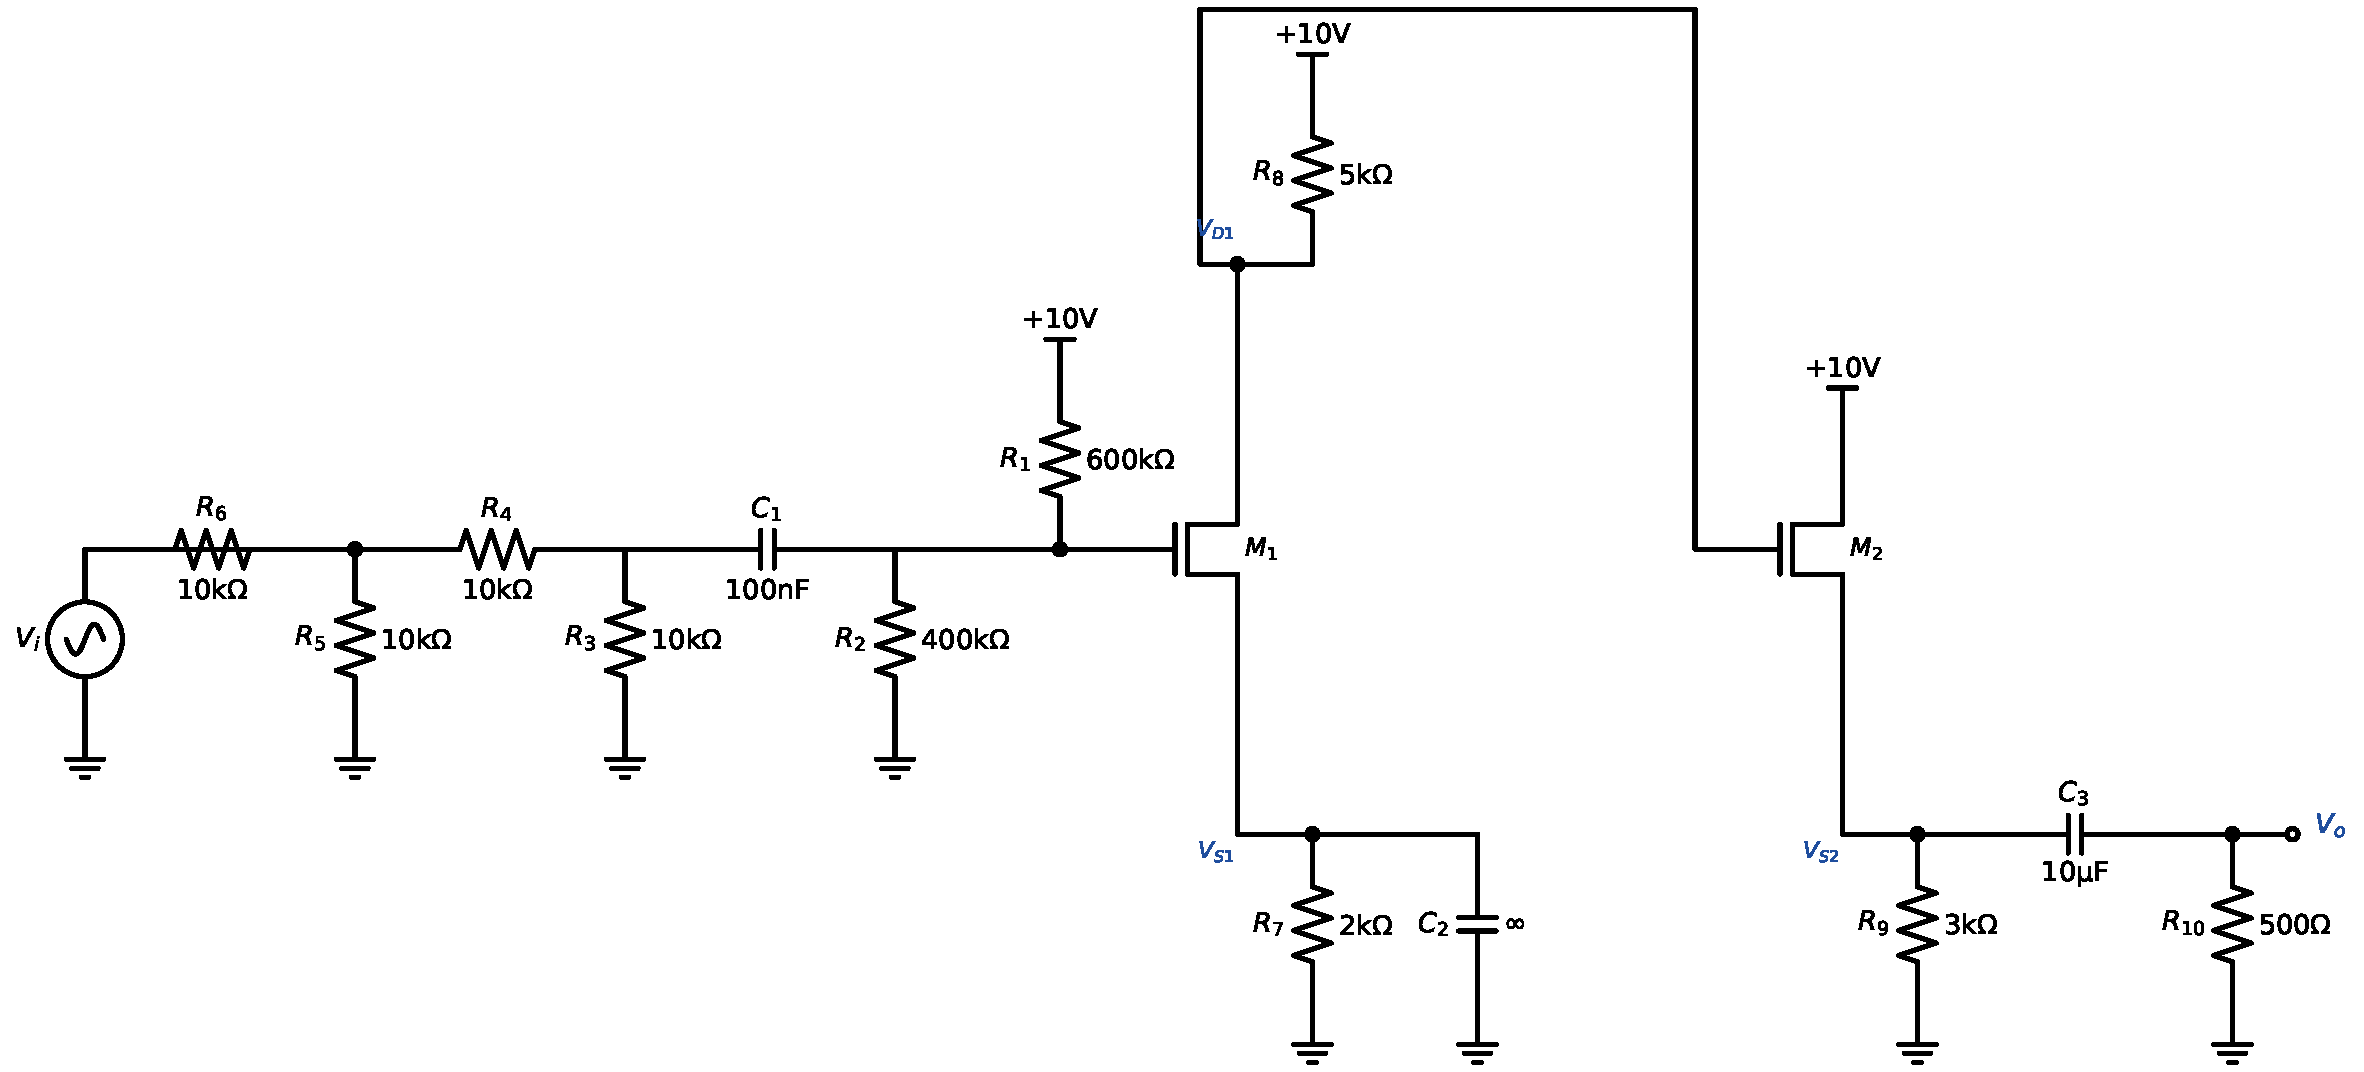
\includegraphics[width=0.9\linewidth,height=6cm,keepaspectratio]{p18_circuit}\end{center}
\solstep{1}{DC currents and transconductances}The DC drain currents are given: $I_{D1} = 726\,\mu \mathrm{A}$, $I_{D2} = 1.17\,\mathrm{m}\mathrm{A}$. For AC every supply is ground and every ``$\infty$'' capacitor is a short. Transconductances (tool T4):\begin{align*}
g_{m1} &= k_{1}V_{ov1} = \sqrt{2k_{1}I_{D1}} = \sqrt{2\cdot1.1\,\mathrm{m}\mathrm{A/V^2}\cdot726\,\mu \mathrm{A}} = 1.26\,\mathrm{m}\mathrm{A/V},\qquad \frac{1}{g_{m1}} = 791\,\Omega\quad(V_{ov1} = 1.15\,\mathrm{V}) \\
g_{m2} &= k_{2}V_{ov2} = \sqrt{2k_{2}I_{D2}} = \sqrt{2\cdot1.1\,\mathrm{m}\mathrm{A/V^2}\cdot1.17\,\mathrm{m}\mathrm{A}} = 1.6\,\mathrm{m}\mathrm{A/V},\qquad \frac{1}{g_{m2}} = 623\,\Omega\quad(V_{ov2} = 1.46\,\mathrm{V})
\end{align*}

\solstep{2}{Thevenin equivalent of the input network}Between $v_i$ and the gate of $M_{1}$ there is a whole network (with KCL: one equation per node, in $s$). The transistor touches it only at its gate, so replace it by its Thevenin pair $(V_{th}(s), Z_{th}(s))$ seen from there (tool T5), marching from the far end: At $V_{x2}$ combine in parallel $R_{5}$ to $0$, $R_{6}$ to $v_i$ (Millman): \[V_{th} = \frac{\sum V_k/Z_k}{\sum 1/Z_k} = 0.5\,v_i,\qquad Z_{th} = 10\,\mathrm{k}\Omega \| 10\,\mathrm{k}\Omega = 5\,\mathrm{k}\Omega\] Through $R_{4}$ in series: $Z_{th}$ grows by $R_{4}$: $(V_{th}, Z_{th}) = (0.5\,v_i,\ 15\,\mathrm{k}\Omega)$. At $V_{x1}$ combine in parallel the part already reduced, $R_{3}$ to $0$ (Millman): \[V_{th} = \frac{\sum V_k/Z_k}{\sum 1/Z_k} = 0.2\,v_i,\qquad Z_{th} = 15\,\mathrm{k}\Omega \| 10\,\mathrm{k}\Omega = 6\,\mathrm{k}\Omega\] Through $C_{1}$ in series: $Z_{th}$ grows by $\frac{1}{sC_{1}}$: $(V_{th}, Z_{th}) = (0.2\,v_i,\ \dfrac{6000\,s + 10^{7}}{s})$. At $V_{G1}$ combine in parallel the part already reduced, $R_{1}$ to $0$, $R_{2}$ to $0$ (Millman): \[V_{th} = \frac{\sum V_k/Z_k}{\sum 1/Z_k} = \dfrac{0.195\,s}{s + 40.7}\,v_i,\qquad Z_{th} = \dfrac{6000\,s + 10^{7}}{s} \| 600\,\mathrm{k}\Omega \| 400\,\mathrm{k}\Omega = \dfrac{5850\,s + 9.76\times 10^{6}}{s + 40.7}\] No current flows into the gate, so $Z_{th}$ plays no role: \[\frac{v_{g1}}{v_i} = \frac{V_{th}}{v_i} = \dfrac{0.195\,s}{s + 40.7}\]
\solstep{3}{Rest of the signal path}Input resistance of every stage, from the last back to the first (each one loads the stage before it):\begin{align*}
R_{i1} &= Z_{gate,1} = \infty\quad\text{(input at the gate: it loads nothing)} \\
R_{i2} &= Z_{gate,2} = \infty\quad\text{(input at the gate: it loads nothing)}
\end{align*}
Multiply the node-to-node gains along the signal path (tool T4):\[
H(s) = \frac{v_{d1}}{v_{g1}}\cdot\frac{v_{s2}}{v_{g2}}\cdot\frac{v_o}{v_{s2}}
\]
\begin{align*}
\frac{v_{d1}}{v_{g1}} &= -\frac{Z_{D1}}{1/g_{m1} + Z_{S1}},\quad Z_{D1} = R_{8},\ Z_{S1} = 0\ \Rightarrow\ -6.32 \\
\frac{v_{s2}}{v_{g2}} &= \frac{Z_{S2}}{1/g_{m2} + Z_{S2}},\quad Z_{S2} = R_{9} \parallel \left(\frac{1}{sC_{3}} + R_{10}\right)\ \Rightarrow\ \dfrac{0.408\,s + 81.5}{s + 98.4} \\
\frac{v_o}{v_{s2}} &= \frac{R_{10}}{\frac{1}{sC_{3}} + R_{10}} = \dfrac{s}{s + 200}
\end{align*}

\solstep{4}{Transfer function}Multiply and simplify:\[
H(s) = \dfrac{-0.502\,s^{2}}{s^{2} + 139\,s + 4000}
\]

\solstep{5}{Standard (Bode-ready) form}Find the roots. Every root $s=-p$ of the denominator is a \emph{pole}, every root $s=-z$ of the numerator is a \emph{zero}; $|p|$ and $|z|$ are the corner frequencies (rad/s).
\begin{itemize}[leftmargin=*,itemsep=2pt]
\item Numerator: it has the factor $s^2$ $\Rightarrow$ 2 zeros at $s=0$.
\item Denominator: $s^{2} + 139\,s + 4000$; quadratic formula:\[
s = \frac{-139 \pm \sqrt{(139)^2 - 4(4000)}}{2} = \frac{-139 \pm 57.8}{2} \Rightarrow s = -40.7,\ -98.4
\]

\end{itemize}

Factored form (leading coefficient in front):
\[
H(s) = -0.502\,\dfrac{s^{2}}{(s+40.7)(s+98.4)}
\]

Bode-ready form: rewrite every $(s+p) = p\left(1+\frac{s}{p}\right)$ and $(s+z) = z\left(1+\frac{s}{z}\right)$, and collect all constants into $K$. Each $s$ in the numerator is paired with one of the \emph{lowest} poles as $\frac{s}{s+p}$ (that factor is $\approx 1$ above $p$). Then every factor except $K$ is $\approx 1$ inside the pass-band:
\[
H(s) = -0.502\,\dfrac{s}{s+2\pi\cdot 6.47}\,\dfrac{s}{s+2\pi\cdot 15.7},\qquad K = -0.502
\]

\begin{center}\renewcommand{\arraystretch}{1.35}
\begin{tabular}{cccc}
\toprule
type & $\omega_c$ (rad/s) & $f_c=\omega_c/2\pi$ & slope change \\
\midrule
pole & $40.7$ & 6.47 Hz & $-20$ dB/dec \\
pole & $98.4$ & 15.7 Hz & $-20$ dB/dec \\
\bottomrule
\end{tabular}\end{center}

\solstep{6}{Magnitude Bode plot}Below every corner $|H(s)|\approx 1.26\times 10^{-4}\,s^2$, so the plot starts with a slope of $+40$\,dB/dec. Then, moving right, each pole bends the line down by 20\,dB/dec and each zero bends it up by 20\,dB/dec (tool T6):
\begin{center}\renewcommand{\arraystretch}{1.35}
\begin{tabular}{lcl}
\toprule
frequency range & slope & asymptote level \\
\midrule
$f<$ 6.47 Hz & $+40$ dB/dec & -13.7 dB at end \\
6.47 Hz -- 15.7 Hz & $+20$ dB/dec & -13.7 dB at start, -5.98 dB at end \\
$f>$ 15.7 Hz & $0$ dB/dec (flat) & -5.98 dB at start \\
\bottomrule
\end{tabular}\end{center}

The flat (pass-band) level is $20\log_{10}|K| = 20\log_{10}0.502 = -5.98$\,dB.
\begin{center}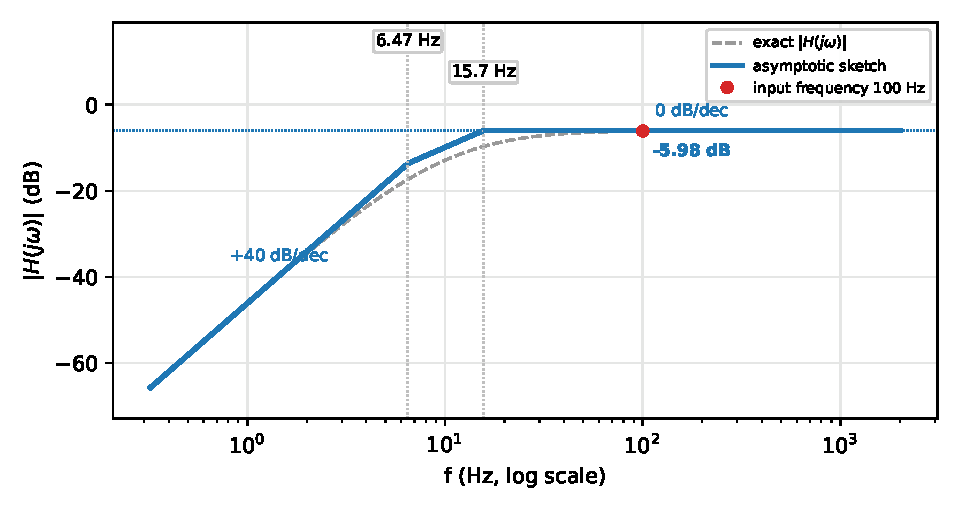
\includegraphics[width=0.78\linewidth,height=6.5cm,keepaspectratio]{p18_bode}\end{center}

{\small Blue: the straight-line sketch you are expected to draw. Dashed grey: the exact curve (about 3\,dB below the corner of an isolated pole). Red dot: the input frequency of Step 7.}
\solstep{7}{Steady-state output}The input is $V_i(t) = 0.01\sin\left(2\pi\cdot 100\,t\right)$, so $\omega_{in} = 2\pi\cdot 100 = 628$\,rad/s. Put $s=j\omega_{in}$ in each factor (tool T5): magnitudes multiply, angles add.
{\small Rules: $\left|\frac{s}{s+p}\right| = \frac{\omega}{\sqrt{\omega^2+p^2}}$, $\angle = \frac{\pi}{2}-\tan^{-1}\frac{\omega}{p}$;\quad $\left|\frac{1}{1+s/p}\right| = \frac{1}{\sqrt{1+(\omega/p)^2}}$, $\angle = -\tan^{-1}\frac{\omega}{p}$;\quad $\left|1+\frac{s}{z}\right| = \sqrt{1+(\omega/z)^2}$, $\angle = \tan^{-1}\frac{\omega}{z}$;\quad a negative $K$ adds $-\pi$.}
\begin{center}\renewcommand{\arraystretch}{1.35}
\begin{tabular}{ccc}
\toprule
factor & magnitude & angle (rad) \\
\midrule
$-0.502$ & $0.5024$ & $-3.14$ \\
$\rule[-1.1em]{0pt}{2.8em}\dfrac{s}{s+2\pi\cdot 6.47}$ & $0.9979$ & $0.0646$ \\
$\rule[-1.1em]{0pt}{2.8em}\dfrac{s}{s+2\pi\cdot 15.7}$ & $0.9879$ & $0.155$ \\
\textbf{total} & $\mathbf{0.4953}$ (product) & $\mathbf{-2.92}$ (sum) \\
\bottomrule
\end{tabular}\end{center}

\begin{align*}
|H(j\omega_{in})| &= 0.495, \qquad \angle H(j\omega_{in}) = -2.92\ \mathrm{rad} \\
v_{o,ac}(t) &= 0.495\times 0.01\,\sin\left(2\pi\cdot 100\,t - 2.92\right) = 0.00495\,\sin\left(2\pi\cdot 100\,t - 2.92\right)
\end{align*}

\[
\boxed{V_o(t) = 0.00495\,\sin\left(2\pi\cdot 100\,t - 2.92\right)\ \mathrm{V}}
\]

\begin{ansbox}
$H(s) = -0.502\,\dfrac{s}{s+2\pi\cdot 6.47}\,\dfrac{s}{s+2\pi\cdot 15.7}$\quad (corners: 6.47 Hz, 15.7 Hz)\\[4pt]
$V_o(t) = 0.00495\,\sin\left(2\pi\cdot 100\,t - 2.92\right)\ \mathrm{V}$
\end{ansbox}

\end{document}
